\documentclass[oneside,12pt,letterpaper]{book}
\setcounter{tocdepth}{3}
\setcounter{secnumdepth}{3}

%%%%%%%%%%%%%%%% for dev
% \includeonly{Chapter_1,Chapter_4}
%%%%%%%%%%%%%%%%
%%%%% CAMBIAR LA PRIMERA LINEA POR LA SIGUIENTE PARA LA MEMORIA DE PROYECTO %%%%%
%\documentclass[12pt,letterpaper,oneside]{book}

% Paquetes basicos ...
\usepackage[spanish, mexico]{babel}
\usepackage[utf8]{inputenc} % OJO!!!  => MANTENER ESTA LINEA PARA FACIL CONVERSION A WORD EN EL FUTURO ...
\usepackage{float,xcolor}
\usepackage{graphicx} 
\usepackage{array}
\usepackage{tabularx}
\usepackage{amssymb, amsmath}

% Paquetes extras ... 
\usepackage{subfigure}
% \usepackage{color}
\usepackage{anysize} 
\usepackage{breakcites}
\usepackage{enumitem}
\usepackage{blindtext}
\usepackage{hyperref}
% figuras
\usepackage{wrapfig}
\usepackage{lscape}
\usepackage{rotating}
\usepackage{epstopdf}

\usepackage{booktabs}
\usepackage{multirow}
% \usepackage[table,xcdraw]{xcolor}
\usepackage{listings} % para codigo fuente

% para los algoritmos
\usepackage{algorithm}
\usepackage{algorithmic}

\floatname{algorithm}{Algoritmo}
\renewcommand{\listalgorithmname}{Lista de algoritmos}
\renewcommand{\algorithmicrequire}{\textbf{Entrada:}}
\renewcommand{\algorithmicensure}{\textbf{Salida:}}
\renewcommand{\algorithmicend}{\textbf{fin}}
\renewcommand{\algorithmicif}{\textbf{Si}}
\renewcommand{\algorithmicthen}{\textbf{entonces:}}
\renewcommand{\algorithmicelse}{\textbf{Si no}}
\renewcommand{\algorithmicelsif}{\algorithmicelse,\ \algorithmicif}
\renewcommand{\algorithmicendif}{\algorithmicend\ \algorithmicif}
\renewcommand{\algorithmicfor}{\textbf{Para}}
\renewcommand{\algorithmicforall}{\textbf{Para todo}}
\renewcommand{\algorithmicdo}{\textbf{hacer:}}
\renewcommand{\algorithmicendfor}{\algorithmicend\ \algorithmicfor}
\renewcommand{\algorithmicwhile}{\textbf{Mientras}}
\renewcommand{\algorithmicendwhile}{\algorithmicend\ \algorithmicwhile}
\renewcommand{\algorithmicloop}{\textbf{repetir:}}
\renewcommand{\algorithmicendloop}{\algorithmicend\ \algorithmicloop}
\renewcommand{\algorithmicrepeat}{\textbf{repetir:}}
\renewcommand{\algorithmicuntil}{\textbf{hasta que:}}
\renewcommand{\algorithmicprint}{\textbf{Imprimir}} 
\renewcommand{\algorithmicreturn}{\textbf{Retornar:}} 
\renewcommand{\algorithmictrue}{\textbf{verdadero }} 
\renewcommand{\algorithmicfalse}{\textbf{falso }} 
 % mi archivo de traducción

\usepackage{lipsum}
\usepackage{courier}

\usepackage{tikz}
\def\checkmark{\tikz\fill[scale=0.4](0,.35) -- (.25,0) -- (1,.7) -- (.25,.15) -- cycle;}

\lstset{basicstyle=\footnotesize\ttfamily, breaklines=true}
% %% para que aparezca Capitulo
% \usepackage{tocloft}

% \renewcommand{\cftchappresnum}{Capítulo }
% \renewcommand{\cftchapaftersnum}{:}
% \renewcommand{\cftchapnumwidth}{25mm}


\begin{document}
\marginsize{2.5cm}{2cm}{2cm}{2cm} 

% Para que no aparezca la numeracion en el pie de pagina de todo el documento ...
%\pagestyle{empty}


%%%%%% ******  INICIO CARATULA ***** %%%%%%%%%
% Especificaciones de la caratula PPG

\begin{titlepage}
    \begin{center}
    \vspace*{-0.5in}
    \begin{large}
    \textbf{UNIVERSIDAD MAYOR DE SAN ANDRÉS}\\
    \vspace*{0.15in}
    \textbf{FACULTAD DE INGENIERÍA}\\
    \vspace*{0.15in}
    \textbf{CARRERA DE INGENIERÍA ELECTRÓNICA}\\
    \vspace*{0.1in}
    \end{large}
    % Logo UMSA
    \begin{figure}[htb]
    \begin{center}
    
\includegraphics[width=8cm]{img/umsa.jpg}
    % 
\includegraphics{img/umsa.jpg}
    \end{center}
    \end{figure}
    \begin{Large}
    \textbf{PROYECTO DE GRADO} 
    \end{Large}
    \vspace*{0.4in}
    
    \begin{normalsize}
    \textbf{``Aprendizaje fin a fin para la conducción autónoma de vehículos domésticos usando visión artificial y redes neuronales convolucionales''} \\
    \end{normalsize}
    
    \vspace*{0.2in}
    
    \begin{large}
    \textbf{POSTULANTE:} JOSE EDUARDO LARUTA ESPEJO\\
    \end{large}
    
    \begin{large}
    \hspace{0.08in} \textbf{TUTOR:} JAVIER SANABRIA GARCIA\\
    \end{large}
    
    \begin{large}
    \hspace{0.44in} \textbf{D.A.M.:} GONZALO SAMUEL CABA MORALES\\
    \end{large}
    
    \vspace*{0.2in}
    
    \begin{normalsize}
    LA PAZ, AGOSTO 2018\\
    \end{normalsize}
    \end{center}
    \end{titlepage}
    
    
    \thispagestyle{empty}
\pagenumbering{Roman} % para comenzar la numeracion de paginas en numeros romanos
\chapter*{}
% \pagenumbering{Roman} % para comenzar la numeracion de paginas en numeros romanos
\begin{flushright}
\textit{Dedicado a mis padres Edwin y Lourdes, \\
pilares fundamentales de mi formación y principal inspiración \\
en mi búsqueda de superación profesional.}
\end{flushright}


\chapter*{Agradecimientos} % si no queremos que añada la palabra "Capitulo"
\addcontentsline{toc}{chapter}{Agradecimientos} % si queremos que aparezca en el índice
\markboth{AGRADECIMIENTOS}{AGRADECIMIENTOS} % encabezado 
 
Agradezco infinitamente a mis padres Edwin y Lourdes,
por su incansable e incondicional apoyo y paciencia en mi desarrollo personal y moral.

\vspace{1cm}

A mi asesor Javier Sanabria, por su valiosa y desinteresada guía, 
enseñanzas y consejos en el ámbito académico, ético y profesional 
en el desarrollo de este proyecto y a lo largo de toda la carrera.

\vspace{1cm}

A mis profesores, por haberme transmitido amablemente su experiencia y conocimiento 
en las distintas asignaturas en toda la carrera, garantizándome una formación ingenieril integral.

\vspace{1cm}

A mis compañeros y amigos con los que pude compartir experiencias y conocimientos, que han enriquecido 
mi desarrollo profesional dentro de la carrera y mi desarrollo personal fuera de la misma.

\chapter*{Resumen} % si no queremos que añada la palabra "Capitulo"
\addcontentsline{toc}{chapter}{Resumen} % si queremos que aparezca en el índice
\markboth{RESUMEN}{RESUMEN} % encabezado

Los vehículos autónomos han pasado de ser un tema de ciencia ficción a convertirse una realidad cada vez más 
cercana. Si bien existe un recorrido muy largo para llegar a implementar sistemas completamente autónomos en las calles, 
los recientes avances en la tecnología junto con el interés económico de grandes empresas y corporaciones en el mundo 
ha hecho posible incluir diversos niveles de autonomía a vehículos con fines de uso doméstico e industrial con éxito. 
El presente proyecto se centra en el desarrollo de un sistema de conducción autónoma basado en visión artificial para 
la generación de comandos de control para la conducción autónoma de un vehículo doméstico. Se intenta desarrollar 
un sistema de aprendizaje “fin a fin” basado en una red neuronal convolucional
que consta de un modelo de predicción que genera comandos de control a partir de un estímulo visual proveniente 
de una cámara monocular.

% Generacion del indice

\tableofcontents % indice de contenidos

\cleardoublepage
\addcontentsline{toc}{chapter}{Lista de figuras} % para que aparezca en el indice de contenidos
\listoffigures % indice de figuras

\cleardoublepage
\addcontentsline{toc}{chapter}{Lista de tablas} % para que aparezca en el indice de contenidos
\listoftables % indice de tablas

% Contenido del PPG
\chapter{Introducción} \label{ch:introduccion}
\pagenumbering{arabic} % para empezar la numeración con números

% TODO: falta de antecedentes locales, no hay proyectos en sistemas de conducción autónoma
\section{Antecedentes} \label{sec:antecedentes}

El primer intento de desarrollo de un sistema de conducción autónomo “fin a fin” fue llevado a cabo por la Agencia 
de Proyectos de Investigación Avanzada en Defensa de los Estados Unidos (DARPA) con un proyecto conocido 
como el Vehículo Autónomo de DARPA o DAVE \cite{lecun2004dave} en el cual un vehículo radio controlado a escala tenía la 
tarea de conducir a través de un entorno escabroso. El vehículo DAVE fue entrenado a partir de cientos de
horas de conducción humana en entornos similares pero no idénticos. Los datos de entrenamiento 
incluyeron imágenes de dos cámaras de video y comandos de control generados por un operador humano. 

Paralelamente a este esfuerzo realizado por el DARPA y debido a la limitada capacidad computacional de la época, 
los avances en las distintas tareas que componen la conducción autónoma se han enfocado en el tratamiento de las señales 
y datos provenientes de los sensores con algoritmos de procesamiento básicos llegando a crearse implementaciones efectivas 
basadas en un flujo de trabajo descrito a continuación.

\subsection{Sistemas de Conducción Autónoma}
Un sistema de conducción autónoma es una combinación de varios componentes o subsistemas donde las tareas 
de percepción, toma de decisiones y operación de un vehículo son desarrolladas por un sistema electrónico en lugar
de un conductor humano. 

El primer hito en el desarrollo de un sistema completamente autónomo vino 
con la organización del DARPA “Grand Challenge” en el cual equipos de varias universidades, 
institutos de investigación y empresas tuvieron que enfrentar el difícil reto de desarrollar 
un sistema capaz de controlar un vehículo doméstico a través de una carretera 
ripiada en medio del desierto de Arizona. Dentro las 2 versiones del Darpa Grand Challenge 
destacaron los proyectos de universidades como Stanford con el robot Stanley \cite{Thrun2006} que fue el primer 
vehículo en recorrer mas de 170 kilómetros en una carretera ripiada de manera completamente autónoma. 

% IMAGEN: stanley de stanford

%%%% Figura 1 %%%%%%
\begin{figure}[!h] 
\centering
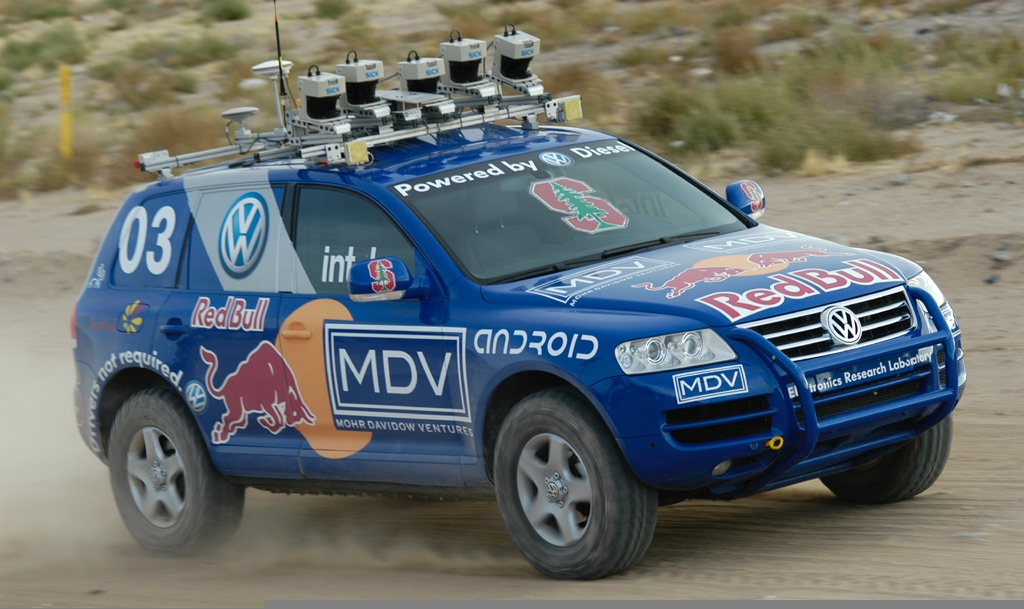
\includegraphics[width=0.5\textwidth]{img/stanley1}
\caption[Stanley]{Stanley, el vehículo autónomo de Stanford que ganó la competencia DARPA Grand Challenge en 2005. 
        Fuente: \href{http://stanford.edu/~cpiech/cs221/apps/driverlessCar.html}{stanford.edu} }
\label{fig:stanley1}
\end{figure}

El éxito de los proyectos que participaron en el grand challenge sentó un gran precedente en el desarrollo de lo que 
ahora se conoce como \textit{Self Driving Car} o vehículo autónomo. De hecho, muchos de los equipos 
participantes de este concurso se constituyen en la actualidad como existosas empresas de desarrollo o 
coadyuvan en iniciativas privadas de gigantes de la tecnología como Google, Uber o Nissan.

Sin embargo, debido al creciente interés tanto en investigación como económico en los sistemas de conducción 
autónoma, la Sociedad de Ingenieros en Automoción (SAE por sus siglas en inglés) ha elaborado un estándar donde se 
detallan distintos aspectos concernientes. La regulación define varios niveles de autonomía en 
vehículos terrestres, aéreos y acuáticos yendo desde un control completamente manual, 
normalmente observado en vehículos completamente mecánicos, pasando por asistencias al control 
hasta llegar a un vehículo completamente autónomo en todas sus tareas

% IMAGEN: niveles de autonomia
%%%% Figura 2 %%%%%%
\begin{figure}[!h] 
\centering
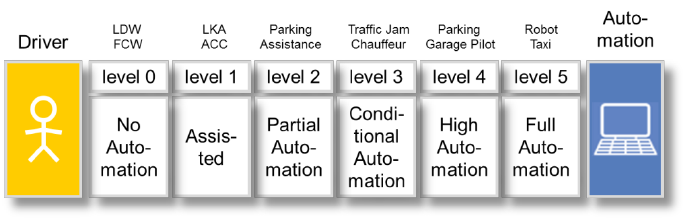
\includegraphics[width=0.70\textwidth]{img/levels}
\caption[Niveles de automatización SAE]{Niveles de automatización en la conducción según SAE. 
        Fuente: \href{https://www.researchgate.net/figure/Terms-related-to-automated-driving-according-to-SAE-and-VDA_fig1_273883061}{researchgate} }
\label{fig:levels}
\end{figure}

La creación de estándares y regulación ha tenido como consecuencia que, en la actualidad, existan varias iniciativas 
en el desarrollo de los \textit{self Driving Cars}, siendo una de las más 
importantes la empresa Waymo, dependiente de Google a través de su empresa Pública Alphabet. Waymo, ha aprovechado 
el uso de tecnologías emergentes de sensado como el LIDAR para mejorar el mapeo y la navegación a través de algoritmos 
de fusión de sensores. Aparte de Alphabet, existen diversas iniciativas privadas en el desarrollo de vehículos autónomos 
con fines comerciales como los Self Driving Cars de Uber, Toyota, BMW, Ford, entre otros.

% IMAGEN: vehiculo de waymo

%%%% Figura 1 %%%%%%
\begin{figure}[!h] 
\centering
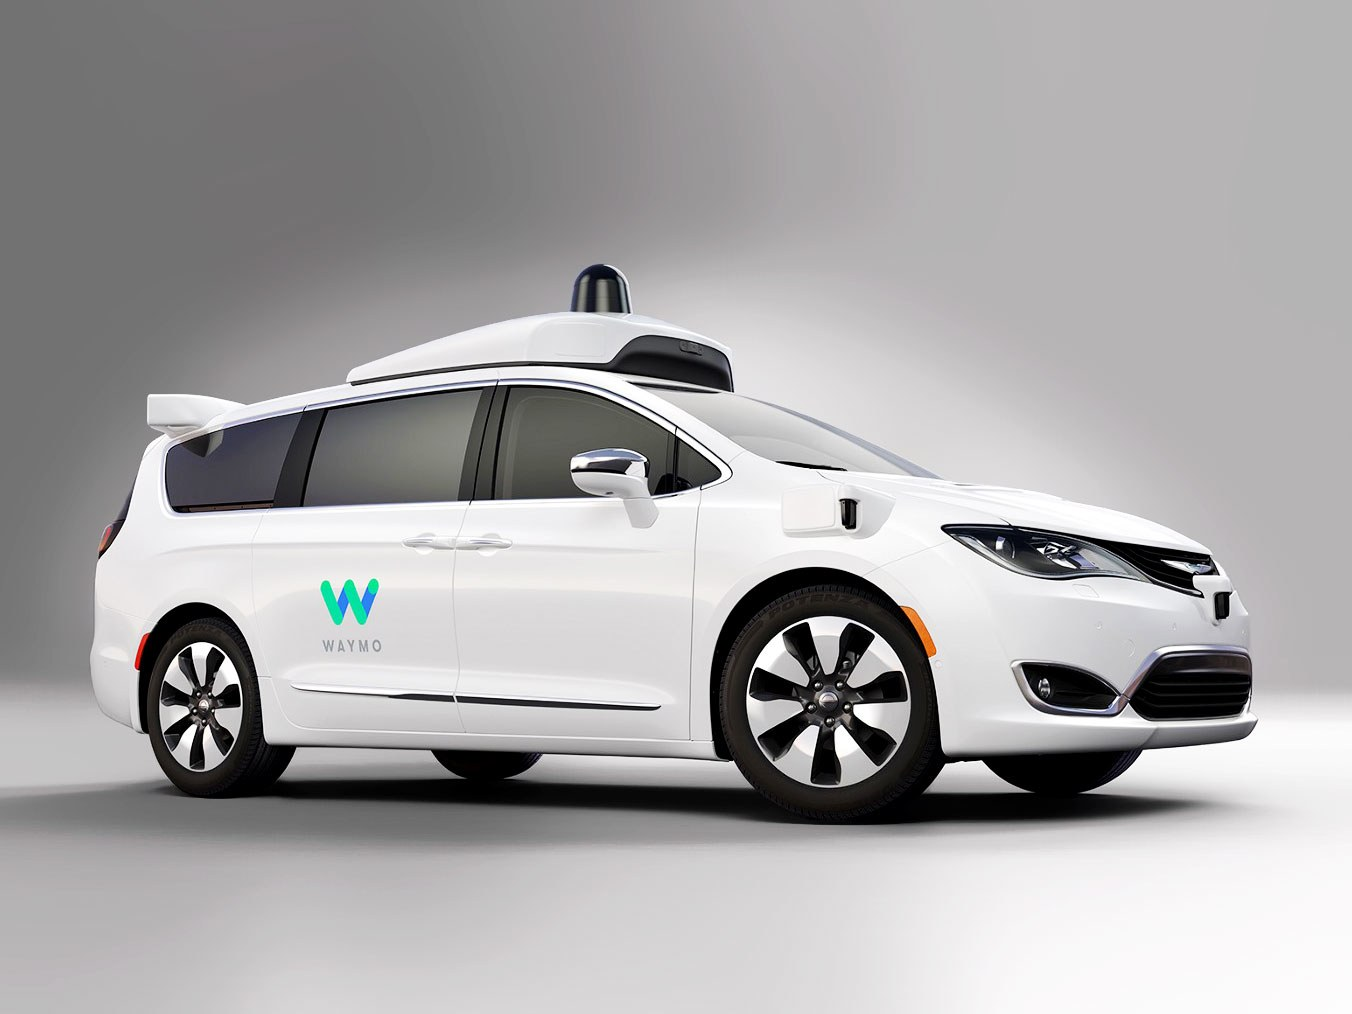
\includegraphics[width=0.5\textwidth]{img/waymo}
\caption[Vehículo de Waymo]{El vehículo autónomo de Waymo. 
        \href{https://waymo.com/}{waymo.com}}
\label{fig:waymo}
\end{figure}

Una de las tareas más importantes dentro de un \textit{self driving car} es la detección y mantención del carril del 
vehículo. Fabricantes de vehículos automotores han incluido con éxito sistemas de asistencia al conductor para la 
mantención del carril usando cámaras digitales y visión artificial para poder detectar la posición del automóvil con 
respecto al carril. Estos sistemas se consideran fundamentales en sistemas de conducción autónoma. Durante las últimas 
dos décadas, se han desarrollado distintos tipos de sistemas y enfoques para resolver el problema de la mantención de 
carril.

\subsubsection{Arquitectura general de un sistema de conducción autónoma}
En general, la arquitectura de un sistema de conducción autónoma se puede entender como la integración de varios módulos o 
subsistemas funcionales que operan en coordinación tal como se puede observar en la Figura(\ref{fig:esquema}). 

% IMAGEN: arquitectura

%%%% Figura 1 %%%%%%
\begin{figure}[!h] 
    \centering
    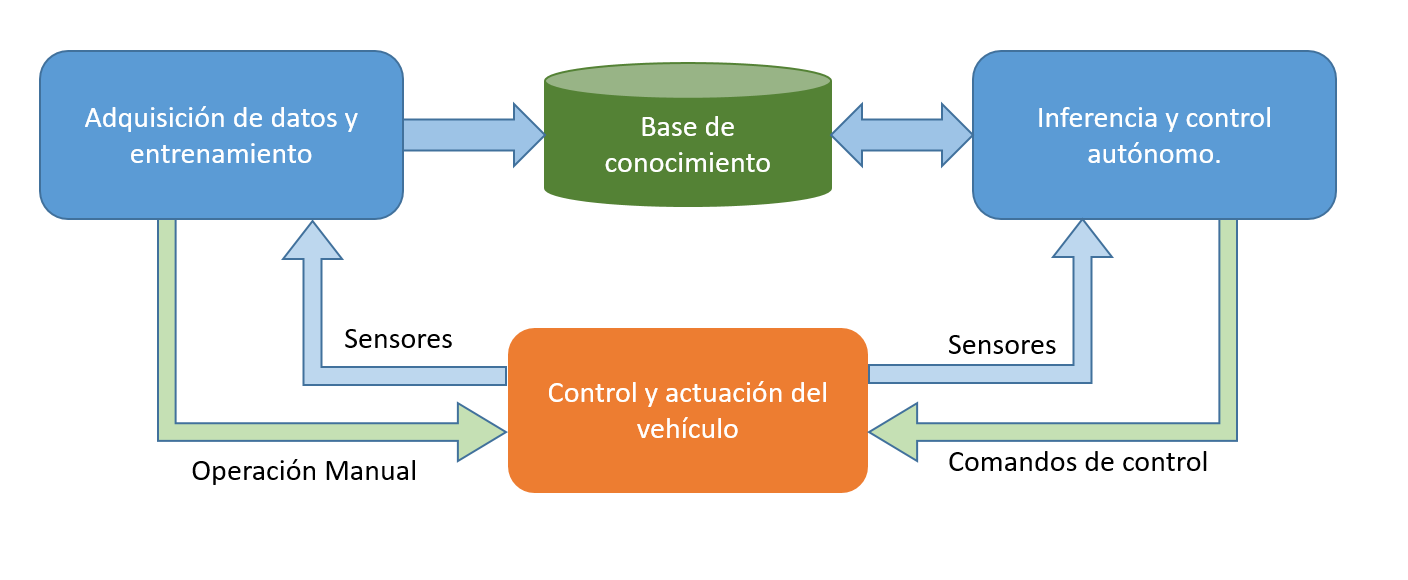
\includegraphics[width=0.75\textwidth]{img/esquema}
    \caption[Arquitectura de un sistema de conducción autónoma]{Arquitectura de un sistema de conducción autónoma. Fuente: Elaboración propia.}
    \label{fig:esquema}
\end{figure}


Normalmente, este tipo de sistemas cuenta con una etapa de adquisición de datos y entrenamiento que servirá para 
alimentar una base de conocimiento o reglas en las que se basará el módulo de inferencia y control autónomo. 
Asimismo, tanto el subsistema de adquisición de datos y entrenamiento como el subsistema de inferencia y 
control autónomo interactuan directamente con el subsistema de control y actuación del vehículo. 

Los mayores esfuerzos se han enfocado principalmente al desarrollo del subsistema de inferencia y 
control autónomo ya que es el que define el rendimiento de un sistema de conducción autónoma en sí. 
Este subsistema, a su vez, puede ser analizado como un conjunto de varios módulos que interactúan 
entre sí de manera secuencial, como se puede apreciar en la Figura(\ref{fig:inferencia}). 

\subsubsection{Sistemas de aprendizaje fin a fin}
Tradicionalmente, los sistemas de aprendizaje requieren de múltiples etapas de procesamiento que interactuan entre sí, como se 
muestra en la Figura(\ref{fig:inferencia}). Por su parte, los sistemas de aprendizaje fin a fin intentan condensar 
estas etapas de procesamiento y reemplazarlas usualmente con una sola red neuronal. Estos sistemas han demostrado ser 
altamente efectivos en contraste a los enfoques tradicionales, principalmente porque abstrae y resumen el diseño de las 
etapas intermedias de un sistema de aprendizaje tradicional con una sola etapa. La desventaja de los 
sistemas de aprendizaje fin a fin radica en la necesidad de grandes cantidades de datos de entrenamiento 
en comparación con los enfoques tradicionales, sin embargo, gracias a la gran disponibilidad de datos de entrenamiento y 
la accesibilidad de instrumentos y herramientas de adquisición de datos, esta desventaja no representa una dificultad de 
gran magnitud en el desarrollo de sistemas fin a fin. 

Los sistemas de aprendizaje fin a fin se han explorado de manera exitosa en los últimos años, esto debido a la creciente
disponibilidad de sistemas de cómputo de alta concurrencia, en especial las Unidades de Procesamiento Gŕafico de propósito
general o GPGPU por sus siglas en inglés. Esta disponibilidad ha logrado que se puedan entrenar redes neuronales completas 
en una estación de trabajo que no consume demasiada energía. Una de las empresas pioneras en GPGPU es Nvidia con su herramienta 
CUDA, que ha permitido el desarrollo de algoritmos de entrenamiento e inferencia para redes neuronales de manera sencilla. Es 
precisamente Nvidia que ha demostrado que los sistemas de aprendizaje fin a fin pueden tener éxito con el desarrollo de un 
prototipo y arquitectura de vehículo autónomo \cite{bojarski2016end}.


%*******************JUSTIFICACION*******************

\section{Justificación del Proyecto}

\subsection{Justificación académica}

Desde el punto de vista académico, el proyecto se justifica en el entendido del uso de técnicas y procedimientos 
de ingeniería para el análisis y diseño de un sistema de aprendizaje “fin a fin” usando redes neuronales y una plataforma 
para el entrenamiento y despliegue del mismo. Tales técnicas y procedimientos incluyen la definición de 
la arquitectura de la red neuronal, el entrenamiento y el análisis del rendimiento de la misma. Así como 
también el dimensionamiento de los componentes de cómputo embebido para el prototipo y la implementación de 
los sistemas de control electrónico de bajo nivel para el mismo. Tales técnicas y 
procedimientos se corresponden de manera integral con los conocimientos adquiridos a lo largo de la carrera 
de Ingeniería Electrónica en sus distintas asignaturas.

\subsection{Justificación tecnológica}

Dada la creciente relevancia de los sistemas autónomos en la actualidad, el proyecto se justifica 
desde el punto de vista tecnológico dado que se presenta la aplicación de nuevas
herramientas y plataformas de software para el desarrollo de sistemas de autónomos, visión por computador 
y redes neuronales convolucionales, que representan áreas vigentes en la investigación tecnológica hoy en día.

El sistema desarrollado se constituirá a su vez en una plataforma de desarrollo sobre el cual se podrá 
extender su funcionalidad y mejorar sus resultados usando herramientas de software de fácil acceso y aprendizaje 
presentando la posibilidad de continuar y extender la investigación en sistemas de conducción autónoma, robótica móvil, 
visión por computador y aprendizaje profundo.

\subsection{Justificación técnica}

Desde el punto de vista de las técnicas aplicadas, el proyecto se justifica dado que se pretende presentar una técnica 
alternativa al enfoque tradicional en el desarrollo de sistemas de aprendizaje, presentando el desarrollo de un sistema 
de aprendizaje fin a fin, que facilitará su análisis, diseño, entrenamiento y puesta en marcha en futuros proyectos 
de investigación y aplicaciones en distintas áreas de la ingeniería. 

La propuesta de la nueva técnica de aprendizaje fin a fin representa un avance en relación al desarrollo de sistemas 
tradicionales por su impacto en el requerimiento de recursos y de conocimiento específico requerido.


%******************ANALISIS DE LA PROBLEMATICA*********************
%------ TODO: completar esta parte ------------- %

\section{Análisis de la problemática y 
planteamiento del problema}
\subsection{Análisis de la problemática}
% PROBLEMATICA: Conjunto de aspectos que causan problemas en un PG.
% ANALISIS DE LA PROBLEMATICA: Determinacion de las causas sus efectos y sus relaciones, vinculados con los aspectos problematicos de la idea del proyecto.  
% ****Es el analisis de las cuestiones discutibles que requieren de una solucion en el PG.

Se han estudiado diferentes enfoques para lograr solucionar la tarea de 
conducción autónoma para vehículos domésticos usando sistemas de aprendizaje. Normalmente, la salida del 
sistema se expresa como una serie de comandos de control de aceleración y dirección 
del volante del vehículo. Estos comandos se pueden obtener de diversas maneras dependiendo 
el nivel de robustez y abstracción que el sistema requiere. Muchos sistemas 
se basan en la fusión de distintos tipos de sensores y fuentes de información como ser 
mapas satelitales, GPS, sensores láser y cámaras. La combinación de esta información 
es procesada y fusionada mediante distintos algoritmos de filtrado tales como el filtro de kalman. 
La característica de este tipo de sistema es que se puede expresar como una serie de etapas 
de procesamiento mediante el cual la información fluye y se transforma, cada una de las etapas es 
diseñada e implementada en base a conocimiento específico y con requerimientos y limitaciones específicas 
de la tarea que realiza tal como se puede apreciar en la Figura(\ref{fig:inferencia}).

Si bien el enfoque anteriormente mencionado ha logrado conseguir importantes avances y resultados 
muy prometedores, involucra un gran esfuerzo a la hora de diseñar cada una de las etapas independientemente 
para luego hacer que funcionen todas juntas y cumplan la tarea asignada. Este proceso usualmente requiere 
de un equipo de expertos que sea capaz de realizar las tareas de diseño de las etapas o módulos del sistema 
y el de la integración de los módulos en un solo sistema funcional. Este enfoque, pese a que ha demostrado ser 
una forma efectiva de trabajo para diversos problemas, tiene la desventaja de requerir muchos 
recursos y tiempo para poder lograr un sistema funcional. 

%
\subsection{Planteamiento del problema} \label{sec:problema}
% PLANTEAMIENTO DEL PROBLEMA: Tiene que ver con enfocar la solucion de los aspectos problematicos tratados, 
% desde su situacion inicial hasta su situacion final deseada.

% definir el concepto de informacion con referencia a datos
% 
De acuerdo a lo establecido anteriormente, se puede considerar a la etapa de inferencia y control autónomo de 
un sistema de conducción autónoma como un sistema de procesamiento de información que consta de varias etapas 
secuenciales que transforman la información de acuerdo a parámetros previamente establecidos. Se debe tener en 
cuenta varios aspectos concernientes tanto al diseño como a la implementación de dichos tipos de sistemas. 

%%%% Figura 1 %%%%%%
\begin{figure}[!h] 
    \centering
    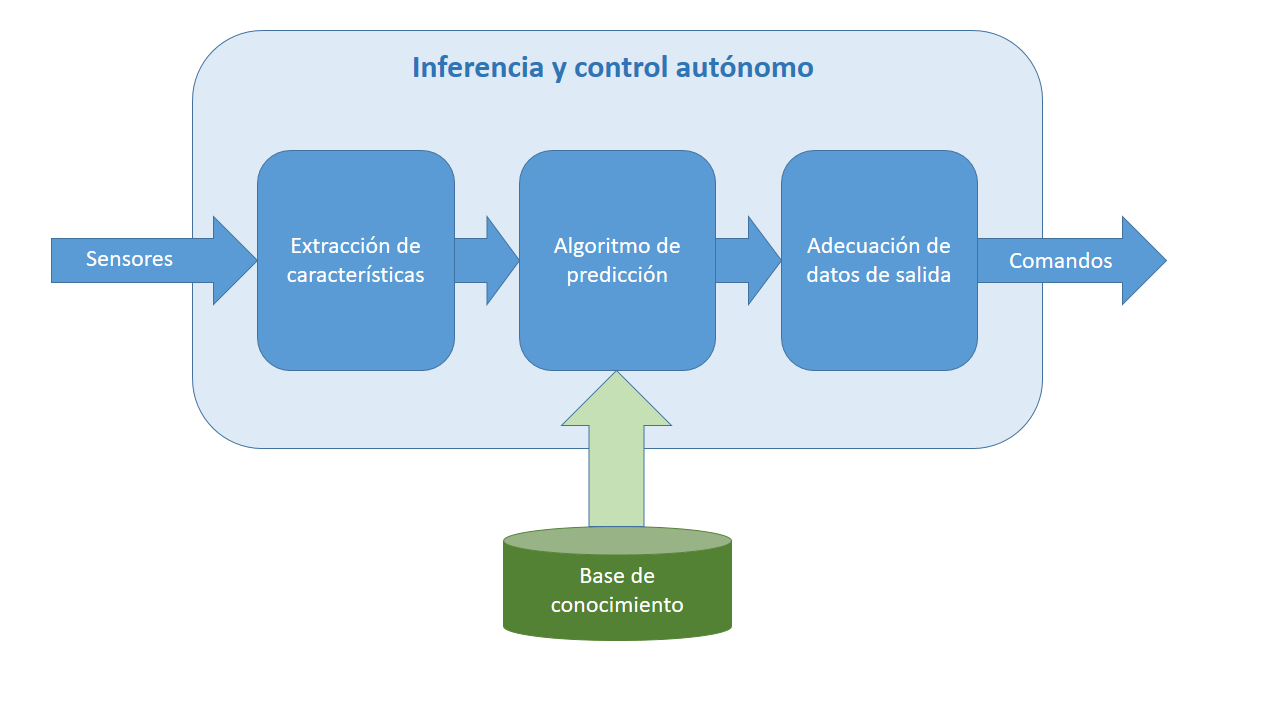
\includegraphics[width=0.75\textwidth]{img/inferencia}
    \caption[Inferencia y control autónomo tradicional]{Componentes del subsistema de inferencia y control autónomo tradicional. Fuente: Elaboración propia.}
    \label{fig:inferencia}
\end{figure}


En el área de visión por computadora para tareas de conducción autónoma, normalmente se sigue el siguiente 
flujo en el desarrollo un sistema o prototipo:

\begin{enumerate}
    \item \textbf{Extracción de características.} Esta etapa incluye el preprocesamiento y transformación de la imagen 
    en un conjunto de características de distinta índole. Estas características se suelen llamar también descriptores 
    y sirven para describir los aspectos más relevantes de la imagen para la tarea final, por ejemplo, la detección de bordes. 
    La extracción de características también se usa para reducir la dimensionalidad inicial de la imagen a una más tratable y 
    amigable con la capacidad de procesamiento computacional disponible. Las características o descriptores a usarse 
    se definen manualmente por medio de conocimiento experto y se afinan de la misma manera.

    \item \textbf{Algoritmo de predicción.} Esta etapa incluye típicamente un algoritmo de aprendizaje previamente 
    entrenado con un conjunto de datos adecuado, permite realizar distintas tareas de alto nivel sobre los descriptores 
    obtenidos de la imagen. Estas descripciones de alto nivel incluyen normalmente tareas de detección, 
    clasificación o regresión. Los algoritmos de aprendizaje incluyen típicamente algoritmos básicos, tales como árboles de decisión,
    regresión lineal o máquinas de soporte vectorial ya que deben realizar la tarea de predicción en un 
    conjunto de dimensionalidad relativamente baja (los descriptores).

    \item \textbf{Adecuación de los datos de salida.} La información extraída de la anterior etapa debe 
    procesarse para poder ser traducida a comandos de control que actuen directamente con las etapas 
    de bajo nivel del vehículo, es decir la etapa de actuación y potencia. En esta etapa se suele incluir algún algoritmo 
    de control realimentado para el control de motores así como también algoritmos de fusión de distintas fuentes de información
    para obtener finalmente una señal de comando para los actuadores.
\end{enumerate}

Como se ha podido observar, el flujo de trabajo en un sistema de conducción autónomo se compone de varias etapas 
secuenciales que se deben realizar con conocimiento y experiencia específica en cada una de las mismas. 

Por su parte, otra de las dificultades con este acercamiento, al reto de la conducción autónoma es el de la reducida
flexibilidad del sistema. En otras palabras, si se quisiera modificar el sistema para agregar requerimientos o 
expandir la funcionalidad del mismo, se debe realizar una modificación a la etapa específica y evaluar el impacto de 
las modificaciones en todo el sistema en su conjunto. Esto dificulta de manera sustancial la reutilización de diversos
componentes en sistemas similares.

Finalmente, la exagerada complejidad y conocimientos requeridos para poder implementar un sistema experimental 
de esta naturaleza hace prácticamente imposible su desarrollo por equipos de investigación pequeños o investigadores 
individuales. Dada la importancia y la potencialidad de los sistemas de conducción autónoma es escencial reducir 
esta dificultad de implementación y experimentación.

En conclusión, el desarrollo de un sistema de conducción autónoma presenta tres principales dificultades a la hora de 
ser abordado: 
\begin{enumerate}
    \item Conocimiento experto de cada una de las etapas involucradas en el sistema.
    \item Poca flexibilidad en el diseño y la implementación del sistema una vez establecido y probado.
    \item El tiempo y recursos necesarios para poder diseñar e implementar un sistema de tal naturaleza lo hace privativo para equipos de investigación pequeños o con poco presupuesto.
\end{enumerate}
%------------------
\section{Objetivos}
\subsection{Objetivo General}

Diseñar un sistema de aprendizaje “fin a fin” capaz de generar de comandos de 
control de vehículos domésticos basado en visión artificial y redes neuronales 
convolucionales para facilitar el diseño e implementación de sistemas de conducción autónoma.

\subsection{Objetivos Específicos}
Para alcanzar el objetivo general será necesario:


\begin{itemize}

    \item Estudiar los aspectos concernientes al desarrollo de sistemas de conducción autónoma y sistemas de aprendizaje.
    \item Analizar los requerimientos de un sistema de conducción autónoma capaz identificar y mantener su carril mientras se conduce.
    \item Diseñar la arquitectura de un sistema de conducción autónoma en base a los requerimientos previamente establecidos.
    \item Diseñar el subsistema de control y actuación para la conducción autónoma de un vehículo con características similares a las de un vehículo doméstico real.
    \item Diseñar el subsistema de adquisición de datos y entrenamiento para tareas de conducción autónoma.
    \item Diseñar el subsistema de inferencia y control autónomo basado en el uso de redes neuronales convolucionales.
    \item Analizar los resultados del entrenamiento e implementación del subsistema de inferencia y control autónomo.
    \item Realizar pruebas de rendimiento y análisis comparativos en el sistema implementado.

\end{itemize}


\section{Alcance}

El presente proyecto de grado cubre los siguientes aspectos dentro de su alcance:

\begin{itemize}
    \item El enfoque del estudio de sistemas de conducción autónomos de vehículos terrestres con el modelo de Ackermann.
    \item Investigación de arquitecturas y plataformas de software para el
    diseño y despliegue de robots móviles y tareas de conducción autónoma.
    \item El desarrollo del sistema se contempla en el marco de un proyecto académico 
    y, por tanto, será implementado usando herramientas de software comúnmente utilizadas en 
    investigación de sistemas autónomos.
\end{itemize}

El alcance detallado previamente estará acotado a su vez por una serie de supuestos.

\section{Límites}
El sistema, por su parte, contará con ciertas restricciones detalladas a 
continuación:
\begin{itemize}
    \item La tarea de conducción autónoma estará enfocada exclusivamente al 
    seguimiento y mantención del carril basado en imágenes provenientes de una cámara 
    sin considerar el reconocimiento e interpretación de otro tipo de información como 
    señales de tránsito, cruces e intersecciones o la presencia de peatones, ciclistas, 
    animales y otros objetos en la ruta.
    \item El prototipo a escala servirá solamente para un análisis superficial 
    de la dinámica de un vehículo automotor doméstico tomando como punto 
    de inicio modelos matemáticos simplificados y limitaciones de rangos de trabajo dentro 
    de dichos modelos.
    \item El diseño de la arquitectura de la red neuronal estará orientado a 
    tareas de aprendizaje supervisado y aproximación de funciones y limitado por la capacidad de 
    procesamiento disponible en el momento de la realización del presente proyecto.
\end{itemize}


\chapter{Marco Teórico} \label{ch:m_teorico}

% estructura
\section{Sistemas de Conducción Autónoma}
Un sistema de conducción autónoma es una combinación de varios componentes o subsistemas donde las tareas 
de percepción, toma de decisiones y operación de un vehículo son desarrolladas por un sistema electrónico en lugar
de un conductor humano. Usualmente, un sistema de conducción autónoma incluye varios subsistemas de automatización 
que operan de manera conjunta y coordinada para poder tomar el control total o parcial del vehículo. 

En algunas ocasiones, la automía del control se implementa de manera condicional, es decir, que el sistema toma 
el control del vehículo para ciertas situaciones pero no todo el tiempo como por ejemplo sistemas de estabilización 
de frenos o prevención de impactos. Este tipo de sistemas se ha ido desarrollando e implementando en vehículos comerciales 
de manera paulatina pero todavía no existe un vehículo completamente autónomo circulando por las calles o carreteras. Notese
que los términos autonomía y automatización se usan de manera intercambiable en este contexto.

Se han desarrollado tres enfoques concernientes al desarrollo de vehículos inteligentes de acuerdo al nivel de autonomía 
que presentan estos sistemas:

\begin{enumerate}
    \item \textbf{Enfoques centrados en el conductor.} Se diseñan en base a la idea de tener a un humano en el lazo de control 
    supervisando las funciones del vehículo
    \item \textbf{Enfoques centrados en una red.} Se diseñan con la idea de que los vehículos inteligentes puedan compartir información entre sí en una infraestructura de red.
    \item \textbf{Enfoques centrados en el vehículo.} Tienen el objetivo de desarrollar vehículos inteligentes completamente autónomos, sin la necesidad de la intervenión de un humano en el lazo de control.
\end{enumerate}

El interés en el desarrollo de vehículos completamente autónomos ha despertado el interés tanto de investigadores en todo 
el mundo así como también de instituciones privadas y gubernamentales que han invertido esfuerzos en fomentar éste desarrollo.
Una de las primeras instituciones en materializar una iniciativa en el desarrollo de vehículos autónomos fue la Agencia de Proyectos 
de Investigación Avanzados (DARPA, por sus siglas en inglés) con el lanzamiento del concurso \textit{Grand Challenge} en el 
año 2003 que era una carrera de vehículos autónomos que debían viajar por más de 200 Km en terrenos escabrosos. Este concurso sin 
sin precedentes atrajo la atención de un número de instituciones de investigación de alto nivel, lo que permitió que el desarrollo 
de este tipo de vehículos diera un gran paso adelante. 

En 2005, una nueva versión del DARPA \textit{Grand Challenge} requirió que los vehículos condujeran por una carretera en un 
desierto. En esta oportunidad, cinco vehículos completaron el trayecto de 211 Km en el desierto, con el vehículo de la Universidad 
de Stanford \textit{Stanley} como ganador, habiendo recorrido todo el trayecto en 6 horas con 54 minutos. En la Figura(\ref{fig:darpa}),
se pueden apreciar fotografías de los vehículos con mejor desempeño en la competencia.

El siguiente hito en el desarrollo de vehículos autónomos, fue el desarrollo del concurso organizado por DARPA 
\textit{Urban Challenge} en el año 2007, en el cual, los vehículos debían cumplir con ciertas tareas de 
navegación pero esta vez en un entorno urbano simulado, con avenidas, intersecciones, señalización y 
otros vehículos circulando simultáneamente. El recorrido comprendía aproximadamente 90 Km y representaba un reto por las 
complejas tareas de decisiones y comportamientos en un entorno de tráfico similar al que se puede encontrar cualquier conductor 
humano conduciendo en una ciudad. En esta ocasión, el ganador de la competencia fue el equipo Tartan Racing, un esfuerzo conjunto entre 
la Carnegie Mellon University y General Motors Corporation con el vehículo Boss, una versión modificada de un Chevrolet Tahoe.


\begin{figure}[!h] 
    \centering
    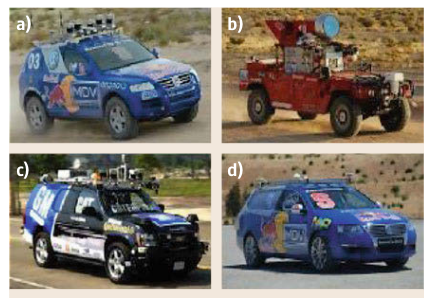
\includegraphics[width=0.75\textwidth]{img/darpa}
    \caption{Vehículos del \textit{Grand Challenge} de 2005: (a) Stanley (1er lugar), (b) Sandstorm (2do lugar). Vehículos del \textit{Urban Challenge} de 2007: (c) Boss (1er lugar) (d) Junior (2do lugar). Fuente: \cite{wikipedia_2018} }
    \label{fig:darpa}
\end{figure}



    \subsection{Niveles de Autonomía SAE}
    Debido al creciente interés e inversión en el desarrolo de sistemas de conducción autónoma se ha establecido 
    una manera de categorizar los niveles de automatización de la conducción por parte de  la Sociedad de Ingenieros en Automoción
    (SAE, por sus siglas en inglés) en la que se definen seis niveles de automatización en vehículos terrestres, acuáticos y aéreos.

        \subsubsection{Nivel 0: Sin automatización}
        El conductor está en completo control de todas las funciones del vehículo en todo momento, no existe intervención 
        de ningún sistema automatizado en el control. Sistemas de alerta de colisión o pérdida de carril entran en esta categoría.
        
        \subsubsection{Nivel 1: Conducción asistida}
        El conductor tiene el control del vehículo, pero el sistema puede modificar la aceleración o dirección del mismo. Los 
        sistemas de control de velocidad de crucero caen en esta categoría.
        
        \subsubsection{Nivel 2: Automatización parcial}
        El conductor debe poder ser capaz de tomar el control del vehículo si ciertas se necesitan ciertas correcciones, pero  
        ya no está en control de la aceleración y dirección del vehículo directamente. Es importante resaltar que desde los
        niveles 0 al 2 el conductor no puede estar distraido en ningún momento de la conducción. Los sistemas de parqueo 
        automático representan un buen ejemplo de sistemas de Nivel 2.
        
        \subsubsection{Nivel 3: Automatización condicional}
        El sistema automatizado tiene el control del vehículo, tanto de la aceleración, dirección así como también del monitoreo 
        del entorno bajo condiciones específicas. El conductor debe estar preparado para intervenir cuando el sistema así lo 
        requiera, por tanto, se permiten distracciones ocasionales. Uno de los sistemas recientemente implementados que cae en esta 
        categoría es el sistema \textit{autopilot} de los vehículos de Tesla Motors. % agregar referencia
        
        \subsubsection{Nivel 4: Automatización elevada}
        El sistema está en completo control del vehículo y la presencia humana ya no es necesaria, sin embargo, la operación autónoma 
        del vehículo está limitada a condiciones específicas. Si las actuales condiciones del entorno sobrepasan las fronteras 
        de rendimiento definidas, el vehículo puede desplegar un protocolo o secuencia de emergencia. Actualmente el desarrollo 
        de vehículos autónomos o \textit{self driving cars} se enfoca en este nivel. 
        
        \subsubsection{Nivel 5: Automatización completa}
        El sistema está en completo control del vehículo y la presencia humana no es necesaria en absoluto. El sistema es capaz 
        de proveer las mismas características que en el Nivel 4, pero en esta ocasión puede operar al vehículo en todas las condiciones.
        En este nivel, el conductor pasa a ser un pasajero en el vehículo. Actualmente, no existen sistemas que operen en este nivel.

    La relación entre la responsabilidad del sistema y el conductor en los distintos niveles se puede apreciar en la 
    Tabla \ref{tbl:niveles}:
    
        \begin{table}[!h]
            \centering
            \resizebox{\textwidth}{!}{%
            \begin{tabular}{@{}|c|l|c|c|c|c|@{}}
            \toprule
            \textbf{Nivel SAE} & \textbf{Denominación}      & \textbf{\begin{tabular}[c]{@{}l@{}}Ejecución de aceleración \\ y dirección\end{tabular}} & \textbf{\begin{tabular}[c]{@{}l@{}}Monitoreo del \\ entorno\end{tabular}} & \textbf{\begin{tabular}[c]{@{}l@{}}Responsable en \\ condiciones difíciles\end{tabular}} & \textbf{\begin{tabular}[c]{@{}l@{}}Modos de \\ conducción\end{tabular}} \\ \midrule
            0                  & Sin Automatización         & Humano                                                                                   & \multirow{3}{*}{Humano}                                                   & \multirow{4}{*}{Humano}                                                                  & Ninguno                                                                 \\ \cmidrule(r){1-3} \cmidrule(l){6-6} 
            1                  & Conducción asistida        & Humano y sistema                                                                         &                                                                           &                                                                                          & \multirow{3}{*}{Algunos Modos}                                          \\ \cmidrule(r){1-3}
            2                  & Automatización parcial     & \multirow{4}{*}{Sistema}                                                                 &                                                                           &                                                                                          &                                                                         \\ \cmidrule(r){1-2} \cmidrule(lr){4-4}
            3                  & Automatización condicional &                                                                                          & \multirow{3}{*}{Sistema}                                                  &                                                                                          &                                                                         \\ \cmidrule(r){1-2} \cmidrule(l){5-6} 
            4                  & Automatización elevada     &                                                                                          &                                                                           & \multirow{2}{*}{Sistema}                                                                 & Varios Modos                                                            \\ \cmidrule(r){1-2} \cmidrule(l){6-6} 
            5                  & Automatización completa    &                                                                                          &                                                                           &                                                                                          & Todos los Modos                                                         \\ \bottomrule
            \end{tabular}%
            }
            \caption{Niveles de automatización según SAE. Fuente: SAE} % TODO: referencia
            \label{tbl:niveles}
            \end{table}

    
    \subsection{Tecnologías requeridas}
    Las tecnologías básicas para sensado y actuación para vehículos autónomos ya existen en el mercado. El reto clave es el 
    de integrar dichas tecnologías con nuevos desarrollos en un sistema estable. Para poder desarrollar sistemas de conducción 
    autónoma confiables y seguros se necesita lo siguiente:

    \begin{itemize}
        \item Una forma de medir o estimar el estado del vehículo.
        \item Una forma de medir o estimar el estado del entorno en el que el vehículo circula.
        \item Acceso a mapas e información satelital.
        \item Una infraestructura de comunicación distribuida con otros vehículos.
    \end{itemize}

        \subsubsection{Estado del vehículo}
        La localización del vehículo es fundamental para tareas de conducción autónoma y debe ser conocida si se desea que siga 
        una trayectoria definida. Para controlar un vehículo de forma que sea capaz de evadir obstáculos o mantener un carril, se 
        necesita conocimiento del estado cinemático y dinámico del mismo. Diversas fuentes de información y datos sobre el estado
        del vehículo pueden ser incorporados como encoders, o unidades inerciales en combinación con medidas de navegación absolutas 
        como GPS. Adicionalmente, la posición del vehículo puede ser conocida con referencia a marcadores locales. Aparte de la 
        localización del vehículo, sistemas de medición de parámetros internos y control de funciones como aceleración, dirección 
        estado del motor, y otros, pueden ser incorporados.

        El desarrollo de modelos adecuados para el control del vehículo también representa una tarea importante pues es en 
        base a estos modelos sobre los cuales se desarrollarán los algoritmos que lo controlen. 

        \subsubsection{Estado del entorno}
        Otro aspecto crítico en el desarrollo de un sistema autónomo es el sensado del estado del entorno y cómo el mismo 
        evoluciona en el tiempo. La tarea más difícil para un vehículo es poder generar un entendimiento de lo que pasa en 
        la carretera, esto incluye poder detectar marcadores clave, otros vehículos, peatones, la carretera o avenida por la que 
        esta circulando actualmente y otros obstáculos como árboles. 
        
        La información se obtiene de diversos tipos de sensores 
        montados en el mismo vehículo, de los cuales los más comunes son los sensores visuales o cámaras que pueden ser posicionadas 
        en distintas orientaciones para poder observar todo lo que ocurre alrededor del vehículo. Los datos de las cámaras 
        son procesados con el objetivo de extraer información valiosa como la ubicación del carril, detección de peatones y otros 
        obstáculos. Otro tipo de sensores utilizados comunmente son sensores de proximidad, que permiten obtener medidas de distancia 
        a los obstáculos más cercanos ofreciendo así información al vehículo sobre su posición relativa a los mismos. 
        
        Un tipo especial de sensores muy comunes en vehículos autónomos son los LIDAR, que generan una nube de puntos 
        con información acerca de la distancia a los obstáculos más cercanos en dos y tres dimensiones.
        % imagen de lidar 
        \begin{figure}[!h] 
            \centering
            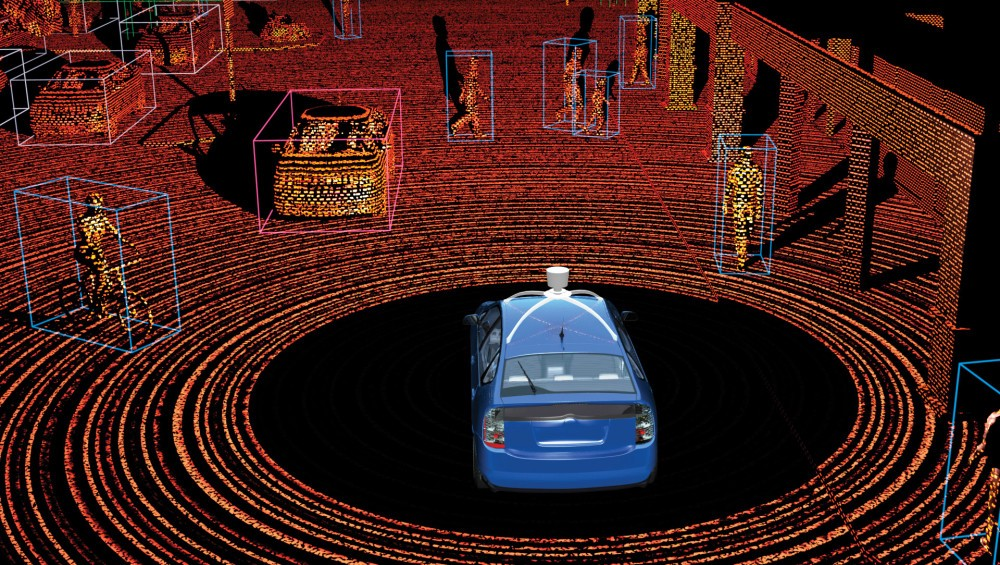
\includegraphics[width=0.75\textwidth]{img/lidar}
            \caption{Visualización de los datos provenientes de un LIDAR para tareas de conducción autónoma. Fuente: \cite{cameron_2017} }
            \label{fig:lidar}
        \end{figure}
        

    \subsection{Arquitectura de un sistema de conducción autónoma}
    En base a los distintos aspectos detallados anteriormente (Figura(\ref{fig:esquema})), en el marco de los objetivos del presente 
    proyecto, se puede describir a la tarea de conducción autónoma usando una arquitectura compuesta 
    por tres elementos o subsistemas fundamentales: el subsistema de control y actuación del vehículo, el 
    subsistema de adquisición de datos y entrenamiento y el subsistema de inferencia y control.

        \subsubsection{Subsistema de control y actuación.}
        Este subsistema representa la parte física y de bajo nivel del vehículo, el vehículo en sí, 
        sumado a los sistemas de control y sensado incorporados. Este subsistema cuenta con las interfaces necesarias 
        para controlar el vehículo mediante comandos de control de aceleración y dirección y con los medios 
        para extraer información del estado interno del vehículo, así como también del entorno con cámaras o sensores 
        de proximidad. Por sí solo, este subsistema no es capaz de realizar ninguna tarea de conducción autónoma.

        % TODO: grafico del subsistema
        \subsubsection{Subsistema de adquisición de datos y entrenamiento.}
        Este subsistema se compone de un conjunto de herramientas y utilidades para la 
        adquisición de conjuntos de datos de entrenamiento y validación, así como
        también un módulo de entrenamiento de la red neuronal convolucional para la tarea de
        la generación de comandos de control. En la parte de adquisición de datos, provee de las herramientas necesarias 
        para poder extraer información relevante de sesiones de conducción controlada por un operador humano de forma 
        que se tengan los datos necesarios para que el vehículo pueda aprender la forma de conducir en base a una referencia 
        de conducción humana.

        \subsubsection{Subsistema de inferencia y conducción autónoma.}
        El subsistema de inferencia y conducción autónoma tiene la tarea de obtener y ejecutar
        las predicciones del modelo predictivo entrenado en el Subsistema de Adquisición de Datos y Entrenamiento.
        Este subsistema tomará como entradas los datos de los 
        sensores a bordo del vehículo para generar comandos de control acordes con el entorno
        percibido. Este subsistema usualmente está implementado en forma de un programa de ``piloto automático''
        capaz de conducir el prototipo de manera autónoma de acuerdo a las limitaciones definidas en el diseño.

\section{Visión Artificial}
La visión es un sentido fundamental en el desarrollo de cualquier persona y, entender el entorno basados en la información que 
un humano puede ver es relativamente sencillo. Tareas como reconocer la forma y color de un objeto cercano o contar las personas 
presentes en una fotografía de grupo son tareas triviales para un ser humano. La visión artificial es un campo de 
las ciencias de la computación que intenta reproducir las capacidades de una persona para entender imágenes. Este campo
aglutina técnicas matemáticas para recuperar la forma y apariencia en tres dimensiones de objetos en una imagen. Se trata 
del desarrollo de distintas técnicas y algoritmos que intentan recuperar la información más importante de una imagen digital, 
en otras palabras, que una computadora pueda entender una imagen. En la actualidad, las técnicas de visión artificial son 
usadas en diversas aplicaciones de la vida real de las cuales podemos citar algunas:

\begin{itemize}
    \item \textbf{Reconocimiento optico de caracteres (OCR):} Lectura de dígitos manuscritos de códigos postales (Figura(\ref{fig:cvision}a)) y reconocimiento automático de placas de vehíchulos.
    \item \textbf{Inspección automática:} Inspección de partes para el control de calidad en líneas de producción industriales(Figura(\ref{fig:cvision}b)).
    \item \textbf{Ventas:} Reconocimiento de objetos para pagos en cajas automatizadas(Figura(\ref{fig:cvision}c)).
    \item \textbf{Reconstrucción de modelos en 3D (fotogrametría):} Reconstrucción automática de modelos en tres dimensiones a partir de fotografías aéreas.
    \item \textbf{Imagenología médica:}  Registro de imágenes pre y post operatorias para estudios y diagnósticos especializados(Figura(\ref{fig:cvision}d)).
    \item \textbf{Seguridad automotriz:} Detección de obstáculos inesperados como peatones o ciclistas en situaciones donde métodos convencionales de detección de obstáculos no pueden aplicarse (Figura(\ref{fig:cvision}e)).
    \item \textbf{Seguridad y vigilancia:} Monitoreo de actividad sospechosa y análisis de tráfico en carreteras (Figura(\ref{fig:cvision}f)).
\end{itemize}


\begin{figure}[!h] 
    \centering
    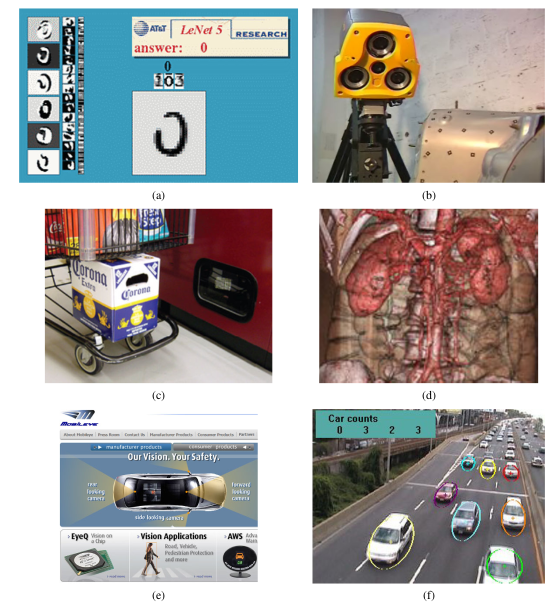
\includegraphics[width=0.75\textwidth]{img/cvision}
    \caption{Algunas aplicaciones de la visión artificial. Fuente: \cite{Szeliski2011} }
    \label{fig:cvision}
\end{figure}

    \subsection{Caracterización de una imagen digital}
    Luego de surgir de una o más fuentes de luz, reflejarse de una o más superficies y pasar a través del lente de una cámara, 
    la luz finalmente llega al sensor óptico. Los fotones incidentes en el sensor son convertidos en valores de intensidad de 
    color rojo, verde y azul (RGB) en un arreglo matricial que es lo que se conoce como una imagen digital. Todas las etapas 
    envueltas en la obtención de una imagen digital se pueden apreciar en la Figura(\ref{fig:digitalcam}) donde se diferencian 
    dos subproductos del proceso de conversión: la imagen \textit{raw} y la imagen compresa. Esta diferenciación nace de la 
    necesidad de representar imágenes digitales sin ocupar mucho espacio en la memoria y para poder comprimir una imagen 
    \textit{raw} se realizan varios procesos complementarios.

    \begin{figure}[!h] 
        \centering
        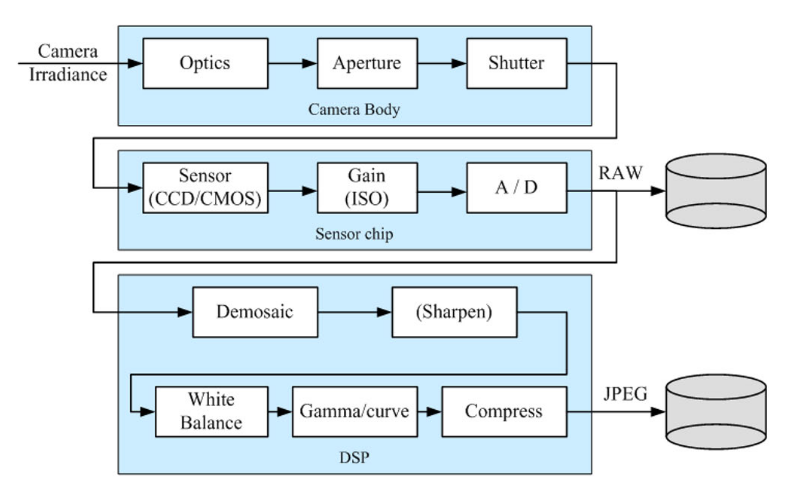
\includegraphics[width=0.75\textwidth]{img/digitalcam}
        \caption{Proceso de la obtención de una imagen con una cámara digital. Fuente: \cite{Szeliski2011} }
        \label{fig:digitalcam}
    \end{figure}

    El sensor óptico se compone de un arreglo bidimensional de pixeles sensibles a la luz y a ciertos rangos de longitud de onda de 
    la luz, lo que significa que pueden detectar ciertos colores o características de la luz que incide en ellos. Este arreglo 
    se transforma en una matriz con valores de intensidad para cada color en cada pixel, es así como se puede entender 
    a una imagen digital como un arreglo multidimensional de valores. 

    \begin{figure}[!h] 
        \centering
        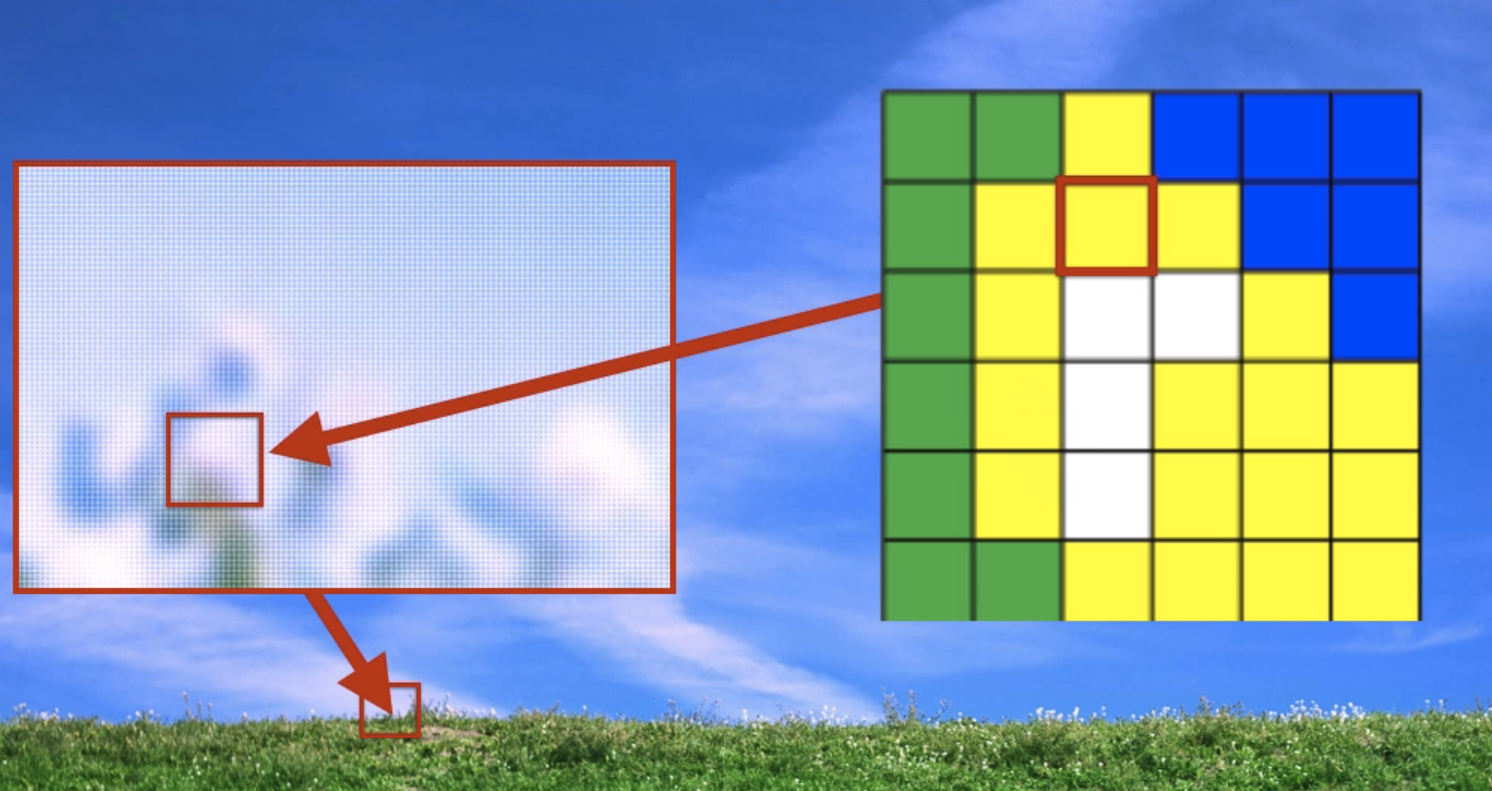
\includegraphics[width=0.75\textwidth]{img/digitalimg}
        \caption{Representación de una imagen digital como un arreglo de pixeles. Fuente: \cite{Szeliski2011} }
        \label{fig:digitalimg}
    \end{figure}

    La tarea de la visión artificial es especialmente complicada pues se intenta dar sentido o significado a un arreglo bidimensional 
    de pixeles. Existen distintos métodos y algoritmos que intentan convertir esta inmensa cantidad de datos (los pixeles) en 
    información útil (objetos).

\section{Redes Neuronales Artificiales}         %done

    \subsection{Aprendizaje Automático}
    El aprendizaje automático es un subcampo de la inteligencia artificial que intenta extraer 
    patrones mediante un proceso de \textit{aprendizaje} a partir de datos \cite{Mitchell1990}. Este proceso 
    de aprendizaje se define de acuerdo a una \textbf{tarea específica} $T$ que intenta aprenderse en base 
    a \textbf{experiencia pasada} $E$ tomando como referencia una \textbf{medida de rendimiento} $P$ . 
    Dentro de esta definición, se puede listar varios ejemplos de tareas de aprendizaje que usualmente se resuelven  
    usando los conceptos del aprendizaje automático o también llamado \textit{machine learning}:
    \\
    \\
    \begin{itemize}
        \item \textbf{Un algoritmo de aprendizaje que pueda jugar ajedrez:}
        \begin{itemize}
            \item \textbf{Tarea $T$:} Jugar Ajedrez.
            \item \textbf{Medida de Rendimiento $P$:} Porcentaje de partidas ganadas contra el oponente.
            \item \textbf{Experiencia $E$:} Información de varias partidas de práctica.
        \end{itemize}
        
        \item \textbf{Un algoritmo de aprendizaje que pueda reconocer dígitos manuscritos:}
        \begin{itemize}
            \item \textbf{Tarea $T$:} Reconocer y clasificar dígitos manuscritos dentro de una imagen.
            \item \textbf{Medida de Rendimiento $P$:} Porcentaje de dígitos correctamente clasificados.
            \item \textbf{Experiencia $E$:} Base de datos de imágenes de dígitos con sus etiquetas correspondientes.
        \end{itemize}

        \item \textbf{Un algoritmo de aprendizaje que pueda reconocer la voz:}
        \begin{itemize}
            \item \textbf{Tarea $T$:} Extraer una secuencia de palabras de una grabación de voz.
            \item \textbf{Medida de Rendimiento $P$:} Porcentaje de palabras correctamente predichas.
            \item \textbf{Experiencia $E$:} Grabaciones de voz con una transcripción correspondiente.
        \end{itemize}
    
    \end{itemize}
    

    Esta definición de aprendizaje es lo suficientemente amplia como para englobar todas las tareas 
    que el campo del aprendizaje automático intenta resolver en la actualidad. Sin embargo, debido a 
    su naturaleza, se pueden clasificar las tareas de aprendizaje en tres grandes categorías que tienen
    características particulares: aprendizaje supervisado, aprendizaje no supervisado y aprendizaje por refuerzo.

    La diferencia entre estos tres tipos de problemas surge de la distinta naturaleza de la experiencia $E$ disponible
    para el entrenamiento. A continuación, se procede a detallar cada uno de ellos.

        \subsubsection{Aprendizaje supervisado} \label{sss:supervisado}
        En el caso de las tareas de aprendizaje supervisado, la experiencia constituye un conjunto de datos o \textit{dataset}
        que contiene ejemplos con \textit{características} y cada ejemplo está asociado con una \textit{etiqueta}. Por ejemplo, 
        un conjunto de datos de flores donde cada registro contiene datos de la flor (características) y la especie a la que pertenece (etiqueta). 
        Dentro de los algoritmos que atacan problemas de aprendizaje supervisado se pueden encontrar 2 grandes categorías.
            \paragraph{Clasificación}
            Las tareas de clasificación tienen como característica el hecho de que la etiqueta de cada ejemplo en el 
            conjunto de datos pertenece a una categoría o, en otras palabras, tiene una naturaleza discreta y finita. Por ejemplo, 
            en el caso de la clasificación de las flores mencionado anteriormente, la etiqueta solamente puede pertenecer a un
            conjunto finito de especies de flores y cada ejemplo pertenece a una de estas especies.
            \paragraph{Regresión}
            En las tareas de regresión, las etiquetas pertenecen a un conjunto de números reales o de naturaleza 
            contínua. En este caso, las etiquetas no se asocian con categorías sino más bien con otro tipo de variables. Un 
            ejemplo muy conocido es el de la tarea de la predicción del precio de una casa en base a sus características, el precio 
            de una casa no puede categorizarse porque representa un número que puede tener infinitos valores dentro de un rango definido.
        

            \begin{figure}[!h] 
                \centering
                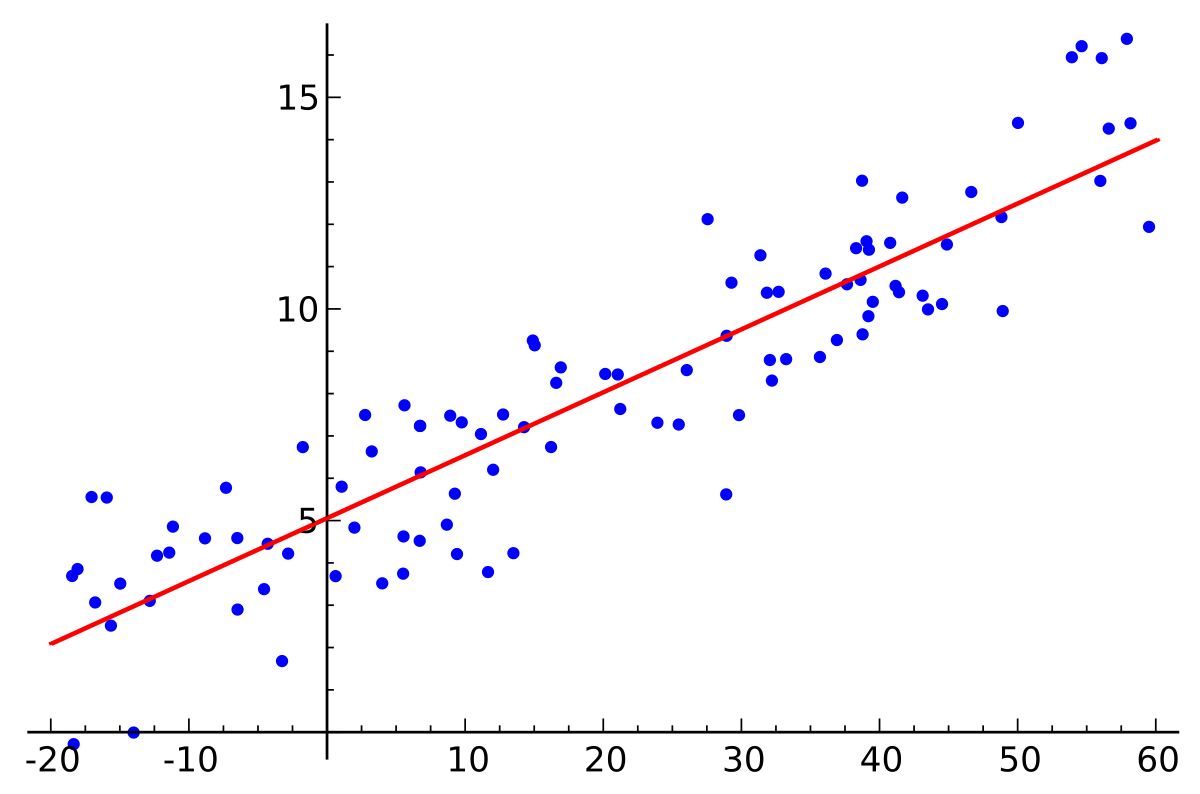
\includegraphics[width=0.75\textwidth]{img/regression}
                \caption{Regresión lineal, una tarea de aprendizaje supervisado. Fuente: \cite{wikipedia_2018} }
                \label{fig:regresion}
            \end{figure}

        En las tareas del aprendizaje supervisado, se puede considerar cada ejemplo como una descripción de 
        una situación (características) en conjunto con una especificación (etiqueta), cada uno de los ejemplos 
        dentro el conjunto de datos son eventos independientes y se pueden analizar por separado. En este sentido
        la tarea del algoritmo es generalizar la respuesta para casos no presentes en el conjunto inicial de datos.

        \subsubsection{Aprendizaje no supervisado}
        En las tareas del aprendizaje no supervisado la experiencia contenida en el conjunto de datos tiene la característica de 
        no poseer ninguna etiqueta, por tanto, usualmente se intenta buscar una estructura escondida dentro el conjunto de datos 
        o, dicho de otra manera, se buscan patrones que puedan presentarse en dichos datos. Estos patrones pueden aprovecharse 
        para extraer información relevante de la naturaleza de datos de muy alta dimensionalidad, información que normalmente no 
        es trivial de encontrar o visualizar por una persona. Entre algunas de las tareas más comunes dentro del aprendizaje no 
        supervisado, se pueden listar:

            \paragraph{Clustering}
            Refiere a la tarea de separar y agrupar los datos en un número finito de conjuntos o \textit{clusters}. Los 
            \textit{clusters} normalmente denotan una estructura oculta dentro de los datos y proporcionan información acerca 
            de la similaridad entre ejemplos del conjunto de datos.

            \begin{figure}[!h] 
                \centering
                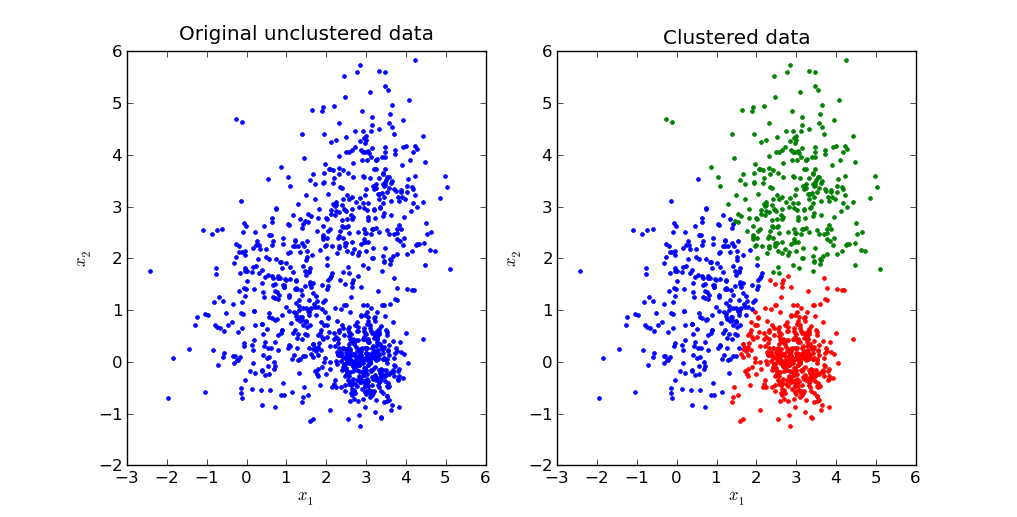
\includegraphics[width=0.75\textwidth]{img/clustering}
                \caption{Clustering, una tarea de aprendizaje no supervisado. Fuente: \cite{viswarupan_2017} }
                \label{fig:clustering}
            \end{figure}

            \paragraph{Reducción de dimensionalidad}
            Uno de los problemas con las bases de datos y conjuntos de datos disponibles es que poseen una dimensionalidad 
            bastante alta haciendo prácticamente imposible para un humano poder visualizar o encontrar patrones e información 
            útil en los mismos. Este problema se suele tratar con algoritmos de reducción de dimensionalidad, en la que 
            se encuentra una representación estimada de los datos pero con menos dimensiones. Uno de los algoritmos más 
            conocidos y usados en esta categoría es el análisis de componente principal o PCA, por sus siglas en inglés, en el 
            que se encuentra una representación de los datos en una menor dimensión usando proyecciones ortogonales.

            \paragraph{Estimación de probabilidad}
            Muchos conjuntos de datos son obtenidos de distintas fuentes y a lo largo de varios intervalos de tiempo, en este 
            entendido, es muy útil conocer o aproximar la distribución de probabilidad de los datos para luego poder realizar 
            predicciones o tratarlos con algún modelo en específico.

        \subsubsection{Aprendizaje por refuerzo}
        En las tareas de aprendizaje por refuerzo se toma en cuenta la interacción de un agente con su entorno y la forma 
        en la que las acciones que toma dicho agente afectan a su entorno y se materializan en una recompensa o castigo \cite{sutton2018reinforcement}. Formalmente
        se pueden definir ciertos elementos que componen una tarea de aprendizaje por refuerzo:
        \begin{itemize}
            \item \textbf{Agente.} Es la entidad que interactúa con el entorno. El agente se comunica con el entorno mediante acciones.
            \item \textbf{Política.} Representan la forma de actuar del agente en base al conocimiento que ha adquirido.
            \item \textbf{Recompensa.} Es la función que define la efectividad del agente de cumplir el objetivo deseado, normalmente, el aprendizaje se enfoca en maximizar la recompensa que el agente puede obtener. 
        \end{itemize}
        
        \begin{figure}[!h] 
            \centering
            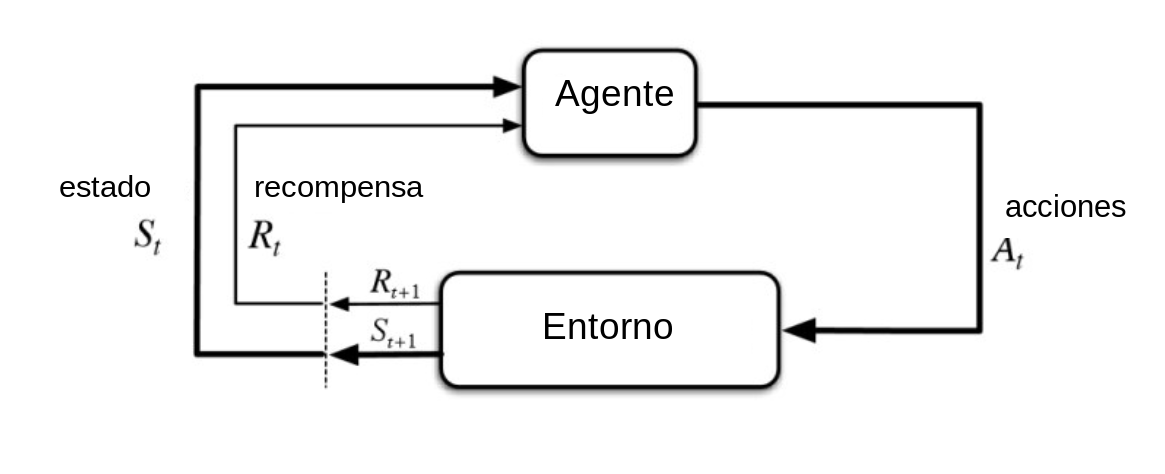
\includegraphics[width=0.75\textwidth]{img/refuerzo}
            \caption{Esquema de una tarea de aprendizaje por refuerzo. Fuente: \cite{bhatt_2018} }
            \label{fig:refuerzo}
        \end{figure}

        
    \subsection{Aprendizaje Profundo}
    Dentro del campo de la inteligencia artificial y el aprendizaje automático se han implementado diversos tipos 
    de algoritmos con éxito en los tipos de tareas de aprendizaje mencionados anteriormente. La base teórica y los detalles 
    de implementación de estos algoritmos son muy variados, sin embargo, las redes neuronales artificiales han experimentado 
    un incremento en el interés en la investigación y en las aplicaciones muy importante. Tal es el éxito de las mismas 
    que se ha creado un subcampo exclusivo llamado aprendizaje profundo o \textit{deep learning}. El aprendizaje profundo 
    es un campo de la inteligencia artificial que se encarga de estudiar exclusivamente a las redes neuronales artificiales, 
    sus componentes, arquitectura y aplicaciones. El impresionante rendimiento de estos algoritmos reside principalmente en el 
    concepto de la representación que generan a partir de los datos que se procesan. 

    El aprendizaje profundo resuelve el problema del aprendizaje de representaciones al introducir representaciones que se 
    expresan en términos de otras representaciones más simples. Además, permite a una computadora construir conceptos complejos 
    a partir de conceptos más simples. Un ejemplo de la generación de estos conceptos o representaciones se puede apreciar en la 
    Figura(\ref{fig:representacion}).
    
    
    \begin{figure}[!h] 
        \centering
        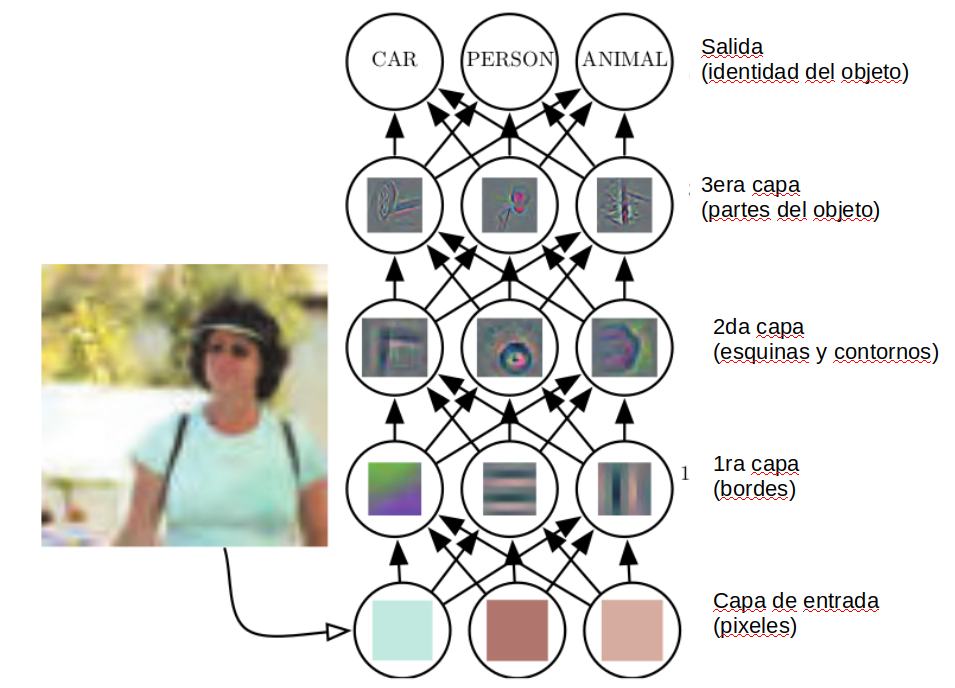
\includegraphics[width=0.75\textwidth]{img/representacion}
        \caption{Ilustración de un modelo de aprendizaje profundo. Las representaciones se generan en las capas ocultas y corresponden con características de distintos niveles de complejidad. Fuente: \cite{Goodfellow-et-al-2016} }
        \label{fig:representacion}
    \end{figure}

    A continuación, se procede a definir los conceptos más importantes de redes neuronales artificiales con los cuales se podrá 
    plantear la solución al problema de la conducción autónoma usando visión artificial.

        \subsubsection{Redes neuronales feedforward}
        Las redes neuronales feedforward o también llamadas perceptrón multicapa, son la base fundamental de los modelos 
        de aprendizaje profundo. El objetivo de una red neuronal feedforward es el de aproximar una función $f^\ast$. Por 
        ejemplo, para una tarea de clasificación, $y = f^\ast (\mathbf{x})$ mapea una entrada $\mathbf{x}$ a una categoría $y$.
        Una red neuronal feedforward define un mapeo $\mathbf{y} = f(\mathbf{x},\mathbf{W})$ y aprende el valor de los parámetros 
        $\mathbf{W}$ que resulten en la mejor aproximación\cite{Goodfellow-et-al-2016}.

        Este tipo de modelos son denominados feedforward debido a que la información fluye a por la función siendo evaluada 
        desde $\mathbf{x}$, a través de distintos cálculos intermedios definidos por $f$, hasta llegar a la salida $\mathbf{y}$.
        No existen conexiones de retroalimentación en las que la salidas del modelo se inyecten de nuevo a sí mismo. Las redes 
        neuronales que poseen este tipo de conexiones de retroalimentación son denominadas redes neuronales recurrentes.

        Para definir una red neuronal feedforward se puede comenzar definiendo un modelo basado en una combinación 
        lineal en conjunto con una función no lineal que toma la siguiente forma:

        \begin{equation}\label{eq:modelobase}
            y(\mathbf{x}, \textbf{W}) = f\left(\sum_{j=1}^M w_j  x_j\right)
        \end{equation}

        donde $f()$ es una función de activación no lineal. Esto lleva al modelo básico de una red neuronal que puede ser 
        descrita como una serie de transformaciones. Primero, se construyen $M$ combinaciones lineales de las variables 
        de entrada $x_1, \ldots , x_D$ donde $D$ es la dimensión del vector de entrada $\mathbf{x}$:
        
        \begin{equation}
            a_j = \sum_{i=1}^D w_{ji}^{(1)} x_i + w_{j0}^{(1)}
        \end{equation}

        donde $j = 1, \ldots , M$, y el superíndice $(1)$ indican que los correspondientes parámetros se encuentran en la 
        primera capa de la red. Los parámetros $w_{ji}^{(1)}$ se suelen conocer también con el nombre de \textit{pesos} y 
        los parámetros $ w_{j0}^{(1)}$ con el nombre de \textit{sesgos} o \textit{biases}. Las cantidades $a_j$ se conocen 
        como \textit{activaciones}, y cada una de ellas es luego transformada usando una función no lineal y derivable conocida 
        como la \textit{función de activación} $h()$ para luego obtener:

        \begin{equation}
            z_j = h(a_j)
        \end{equation}

        Estas cantidades corresponden con la salida de la capa y también se suelen referir por el nombre de  \textit{unidades ocultas}.
        Las funciones no lineales $h()$ pueden escogerse dependiendo a diversos criterios de rendimiento o de comportamiento. Siguiendo
        a la Ecuación(\ref{eq:modelobase}), las unidades ocultas se pueden volver a procesar con una combinación lineal y función 
        de activación en una segunda capa:

        \begin{equation}
            a_k = \sum_{j=1}^M w_{kj}^{(2)} z_j + w_{k0}^{(2)}
        \end{equation}

        donde $k = 1, \ldots, K$ y $K$ corresponden con el número de salidas de la segunda capa. Finalmente, si se considera a 
        esta capa como la capa de salida, podemos transformar las activaciones de la segunda capa con una función de activación. 
        Normalmente, para una tarea de regresión, la función de activación es una función identidad, es decir $y_k = a_k$. Para 
        una tarea de clasificación binaria, en cambio, la función de activación es una función sigmoide:

        \begin{equation}
            y_k = \sigma(a_k)
        \end{equation}

        donde
        
        \begin{equation}\label{eq:sigmoide}
            \sigma(a) = \frac{1}{1 + e^{-a}}    
        \end{equation}
        
        Finalmente, se pueden combinar las etapas en una función general de la red que, para una salida sigmoidal, toma la 
        siguiente forma:

        \begin{equation}\label{eq:reddoscapas}
            y_k(\mathbf{x}, \mathbf{W}) = \sigma \left( \sum_{j=1}^M w_{kj}^{(2)} h \left( \sum_{i=1}^D w_{ji}^{(1)} x_i + w_{j0}^{(1)} \right) + w_{k0}^{(2)} \right)
        \end{equation}

        De esta manera, se define una red neuronal de dos capas a partir de la combinación lineal de las entradas y las unidades 
        ocultas con los parámetros o pesos de la red transformados por funciones de activación no lineal. La arquitectura de la 
        red definida en la Ecuación(\ref{eq:reddoscapas}) se puede visualizar en la Figura(\ref{fig:reddoscapas}) donde se observa claramente las relaciones que se 
        han definido anteriormente en forma gráfica y la naturaleza del flujo en una sola dirección (feerforward) de los datos 
        desde la entrada hasta la salida. En este caso, la red neuronal analizada es una red neuronal con una capa oculta.

        \begin{figure}[!h] 
            \centering
            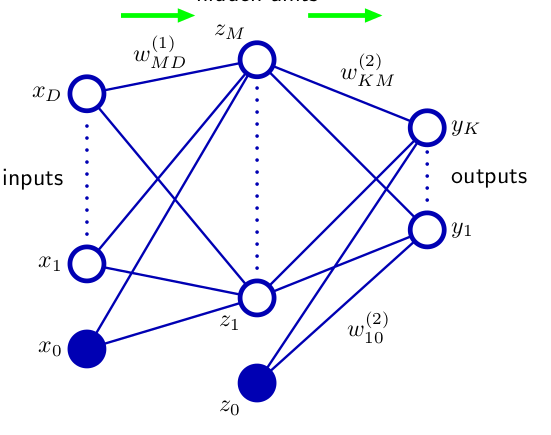
\includegraphics[width=0.75\textwidth]{img/reddoscapas}
            \caption{Diagrama de la red neuronal de dos capas correspondiente a la Ecuación(\ref{eq:reddoscapas}). Fuente: \cite{Bishop2006} }
            \label{fig:reddoscapas}
        \end{figure}
        
        \subsubsection{Funcion de costo}
        La función de costo es una función que permite definir el rendimiento de una red neuronal con respecto a las 
        predicciones esperadas a la salida. Un aspecto importante en el diseño de una red neuronal es la elección adecuada 
        de la función de costo. 

        La función de costo o función de error, se define de manera similar al caso del ajuste de curvas. Es decir, se desea 
        minimizar una suma de errores cuadráticos. Dado un conjunto de entrenamiento compuesto por un conjunto de vectores 
        de entrada $\{\mathbf{x}_n \}$, donde $n = 1, \ldots , N$, junto con un conjunto de vectores objetivo $\{\mathbf{t}_n \}$
        el objetivo es minimizar la función:

        \begin{equation}\label{eq:error}
            E(\mathbf{w}) = \frac{1}{2} \sum_{n=1}^N \{y(\mathbf{x}_n, \mathbf{w}) - t_n\}^2
        \end{equation}

        donde el valor de $\mathbf{w}$ que minimice la función de error $E(\mathbf{w})$ será considerado como el mejor conjunto 
        de parámetros sobre el cual el modelo puede generalizar.

        \subsubsection{Entrenamiento usando gradientes y retropropagación} \label{sec:gradientes}

        Una vez definidos con claridad los componentes básicos de una red neuronal feedforward y cómo es el proceso del flujo 
        de la información desde la entrada $\mathbf{x}$ hasta la salida $\mathbf{y}$, solamente queda especificar el procedimiento 
        necesario para ajustar los parámetros o pesos de la red $\mathbf{W}$. Para este cometido, el método más usado es el 
        de la retropropagación o \textit{backpropagation}, popularizado a partir del paper de Rumelhart \cite{rumelhart1986learning} 
        y ampliamente usado en la actualidad en la mayoría de las redes neuronales. La retropropagación tiene el objetivo de 
        encontrar los gradientes, en específico, se desea encontrar el gradiente de de la función de costo o error con respecto 
        a los parámetros $\nabla_{\mathbf{W}}E(\mathbf{W})$. Si se toma en cuenta que una red neuronal feedforward puede tener 
        varias capas ocultas, la gradiente de la función de costo está en función de los parámetros y funciones de activación 
        de cada capa, por tanto, se necesita usar la regla de la cadena para poder encontrar estos gradientes intermedios.

        Sea $y = g(x)$ y $z = f(g(x)) = f(y)$ dos funciones reales con argumento real, la regla de la cadena define lo siguiente:

        \begin{equation}
            \frac{dz}{dx} = \frac{dz}{dy} \frac{dy}{dx}
        \end{equation}

        Se puede generalizar la anterior expresión para casos fuera de una variable escalar donde $x \in \mathbb{R}^m$, 
        $y \in \mathbb{R}^n$, $g$ mapea de $\mathbb{R}^m$ a $\mathbb{R}^n$ y $f$ mapea de $\mathbb{R}^m$ a $\mathbb{R}$,
        si $\mathbf{y} = g(\mathbf{x})$ y $\mathbf{z} = g(\mathbf{y})$, entonces:

        \begin{equation}
            \frac{dz}{dx_i} =\sum_j \frac{dz}{dy_j} \frac{dy_j}{dx_i}
        \end{equation}

        en notación vectorial, sería equivalente a lo siguiente:

        \begin{equation}
            \nabla_{\mathbf{x}}z = \left( \frac{\partial \mathbf{y}}{\partial \mathbf{x}} \right)^T \nabla_{\mathbf{y}} z
        \end{equation}

        donde $\frac{\partial \mathbf{y}}{\partial \mathbf{x}}$ es el jacobiano $n \times m$ de $g$. Lo importante aqui 
        es recordar que en una función multivariable, el gradiente proporciona la dirección hacia donde la función crece 
        más rapidamente, esta intuición es fundamental para poder actualizar los pesos de la red en una etapa posterior.

        El concepto fundamental de la retropropagación es encontrar estos gradientes de manera secuencial, partiendo desde 
        la capa de salida hasta llegar a la capa de entrada. 

            \paragraph{Actualización de los parámetros de la red}
            La importancia de hallar los gradientes de la red con respecto a los pesos reside en que son justamente 
            los gradientes los que proporcionan la información de la evolución de los pesos con respecto de la función 
            de error y en qué dirección se encuentra el mínimo. En la Figura(\ref{fig:gradsup}) se puede ver cómo, para 
            una combinación arbitraria de pesos $\mathbf{w}_C$ el gradiente de la función de error $\nabla E$ indica 
            la direccion de máximo crecimiento de la superficie

            \begin{figure}[!h] 
                \centering
                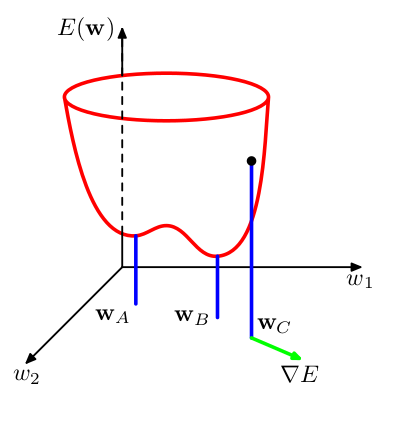
\includegraphics[width=0.55\textwidth]{img/gradsup}
                \caption{Visualización de la función de error $E(\mathbf{w})$ como una superficie. El punto $\mathbf{w}_A$ es un mínimo local y el punto $\mathbf{w}_B$ es el mínimo global. Fuente: \cite{Bishop2006} }
                \label{fig:gradsup}
            \end{figure}

            La actualización de los parámetros dados los gradientes de la red se puede realizar de distintas formas, pero una 
            de las más comunes es el algoritmo llamado \textit{Descenso de gradiente}, donde, de forma iterativa, se 
            va actualizando los pesos restando una medida del gradiente de la siguiente manera:

            Dicho de otro modo, en el descenso de gradiente, se avanza un pequeño paso en la dirección opuesta al gradiente 
            para avanzar hacia el mínimo:

            \begin{equation}
                \mathbf{w}^{(\tau + 1)} = \mathbf{w}^{(\tau)} - \alpha \nabla E(\mathbf{w}^{(\tau)})
            \end{equation}

            donde el parametro $\alpha > 0$ se conoce como la razón de aprendizaje o \textit{learning rate}. Después de 
            cada actualización, el gradiente es recalculado para poder encontrar los nuevos pesos y el proceso se repite 
            hasta encontrar el punto donde $\nabla E = 0$, lo que quiere decir que se ha llegado al mínimo. Usualmente, por 
            la naturaleza de la superficie de la función de error y diversos errores en el cálculo en una computadora, el número 
            de iteraciones se limita en base a cierto parámetro de rendimiento.

            Tradicionalmente, el algoritmo de descenso de gradiente se evalúa sobre todo el conjunto de datos de entrenamiento, 
            este tipo de descenso de gradiente es llamado \textit{batch gradient descent}, una \textit{pasada} por todo el conjunto 
            de entrenamiento se denomina usualmente una \textit{época}. La principal desventaja es que la 
            actualización de los pesos de la red neuronal solamente se actualiza una sola vez en cáda época; esto representa una 
            dificultad en tiempo de procesamiento y memoria cuando se procesan conjuntos de datos muy grandes. Se han desarrollado 
            versiones alternativas al \textit{batch gradient descent} que mejoran su desempeño y son más tratables con 
            conjuntos de datos muy grandes:

            \begin{itemize}
                \item \textbf{\textit{Stochastic Gradient Descent.}} Refiere a que la actualización de los pesos en cada muestra procesada, es decir, que los pesos se actualizan $n$ veces en una época.
                \item \textbf{\textit{Mini-batch Gradient Descent.}} Es una mezcla del descenso de gradiente tradicional y el descenso de gradiente estocástico, en este caso, las muestras se alimentan al algoritmo en \textit{mini-batches} o muestras de tamaño pequeño.
            \end{itemize}
        
            \paragraph{Adam}
            Adam, abreviación de \textit{Adaptive Moment Estimation}, es un algoritmo de optimización alternativo al descenso de 
            gradiente que utiliza promedios tanto de los gradientes como los momentos de segundo orden de los gradientes \cite{kingma2014adam}. Dados 
            los parámetros $\mathbf{w}^{(\tau)}$ y la función de error $E^{(\tau)}$, la actualización de parámetros de acuerdo 
            a Adam se da mediante las siguientes expresiones:

            \begin{align}
                m_w^{(\tau + 1)} &= \beta_1 m_w^{(\tau)} + (1 - \beta_1) \nabla_w E^{(\tau)} \nonumber \\
                v_w^{(\tau + 1)} &= \beta_2 m_w^{(\tau)} + (1 - \beta_2) (\nabla_w E^{(\tau)})^2 \nonumber \\
                \hat{m}_w &= \frac{m_w^{(\tau + 1)}}{1 - (\beta_1)^{(\tau + 1)} } \nonumber \\
                \hat{v}_w &= \frac{v_w^{(\tau + 1)}}{1 - (\beta_2)^{(\tau + 1)} } \nonumber \\
                w^{(\tau + 1)} &= w^{(\tau)} - \alpha \frac{\hat{m}_w}{\sqrt{\hat{v}_w} + \epsilon} \label{eq:adam}
            \end{align}

            Donde $m_w$ representa a los momentos de primer orden y $v_w$ representa a los momentos de segundo orden. Adam 
            tiene los siguientes hiperparámetros:

            \begin{itemize}
                \item $\alpha$ es la razón de aprendizaje, análogo al caso del descenso de gradiente tradicional.
                \item $\beta_1$ es la razón de decaimiento exponencial para el estimado de los momentos de primer orden.
                \item $\beta_2$ es la razón de decaimiento exponencial para el estimado de los momentos de segundo orden.
                \item $\epsilon$ es un escalar pequeño usado para prevenir una posible división entre cero.
            \end{itemize}

            La introducción de los estimados de los momentos de primer y segundo orden de los gradientes permiten que 
            se tome en cuenta el \textit{ímpetu} con el que los gradientes cambian en el proceso de entrenamiento lo cual 
            evita que pueda sobrepasar el mínimo y garantiza su convergencia a mayor velocidad que la de una actualización 
            con un descenso de gradiente tradicional.
            

        \subsubsection{Funciones de activación}
        Se ha estudiado con mucho detalle la naturaleza de la función de activación $f()$, introducida en la 
        Ecuación(\ref{eq:modelobase}), analizando fundamentalmente dos aspectos: su contribución a la generación 
        de representaciones internas en las capas ocultas de la red neuronal, así como también su comportamiento 
        de sus gradientes con relación a la etapa de aprendizaje, tal como se ha visto en la Sección(\ref{sec:gradientes}), 
        donde se ha establecido claramente que el papel de la función de activación y sus gradientes es fundamental para 
        el proceso de retropropagación y ajuste de los pesos de la red. Una guía con algunos criterios puede 
        encontrarse en \cite{mhaskar1994choose}, de donde se rescatan los siguientes aspectos a la hora de escoger una 
        función de activación:
        \begin{itemize}
            \item Que modele de forma no lineal la naturaleza de una representación interna fácil de interpretar.
            \item Que sea derivable en todo el rango de trabajo.
        \end{itemize}

        Tomando en cuenta lo anterior, se han generado diversas tendencias en la aplicación de funciones de activación y a 
        continuación se analizarán las más relevantes para este proyecto.
            \paragraph{Función sigmoide}\label{sec:sigmoide}
            Esta función ha sido introducida en la Ecuación(\ref{eq:sigmoide}) y representa, históricamente, la función 
            más utilizada en las primeras redes neuronales artificiales porque modela de manera aproximada, una respuesta 
            característica de las neuronas del cerebro \cite{narayan1997generalized}, pero sobre todo, porque posee las dos características mencionadas 
            anteriormente: naturaleza no lineal y diferenciable. Otra característica llamativa, es que se puede interpretar 
            a la salida como una función de probabilidad, pues sus valores van desde $0$ a $1$, como se puede apreciar 
            en la Figura(\ref{fig:sigmoide}). Usualmente se incluye un parámetro adicional para controlar el \textit{radio de activación}
            que hace que la función responda con más o menos sensibilidad a su entrada.

            \begin{figure}[!h] 
                \centering
                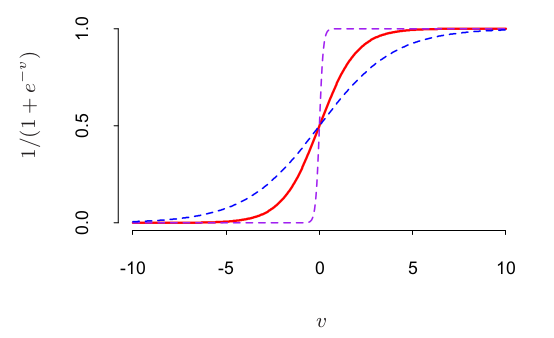
\includegraphics[width=0.75\textwidth]{img/sigmoide}
                \caption{Gráfico de la función sigmoide $\sigma(v) = 1 / (1 + e^{(-v)})$ (curva roja), y dos variaciones con un radio de activación de la forma $\sigma(sv)$ con valores $s=1/2$ (curva azul) y $s=10$ (curva púrpura) . Fuente: \cite{Goodfellow-et-al-2016} }
                \label{fig:sigmoide}
            \end{figure}
            
            Pese a las características anteriormente mencionadas, la función sigmoide tiene una gran desventaja: el llamado 
            \textit{desvanecimiendo de gradientes} \cite{hochreiter1998vanishing}. Este fenómeno ocurre cuando la activación 
            de una capa oculta tiene valores muy altos o muy negativos, se puede apreciar en la Figura(\ref{fig:sigmoide}), que 
            para estos valores, la derivada tiene un valor muy pequeño, aproximándose a cero mientras más grandes sean los valores.
            Este fenómeno ocasiona que, mientras se realiza la retropropagación de gradientes, dado que el gradiente tiene un valor 
            muy bajo, el ajuste en los pesos sea mínimo, deteniendo así el aprendizaje de la neurona en la que ocurre el fenómeno.

            Esta dificultad se presenta especialmente cuando la red neuronal se compone de varias capas ocultas y 
            ha motivado el desarrollo de nuevas funciones de activación que no presenten esta limitación y puedan 
            mantener valores de gradientes adecuados durante el entrenamiento.
            
            Cabe resaltar que, pese a las dificultades con la propagación de los gradientes de la función sigmoide, ésta se suele 
            utilizar bastante en la capa de salida, cuando se trata de clasificación binaria, ya que representa de manera adecuada
            la noción de probabilidad, lo cual es deseable en este tipo de modelos.

            \paragraph{Función tangente hiperbólica} \label{sec:tanh}
            La función tangente hiperbólica o $tanh()$ se define mediante la siguiente expresión:

            \begin{equation}\label{eq:tanh}
                tanh(x) = \frac{e^x - e^{-x}}{e^x + e^{-x}}
            \end{equation}

            Esta función también cumple con los requisitos de no linealidad y de ser derivable, pero en este caso, el rango de 
            salida de la función $tanh()$ es desde $-1$ a $1$. Considerando el concepto de función de probabilidad que ofrece 
            la salida de la función sigmoide, la función tangente hiperbólica introduce el concepto de aceptación o negación 
            de una premisa, donde una premisa aceptada se acerca a 1 y una premisa rechazada se acerca a -1, el valor de 0, 
            indica indecisión. La función $tanh()$ se ha usado junto a su par sigmoide ampliamente en los inicios de las redes 
            neuronales para las activaciones de las capas ocultas, pero, tal como se puede observar en la Figura(\ref{fig:tanh}), 
            presenta la misma desventaja del desvanecimiendo de gradientes, dado que para valores muy grandes, la derivada se 
            aproxima a cero.

            \begin{figure}[!h] 
                \centering
                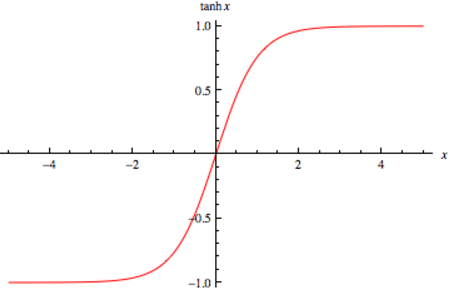
\includegraphics[width=0.75\textwidth]{img/tanh}
                \caption{Gráfico de la función tangente hiperbólica $tanh(x) = \frac{e^x - e^{-x}}{e^x + e^{-x}}$. Fuente: \cite{wang_2016} }
                \label{fig:tanh}
            \end{figure}

            En la actualidad, para implementaciones de redes neuronales profundas, el uso de las funciones sigmoide y tangente 
            hiperbólica en las capas ocultas está ampliamente desaconsejado por los problemas anteriormente planteados. En su 
            lugar se ha generado nuevos tipos de funciones de activación que presentan características bastante favorables 
            para el aprendizaje y ajuste de pesos basados en gradientes.

            \paragraph{Unidad Lineal Rectificada - ReLU}
            Introducida por primera vez en el año 2010 por Nair y Hinton, las Unidades Lineales Rectificadas o ReLU, se 
            propusieron para mejorar el rendimiento de un tipo especial de red neuronal: las máquinas restringidas de Boltzman 
            (RMB, por sus siglas en inglés) \cite{nair2010rectified}, pero pronto, ganarían gran popularidad también en las 
            redes neuronales feedforward y en redes neuronales convolucionales como se puede apreciar en \cite{krizhevsky2012imagenet}.
            
            La función ReLU se define de la siguiente manera:

            \begin{equation}\label{eq:relu}
                g(x) = max\{0,x\}
            \end{equation}

            Tal como se puede apreciar, la característica más importante de la función ReLU es su simplicidad pues es muy 
            similar a una función identidad, la diferencia es que ReLU toma el valor de cero para todos los valores de $x$ que 
            sean negativos. Esto resuelve el problema del desvanecimiendo de gradientes pues garantiza que el gradiente 
            tenga un valor razonable si la entrada está activa y además sea consistente.

            \begin{figure}[!h] 
                \centering
                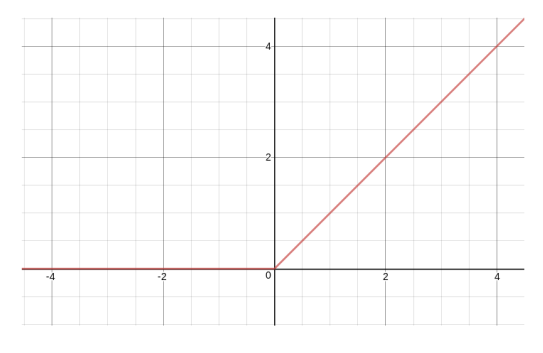
\includegraphics[width=0.75\textwidth]{img/relu}
                \caption{Gráfico de la ReLU. Fuente: \cite{wang_2016} }
                \label{fig:relu}
            \end{figure}

            Sin embargo, dado que la función ReLU tiene una gradiente nula para valores negativos es de vital importancia 
            que se garantice la existencia de gradientes positivos, aunque sea pequeños durante la inicialización y las capas 
            previas.

        \subsubsection{Diseño de Arquitectura e hiperparámetros de una red neuronal}
        Como se ha podido ver en las secciones anteriores, la característica más importante de una red neuronal es que es capaz
        de generar representaciones internas a partir de los datos y la retropropagación de los gradientes, lo que ha finalizado la era 
        de la ``ingeniería de características'' donde se necesitaba conocimiento experto para elegir las representaciones adecuadas y cómo calcularlas, sin embargo, esto 
        ha llevado a que el diseño de las redes se enfoque en otros aspectos como la arquitectura y otros parámetros externos 
        que definen el modelo de la red. Por arquitectura de la red, se entiende a la estructura general de la red neuronal, 
        el número de capas, el número de unidades o neuronas por cada capa y cómo las unidades y capas se conectan entre sí.

        La gran parte de las redes neuronales estan organizadas en grupos de unidades llamadas capas, asimismo, las capas se 
        ordenan de manera encadenada siendo cada capa una función de la capa que la precede, esto se ha establecido para una red de 
        dos capas en la Ecuación(\ref{eq:reddoscapas}) en su forma general, pero, se puede expresar el modelo de forma vectorial
        de la siguiente manera:

        \begin{align}
            \mathbf{h}^{(1)} &= g^{(1)} \left( \mathbf{W}^{(1)T}\mathbf{x} + \mathbf{b}^{(1)} \right) \\
            \mathbf{h}^{(2)} &= g^{(2)} \left( \mathbf{W}^{(2)T}\mathbf{h}^{(1)} + \mathbf{b}^{(2)} \right)
        \end{align}

        En términos de redesn neuronales, la cantidad de unidades en cada capa se denomina el ancho o \textit{width} 
        y la cantidad de capas se denomina profundidad o \textit{depth}.

            \paragraph{Hiperparámetros}
            Tanto la profundidad como el ancho de la red, son parámetros que se deben escoger en base a ciertos criterios, 
            éstos parámetros son externos a los parámetros o pesos $\mathbf{W}$ de la red neuronal, por lo que se demoninan
            hiperparámetros. Aparte del ancho y profundidad, en el diseño de una red neuronal se consideran las siguientes 
            variables:

            \begin{itemize}
                \item Razón de aprendizaje $\alpha$.
                \item Funciones de activación.
                \item Tamaño del \textit{mini-batch}.
                \item Número de épocas de entrenamiento.
                \item Algoritmo optimizador (Ejemplo: Descenso de gradiente).
                \item Función de costo.
            \end{itemize}

            Los hiperparámetros deberán ser escogidos de manera cuidadosa, pero debido a la gran complejidad y poca predictibilidad
            del comportamiento de una red neuronal profunda normalmente se eligen en conjunto con un proceso de prueba y error, 
            analizando las curvas de aprendizaje y rendimiento en conjuntos de datos de validación y prueba.

    \subsection{Redes Neuronales Convolucionales}
    Las redes neuronales convolucionales son un tipo especializado de red neuronal que 
    sirven para procesar datos de tipo "grilla" \cite{Goodfellow-et-al-2016}. Algunos ejemplos 
    de datos de tipo grilla que se pueden mencionar son los siguientes:
    \begin{itemize}
        \item \textbf{Series de tiempo.} Grilla de una dimensión tomados en intervalos regulares de tiempo.
        \item \textbf{Imágenes digitales.} Grilla de pixeles de dos o más dimensiones (Escala de grises, RGB).
    \end{itemize}

    Las también llamadas redes convolucionales, han demostrado un éxito impresionante en diversas 
    aplicaciones prácticas especialmente en el campo de la visión por computador y el procesamiento de texto y lenguaje natural. 
    El término ``red neuronal convolucional'' proviene del hecho de que en este tipo 
    de redes neuronales se utiliza una operación matemática llamada \textbf{convolución}, siendo la convolución 
    una operación lineal especializada para procesar datos de tipo grilla.

    En los párrafos posteriores, se procede a describir la operación de convolución en el contexto de 
    redes neuronales, pues, no siempre la definición de la misma corresponde con el concepto de convolución
    usado en distintos campos de la ciencia y la ingeniería.

        \subsection{Operación de convolución}
        En su forma más general, la convolución es una operación entre dos funciones reales y su definición se puede introducir
        usando el concepto de un promedio ponderado. Sea una función $x(t)$ dependiente del tiempo, 
        tanto $x$ como $t$ son números reales; en este caso, la función $x$ puede entenderse como una serie de medidas
        en un instante de tiempo $t$. Considérese una segunda función de ponderación $w(\tau)$ donde $\tau$ es la antiguedad 
        de una medida. Si se aplica la función de ponderación en cada instante de tiempo, se puede obtener una nueva función 
        definida por:
        \begin{equation}
            s(t) = \int x(\tau)w(t - \tau) d\tau
        \end{equation} 
        Esta operación es llamada la \textit{operación de convolución} y es denotada tradicionalmente con un asterisco:
        \begin{equation}
            s(t) = (x\ast w)(t)
        \end{equation}
        En el ejemplo de la ponderación, $w$ debe ser una función de densidad de probabilidad válida, o la salida no podrá
        ser considerada como un promedio ponderado. Además, $w$ también debe ser $0$ para cualquier $t<0$, esta última 
        característica se denomina comunmente como el principio de ``causalidad''. En general, la convolución está 
        definida para cualquier función en la cual la integral anteriormente declarada esté definida y puede ser 
        usada para otros propósitos aparte de promedios ponderados.

        Hablando en términos de una red neuronal convolucional, el primer argumento (en el ejemplo, la función $x$) 
        es comunmente referido como la \textbf{entrada}, y el segundo argumento ($w$, en el ejemplo) es referido 
        como el \textbf{kernel}. La salida, a su vez, es normalmente referida como el \textbf{mapa de características}.
        
        Por su parte, cuando se trata de señales digitales, como los datos en una computadora, el tiempo tiene una 
        naturaleza discreta, es decir, que los datos estarán disponibles en intervalos regulares de tiempo. En este 
        caso, el índice de tiempo $t$ puede tomar solamente valores enteros y, entonces, es válido asumir 
        que tanto $x$ como $w$ estan definidos solamente para valores enteros de $t$. De este modo, 
        se puede definir la convolución discreta:
        \begin{equation}
            s(t) = (x \ast w)(t) = \sum_{\tau=-\infty}^{\infty}x(\tau)w(t-\tau)
        \end{equation}

        En el contexto de las aplicaciones de aprendizaje automático o, más específicamente, aprendizaje profundo,
        la entrada es usualmente un arreglo multidimensional de datos, y el kernel es usualmente un arreglo 
        multidimensional de parámetros que se adaptan en el proceso de aprendizaje. 

        \subsubsection{Procesamiento de imágenes con redes neuronales convolucionales}
        La operación de convolución se usa frecuentemente sobre datos con más de una dimensión. Las imágenes digitales 
        son un perfecto ejemplo de un arreglo multidimensional de datos. Una imagen digital se representa mediante una
        matriz con filas y columnas, donde cada elemento se denomina pixel y contiene información acerca de la intensidad
        o luminancia, para una imagen en escala de grises o el nivel de color para distintos canales en una imagen a color.
        Si se toma el ejemplo de la imagen en escala de grises, se tiene una entrada o imagen bidimensional $I$ con un
        kernel bidimensional correspondiente $K$:

        \begin{equation} \label{eq:conv2d}
            S(i,j)=(I\ast K)(i,j) = \sum_{m} \sum_{n} I(m,n)K(i-m,j-n)
        \end{equation}

        Dado que la convolución es conmutativa, se puede reescribir la ecuación \ref{eq:conv2d} como:

        \begin{equation}
            S(i,j)=(K\ast I)(i,j) = \sum_{m} \sum_{n} I(i-m,j-n)K(m,n)
        \end{equation}

        Frecuentemente, la última fórmula es la más utilizada en librerías de aprendizaje profundo 
        por su sencillez en la implementación en un sistema computacional, esto, dado que existe menos 
        variación en el rango de valores válidos de $m$ y $n$. En la Figura(\ref{fig:convolucion}), se 
        puede apreciar una visualización de la operación de convolución aplicada a una imagen. 


        \begin{figure}[!h] 
            \centering
            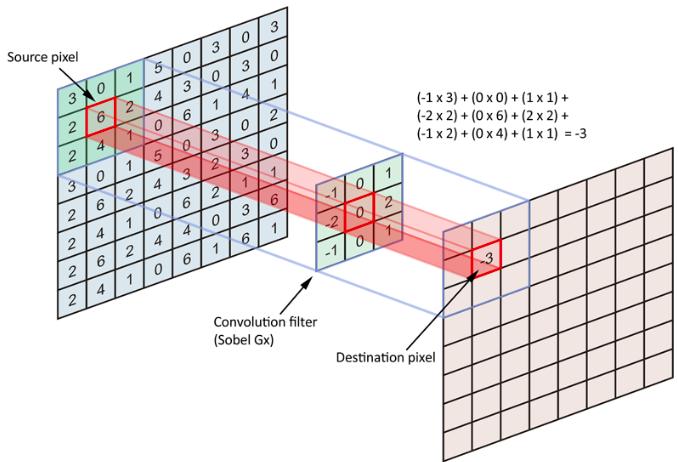
\includegraphics[width=0.75\textwidth]{img/convolucion}
            \caption{Visualización de la operación de convolución sobre una imagen digital. Fuente: \cite{cornelisse_2018} }
            \label{fig:convolucion}
        \end{figure}


        

        \subsubsection{Aprendizaje de representaciones internas}
        Una de las preguntas clave en la visión por computador es el cómo generar una buena y significativa
        representación interna de una imagen, dado que la mayor parte de la imagen corresponde con pixeles que no 
        aportan mucha información relevante a la tarea asignada. Por ejemplo, si se quisiera detectar 
        un rostro dentro de una imagen, normalmente se suele encontrar una representación que ayude a aislar solamente 
        las porciones de la imagen que pueden contener el rostro, tales como la búsqueda de contornos, bordes y 
        características típicas de un rostro. Antes de la aparición de las redes convolucionales, estas representaciones 
        se hallaban de manera manual y gracias al conocimiento de expertos en el área del procesamiento de imágenes. 
        La definición de características y mapas de características era comunmente conocida como la 
        \textit{ingeniería de características}, en la cual los expertos creaban descriptores para tareas específicas con 
        una gran inversión de tiempo en la sintonización fina de los mismos. 

        % TODO: poner el ejemplo de viola jones 

        En contraste con el anterior enfoque, las redes convolucionales generan sus propias representaciones internas
        de manera automática gracias al aprendizaje de los parámetros de cada uno de los kernels que componen las distintas 
        capas de la red neuronal. En principio, las redes convolucionales se inspiraron en el trabajo de Hubel y Wiesel 
        sobre la corteza visual primaria de un gato\cite{lecun2010convolutional}. En dicho trabajo, se logró identificar células simples que respondían
        de manera sobresaliente a distintas orientaciones con campos receptivos locales. Éstas células receptivas simples 
        se pueden corresponder con los kernels de convolución usados en las redes convolucionales por la sencillez y la 
        localidad de su campo de receptividad.

        Posteriormente, las redes convolucionales ganaron una gran popularidad debido a su rendimiento en tareas de 
        clasificación de imágenes y detección y reconocimiento de objetos en imágenes. El primer hito de su capacidad 
        para procesar imágenes de manera efectiva fue en concurso de clasificación de imágenes de ImageNet, donde 
        el equipo de Geoffrey Hinton logró sobrepasar el mejor resultado en precisión de clasificación por un gran márgen 
        usando una arquitectura de red convolucional \cite{krizhevsky2012imagenet}. En este trabajo, se pudo apreciar con 
        gran detalle las ventajas del enfoque del aprendizaje de representaciones internas en una red convolucional.

        \begin{figure}[!h] 
            \centering
            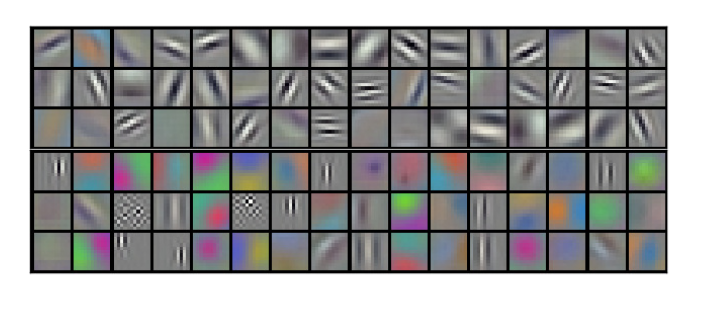
\includegraphics[width=0.75\textwidth]{img/fmap_imagenet}
            \caption{Kernels convolucionales de tamaño $11 \times 11 \times 3$ en la primera capa convolucional. Fuente: \cite{krizhevsky2012imagenet} }
            \label{fig:fmap_imagenet}
        \end{figure}
            
        Tal como se puede apreciar en la Figura(\ref{fig:fmap_imagenet}), en la primera capa convolucional, 
        los kernels de convolución corresponden con representaciones básicas en una imagen como la búsqueda de 
        bordes en distintas orientaciones, esto va acorde a lo establecido anteriormente en el modelo de 
        la corteza visual de un gato. Puede decirse entonces que las redes convolucionales emulan, en cierto modo, 
        al proceso biológico de visión en animales.

 
    \subsection{Sistemas de Aprendizaje Fin a Fin}
    Los sistemas de aprendizaje fin a fin refieren a sistemas complejos que se conciben, modelan y entrenan 
    como un conjunto para resolver cierto problema en vez de tratarse de forma separada por módulos. En términos
    de redes neuronales, los sistemas de aprendizaje fin a fin refieren a redes neuronales complejas, compuestas 
    por distintos componetes y tipos de unidades que usualmente tratan un problema de aprendizaje en su totalidad.
    
    En contraste con el desarrollo de los sistemas de aprendizaje tradicionales, tal como se pudo apreciar 
    en la Sección(\ref{sec:problema}) donde cada etapa del proceso debía ser cuidadosamente diseñada y evaluada por alguien 
    con la experiencia suficiente en el área, los sistemas fin a fin, dejan la responsabilidad de encontrar 
    las representaciones internas adecuadas al proceso de entrenamiento de la red neuronal en sí. Las representaciones
    adecuadas son generadas a partir del proceso de aprendizaje y ajuste de pesos en las distintas capas ocultas de la red 
    neuronal. Usualmente, las redes neuronales para aplicaciones de aprendizaje fin a fin se componen de varias etapas 
    de distinta naturaleza, de acuerdo al problema que se intenta resolver. 

    Los sistemas de aprendizaje fin a fin han demostrado ser una alternativa bastante llamativa debido a que presentan 
    las siguientes ventajas:

    \begin{itemize}
        \item \textbf{Diseño simplificado.} El diseño de un 
        sistema fin a fin es mucho menos demandante en cuestión de tiempo y conocimiento experto, la extracción de características
        no necesita ser una etapa elaborada por un experto pues se generará automáticamente.
        \item \textbf{Entrenamiento centralizado.} Dado que se trata de una sola red neuronal profunda que se incorporará en 
        el flujo de trabajo, el entrenamiento de la misma se realiza de forma única para todo el sistema.
        \item \textbf{Flexibilidad.} Debido a que el proceso de diseño solamente introduce criterios generales para la tarea 
        deseada, los sistemas fin a fin pueden ser fácilmente adaptados para realizar otras tareas en el futuro. Las iteraciones 
        en el diseño y entrenamiento no requieren de mucho tiempo ni esfuerzo. 
        \item \textbf{Modularidad.} La naturaleza de las representaciones internas generadas en las redes neuronales profundas 
        permite que las mismas se puedan reutilizar en otras tareas o arquitecturas.
    \end{itemize}

    Gracias a las ventajas anteriormente descritas, los avances en el desarrollo de sistemas 
    fin a fin han tenido particular éxito en las siguientes áreas:

    \begin{itemize}
        \item Reconocimiento de voz \cite{graves2014towards}.
        \item Control de brazos robóticos \cite{levine2016end}.
        \item Conduccion autónoma. \cite{bojarski2016end}.
    \end{itemize}

    En el presente proyecto, se utilizarán los conceptos de aprendizaje profundo, redes convolucionales y aprendizaje 
    fin a fin para diseñar un sistema de conducción autónoma.

\section{Robots móviles y locomoción con ruedas}
Un robot móvil es una máquina electromecánica con ciertos niveles de autonomía definida que son capaces de moverse 
y navegar por un entorno. Las ruedas aprovechan la fricción y el contacto con el suelo para hacer que el robot pueda moverse. 
Si se considera un vehículo ideal, donde las ruedas no se deslizan hacia los costados y mantienen contacto con el suelo en 
todo momento, para que exista un movimiento debe existir un punto alrededor del cual cada rueda sigue una trayectoria circular.
Este punto es conocido como el Centro Instantáneo de Rotación o Curvatura (ICC). En la práctica, el ICC se puede identificar de manera 
sencilla porque es el punto que yace en una linea coincidente con el eje de rotación de cada rueda. El ICC define la curvatura 
de la trayectoria que sigue el robot en cada momento. En la Figura(\ref{fig:icc}), se puede apreciar una configuración compatible 
con el movimiento sin deslizamiento de las ruedas y una configuración incompatible.

\begin{figure}[!h] 
    \centering
    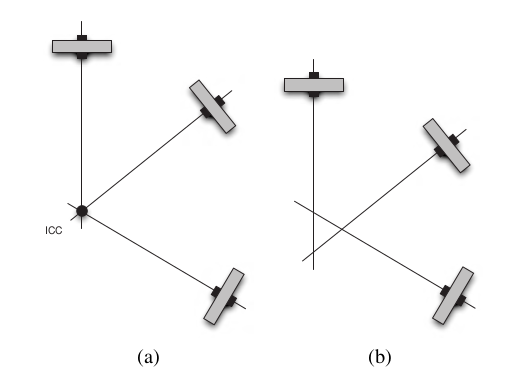
\includegraphics[width=0.75\textwidth]{img/icc}
    \caption{Centro instantáneo de curvatura o ICC. (a) Arreglo compatible con el movimiento, (b) arreglo incompatible con el movimiento. Fuente: \cite{krizhevsky2012imagenet} }
    \label{fig:icc}
\end{figure}


La existencia del ICC es una condición necesaria pero no suficiente para el movimiento de un robot con ruedas, también las 
velocidades de cada rueda deben ser consistentes con la rotación rígida del vehículo en su conjunto. Un robot localizado en 
un plano tiene tres grados de libertad: una posición $(x,y)$ y una orientación $\theta$. Este conjunto de parámetros $(x,y,\theta)$ 
es comúnmente denominado la pose del robot en el plano.

Los robots móviles usualmente no poseen un control absoluto sobre los tres parámetros de su pose y deben realizar diversas 
maniobras para poder alcanzar una pose en particular. Estas restricciones en el control de su movimiento se conocen como 
restricciones no holonómicas. 

    \subsection{Modelo de locomoción de Ackerman}
    Es el tipo de locomoción encontrada en la mayoría de los automóviles domésticos. En este modelo, las ruedas frontales estan 
    direccionadas y pueden rotar distintos ángulos de tal manera que sus ejes de rotación se intersectan en el ICC. La rueda 
    direccionada interna debe rotar un ángulo un poco mayor que la externa para que la condición se cumpla Figura(\ref{fig:ackerman}).


    \begin{figure}[!h] 
        \centering
        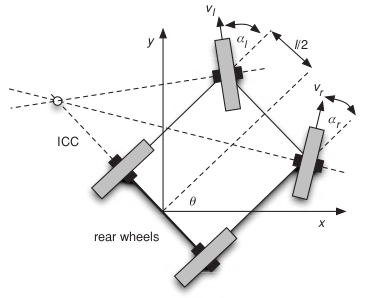
\includegraphics[width=0.75\textwidth]{img/ackerman}
        \caption{Modelo cinemático de Ackerman. Fuente: \cite{GregoryMcGillUniversity2010} }
        \label{fig:ackerman}
    \end{figure}

    La locomoción de Ackerman es la preferida en vehículos de gran tamaño, los cuales están diseñados para operar en carreteras
    existentes y soportar una carga considerable. Normalmente, el tamaño del vehículo permite incorporar una gran cantidad 
    de sensores y sistemas de control. 
        \subsubsection{Cinemática directa}
        El vehículo rota alrededor de un punto que yace en la linea que pasa por el eje trasero una distancia $R$ del centro 
        del vehículo donde

        \begin{equation*}
            R - l/2 = d \tan{(\pi / 2 - \alpha_l)}
        \end{equation*}

        Para que las ruedas puedan rodar la segunda rueda de dirección debe ser rotada un ángulo $\alpha_r$, donde 

        \begin{equation*}
            R + l/2 = d \tan{(\pi / 2 - \alpha_r)}
        \end{equation*}

        En general, las cuatro ruedas viajan por el suelo a velocidades diferentes y al especificar la velocudad de una sola rueda
        se puede obtener las velocidades de las restantes. El modelo de locomoción de Ackerman es muy sofisticado y ha sido 
        estudiado ampliamente. Para los objetivos del presente proyecto, se puede simplificar el modelo sin perder ninguna 
        propiedad importante.

    \subsection{Modelo de la bicicleta o triciclo} \label{sec:triciclo}
    Los modelos de la bicicleta y el triciclo tienen modelos cinemáticos muy similares. Un triciclo típico tiene tres ruedas: 
    dos ruedas de tracción traseras y una rueda de dirección delantera. El movimiento del robot es controlado por la dirección 
    $\alpha$ y la velocidad $v$.
    \begin{figure}[!h] 
        \centering
        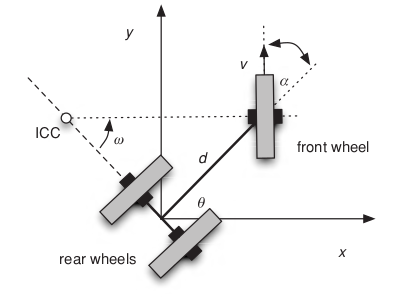
\includegraphics[width=0.75\textwidth]{img/triciclo}
        \caption{Modelo cinemático del triciclo. Fuente: \cite{GregoryMcGillUniversity2010} }
        \label{fig:triciclo}
    \end{figure}    

        \subsubsection{Cinemática directa}
        Si la rueda de dirección se orienta en un ángulo $\alpha$ de la dirección hacia adelante, el triciclo rotará con una 
        velocidad angular $\omega$ con respecto al punto que yace a una distancia $R$ de la línea perpendicular que pasa 
        por el eje trasero donde $R$ y $\omega$ están dados por las siguientes expresiones:

        \begin{align}
            R       &= d \tan(\frac{\pi}{2} - \alpha) \\
            \omega  &= \sqrt{\frac{v}{d^2 + R^2}}
        \end{align}

        donde $d$ es la distancia desde la rueda frontal al eje trasero, como se observa en la Figura(\ref{fig:triciclo}).

    
    En el presente proyecto, se considerará el uso del modelo del triciclo definido en la Sección(\ref{sec:triciclo}) 
    por razones de simplicidad.


\chapter{Ingeniería del proyecto}\label{ch:ingenieria}
\section{Arquitectura del sistema}\label{sec:arquitectura}
En la presente sección se procede a detallar la arquitectura del sistema de forma general analizando cada uno de 
los subsistemas, sus funcionalidades, componentes y características. Posteriormente se detallarán los detalles técnicos
y de implementación de cada subsistema. Para comenzar, es necesario describir la visión general del sistema, la finalidad 
y alcance del mismo.

    \subsection{Visión general}
    Tal como se ha establecido en el Capítulo(\ref{ch:introduccion}), el objetivo del presente proyecto es el de diseñar 
    un sistema de aprendizaje fin a fin para la tarea de conducción autónoma en vehículos domésticos. Este sistema ha sido 
    diseñado con la finalidad de plantear una alternativa para el desarrollo de sistemas de conducción autónoma en especial 
    en el subsistema de inferencia y control autónomo. No obstante, se ha desarrollado un prototipo completamente funcional 
    de un vehículo autónomo que cumple la tarea de seguir una carretera y detenerse cuando un obstáculo se interpone de 
    manera autónoma. 

    Es importante destacar que este proyecto también brinda un conjunto de herramientas de software 
    y hardware de manera que se pueda replicar el mismo de forma fácil y con un presupuesto reducido. Si bien el 
    presente proyecto se centra en el desarrollo 
    del sistema de visión artificial para la generación de comandos de dirección usando una red neuronal convolucional, la 
    naturaleza modular de la arquitectura del mismo permite realizar cambios o mejoras en cada uno de los subsistemas. Estos 
    cambios y mejoras se pueden introducir aprovechando la naturaleza modular de los nodos de ROS y la infraestructura de 
    comunicación presente en el sistema pudiendo agregarse más de un sistema de control en el mismo, como por ejemplo, un 
    sistema de reconocimiento de peatones o señales de tránsito.

    \subsection{Esquema del sistema}

    Se procede a detallar el esquema general del sistema en base a la interacción de tres subsistemas básicos en la Figura(\ref{fig:arquitectura}). 

    \begin{figure}[!h] 
        \centering
        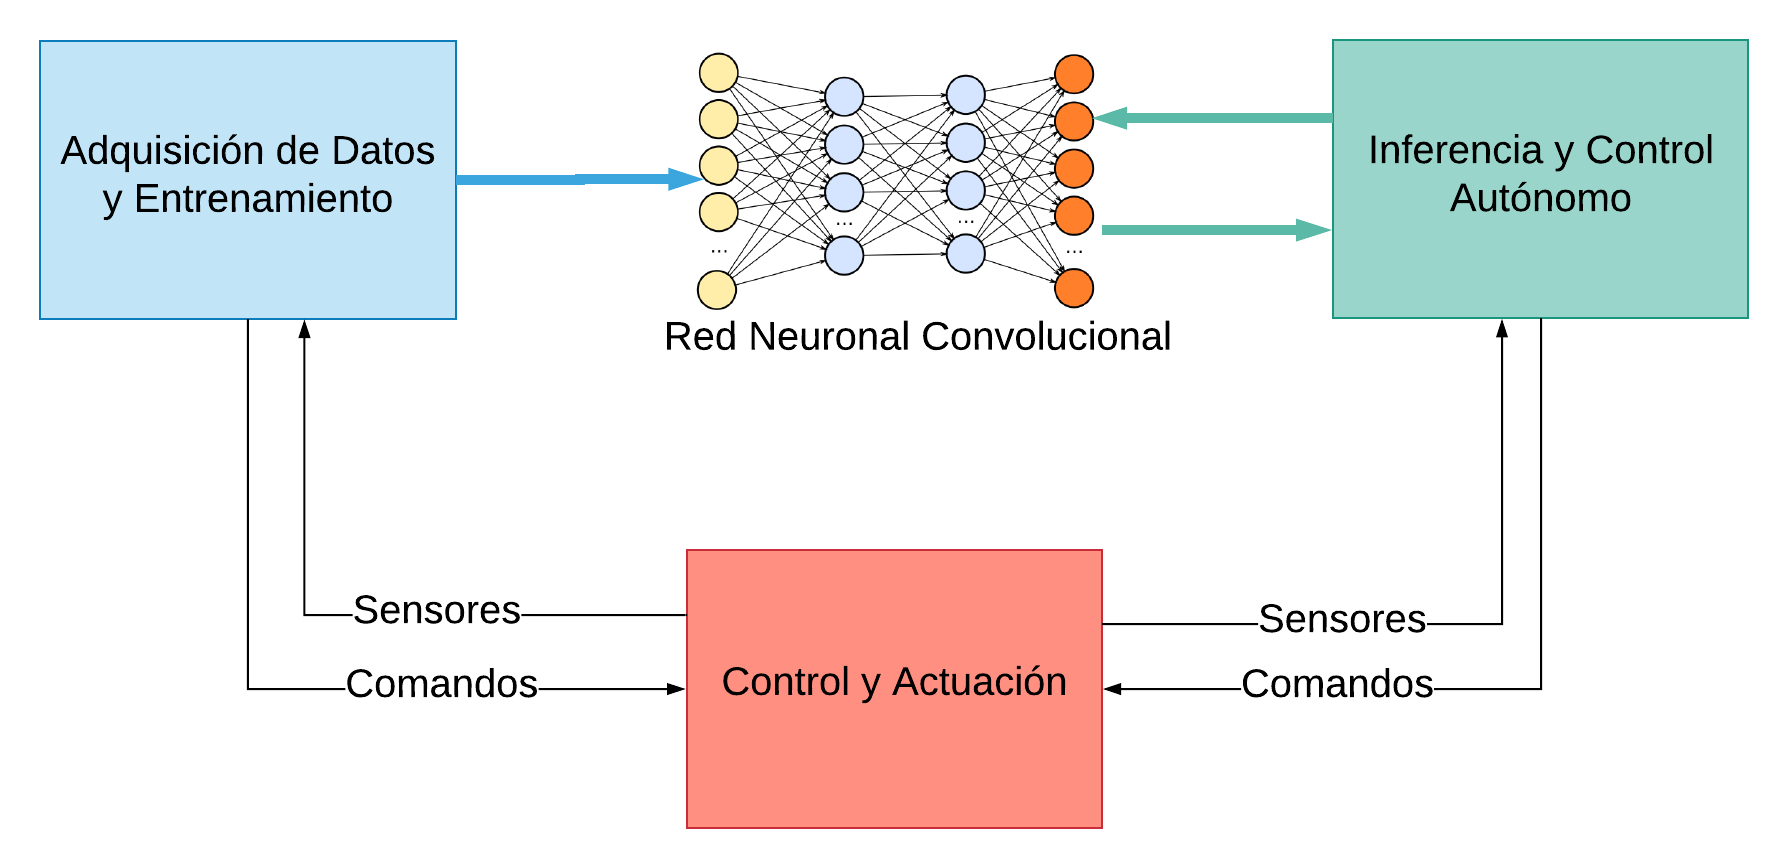
\includegraphics[width=0.85\textwidth]{img/arquitectura}
        \caption[Esquema en diagrama de bloques del sistema]{Esquema en diagrama de bloques del sistema. Fuente: Elaboración propia. }
        \label{fig:arquitectura}
    \end{figure}

    En el esquema, se puede observar la interacción entre los subsistemas que componen el sistema en su conjunto haciendo 
    un énfasis en la comunicación entre el subsistema de control y actuación y los otros dos subsistemas. El sistema de 
    control y actuación representa la plataforma sobre la cual se van a ejecutar los otros dos subsistemas, el de adquisición 
    de datos y entrenamiento en primer lugar, para el entrenamiento de la red neuronal y seguidamente el de inferencia 
    y control autónomo en el que se usará la información generada por el primero para lograr la tarea de conducción autónoma. 
    
    Este esquema es particularmente popular y bien establecido en muchos sistemas de aprendizaje automático en el que se cuenta,
    por un lado, con una forma de obtener y adecuar los datos para el entrenamiento de la red y, por el otro, se tiene una 
    etapa de inferencia o predicción en la cual se valida la eficacia del modelo. En este caso, la planta o el sistema donde 
    se puede validar la eficacia de la red neuronal es el prototipo con el vehículo.

    En las siguientes secciones se detalla la arquitectura de cada subsistema exponiendo sus diagramas de bloques asociados.

    \subsection{Subsistema de control y actuación} \label{sec:esqcontrol}
    El subsistema de control y actuación tiene el objetivo de servir como base física para la implementación de los algoritmos 
    de control. En la Figura(\ref{fig:control_esq}) se puede apreciar sus componentes y la forma en que interactúan entre sí. 
    Este subsistema cuenta con varios módulos funcionales que se encargan del control y actuación del vehículo. Los módulos 
    tienen la tarea de brundar una plataforma para que los algoritmos de control se puedan ejecutar en el vehículo. 

    Este subsistema cuenta con módulos que tienen tres principales responsabilidades.
    
    \begin{itemize}
        \item Ejecutar un control de tiempo real en los actuadores disponibles para la locomoción del vehículo a través de un sistema embebido.
        \item Brindar una plataforma para la adquisición de los datos de los sensores (la cámara y el sensor de proximidad).
        \item Brindar una plataforma de desarrollo para el control autónomo del vehículo mediante ROS (Sección(\ref{sec:ros})).
    \end{itemize}

    \begin{figure}[!h] 
        \centering
        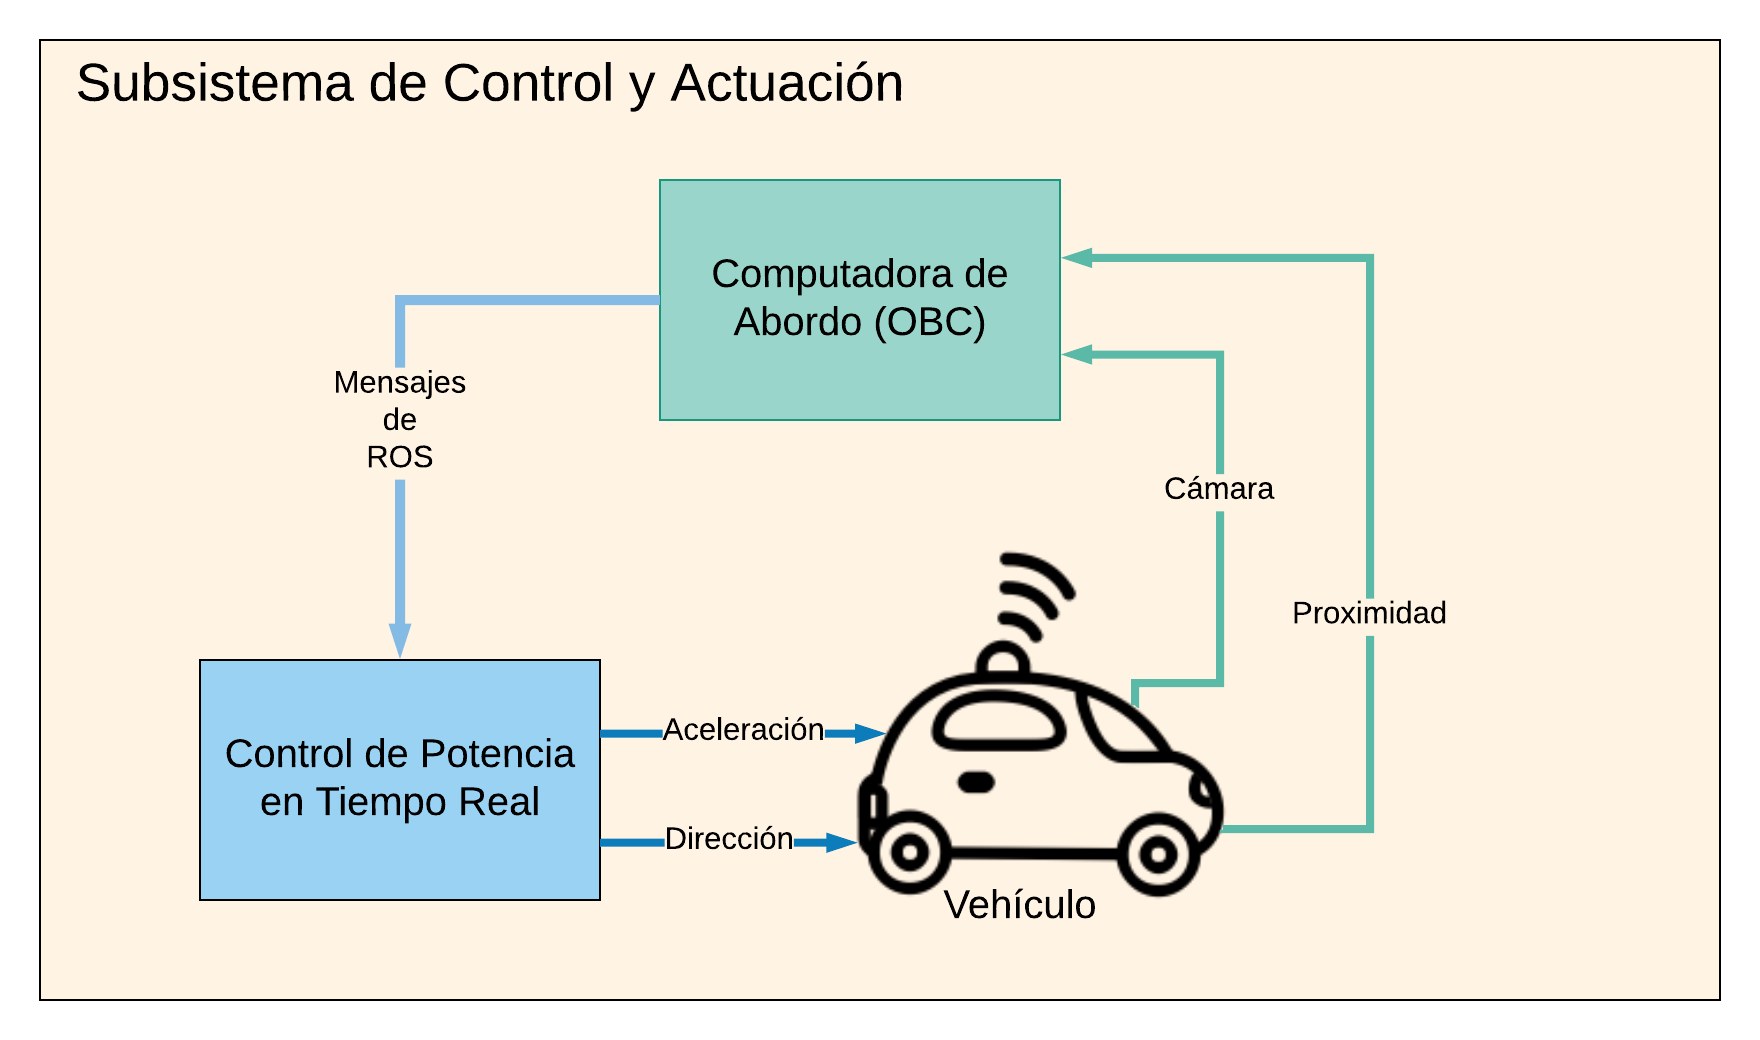
\includegraphics[width=0.85\textwidth]{img/control_esq}
        \caption[Subsistema de control y actuación]{Esquema en diagrama de bloques del Subsistema de control y actuación. Fuente: Elaboración propia. }
        \label{fig:control_esq}
    \end{figure}

    \subsection{Subsistema de adquisición de datos y entrenamiento}\label{sec:esqdaq}
    El subsistema de adquisición de datos y entrenamiento tiene la finalidad de proporcionar las herramientas necesarias para 
    dos tareas fundamentales:
    \begin{itemize}
        \item Generar un conjunto de datos o \textit{dataset} para el entrenamiento y validación de la red neuronal.
        \item Entrenar una red neuronal a partir del conjunto de datos y ciertos parámetros previamente definidos.
    \end{itemize}

    Para tal cometido, este subsistema cuenta con varios módulos que interactúan entre sí y brindan distintas funcionalidades.
    En la Figura(\ref{fig:daq_esq}). Es importante destacar que la naturaleza de los módulos de este subsistema hicieron que 
    los mismos se deban ejecutar en una estación de trabajo remota con características especiales para las tareas necesarias. 
    Esta forma de trabajo se ha adoptado para disminuir el tiempo necesario en la tarea del entrenamiento de la red neuronal 
    la cual es una tarea que demanda mucho poder computacional.

    \begin{figure}[!h] 
        \centering
        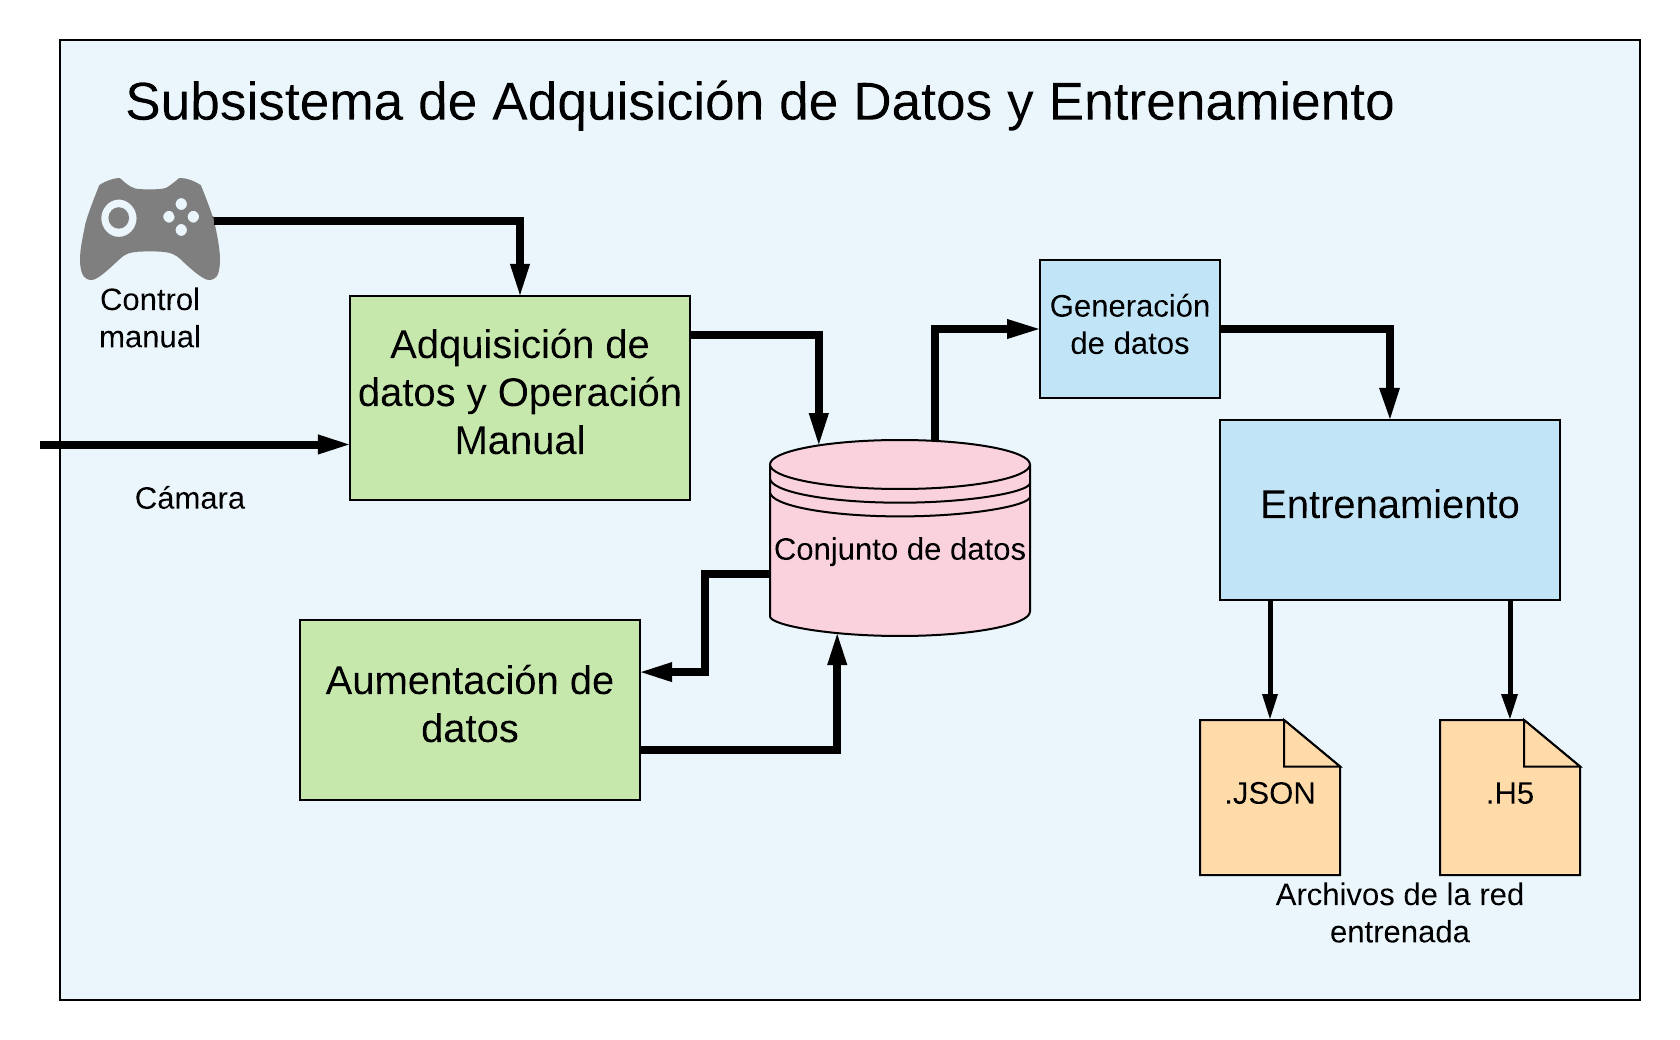
\includegraphics[width=0.85\textwidth]{img/daq_esq}
        \caption[Subsistema de Adquisición de datos y Entrenamiento]{Esquema en diagrama de bloques del Subsistema de Adquisición de datos y Entrenamiento. Fuente: Elaboración propia. }
        \label{fig:daq_esq}
    \end{figure}

    El producto de este subsistema es un conjunto de archivos que representan tanto la arquitectura de la red neuronal como 
    los datos de los pesos obtenidos en el proceso de entrenamiento. Dichos archivos serán utilizados en el subsistema 
    de inferencia y control autónomo.

    \subsection{Subsistema de inferencia y control autónomo}\label{sec:esqinferencia}
    En este subsistema se concentra la mayor complejidad del sistema siendo que contiene los módulos correspondientes 
    con la etapa de inferencia de la red neuronal en el bucle de control, así como también un módulo encargado de enviar 
    comandos de control para la aceleración que toman en cuenta la detección de obstáculos que se presenten al frente 
    del vehículo mientras navega por su entorno. 

    El subsistema debe cumplir las siguientes tareas:
    \begin{itemize}
        \item Cargar y ejecutar el modelo de predicción implementado en la red neuronal entrenada en el subsistema de adquisición de datos y entrenamiento para la generación de comandos de dirección del vehículo.
        \item Ejecutar un algoritmo de control para la aceleración basado en la detección de obstáculos presentes frente al vehículo.
        \item Ejecutar un algoritmo de arbitraje que combine ambos sistemas de control en conjunto con un control manual de respaldo que será referido como el \textit{piloto automático}.
    \end{itemize}

    En la Figura(\ref{fig:inferencia_esq}) se puede observar el esquema en diagramas de bloques del subsistema con la interacción entre los módulos que 
    lo componen.
    \begin{figure}[!h] 
        \centering
        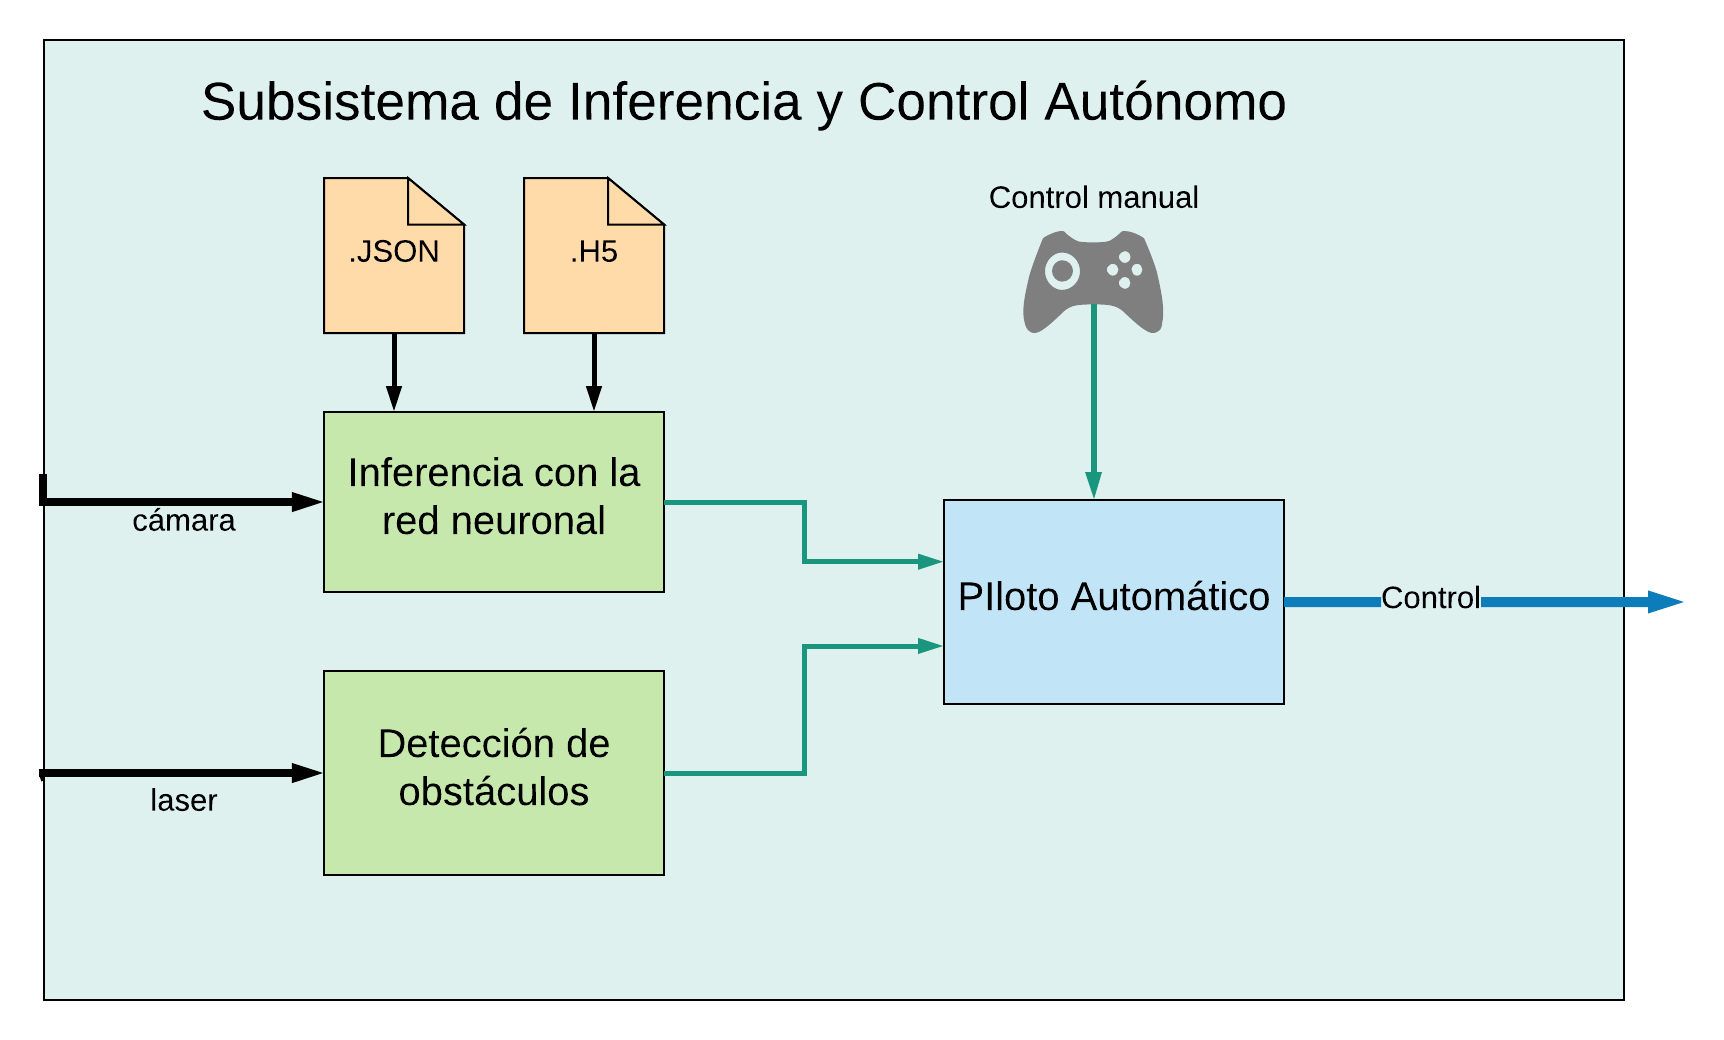
\includegraphics[width=0.85\textwidth]{img/inferencia_esq}
        \caption[Subsistema de Inferencia y Control Autónomo]{Esquema en diagrama de bloques del Subsistema de Inferencia y Control Autónomo. Fuente: Elaboración propia. }
        \label{fig:inferencia_esq}
    \end{figure}

    Este subsistema depende de los otros dos subsistemas de la siguiente manera:
    \begin{itemize}
        \item El subsistema de de adquisión y entrenaminto es el encargado de generar los archivos de la red neuronal que se usan en este subsistema.
        \item El subsistema de control y actuación es el encargado de generar los datos de los sensores y de proveer una plataforma para el control del vehículo.
    \end{itemize}

    El presente proyecto presenta en este subsistema una alternativa a otros métodos tradicionales para sistemas de visión artificial 
    para tareas de control autónomo.

    
\section{Herramientas de software}\label{sec:software}
    \subsection{Robot Operating System - ROS}\label{sec:ros}
    ROS o Sistema Operativo Robótico es un \textit{framework} flexible para desarrollar software para robots. Se compone 
    de una colección de herramientas, librerías y convenciones que tienen el objetivo de simplificar la tarea de crear 
    comportamientos complejos y robustos en plataformas de robótica en general \cite{ros}.

    ROS ha sido construido con el objetivo de hacer accesible el desarrollo de sistemas robóticos mediante el trabajo 
    colaborativo de paquetes y utilidades, su naturaleza modular hace posible que se puedan implementar sistemas pieza 
    por pieza de acuerdo a las necesidades específicas de cada proyecto. Dentro de las facilidades que ROS ofrece, se listan 
    a continuación diversas utilidades que permiten el desarrollo de sistemas con una complejidad elevada.

        \subsubsection{Infraestructura de comunicación}
        En su núcleo, ROS ofrece una interfaz de intercambio de mensajes que provee comunicación inter-procesos y es 
        comunmente referida como el \textit{middleware}. El \textit{middleware} de ROS ofrece las siguientes facilidades:

        \begin{itemize}
            \item Intercambio de mensajes mediante publicación/subscripción y tópicos.
            \item Registro y reproducción de mensajes.
            \item Llamadas a procedimientos del tipo request/response.
            \item Sistema de administración distribuido de parámetros.
        \end{itemize}

        \begin{figure}[!h] 
            \centering
            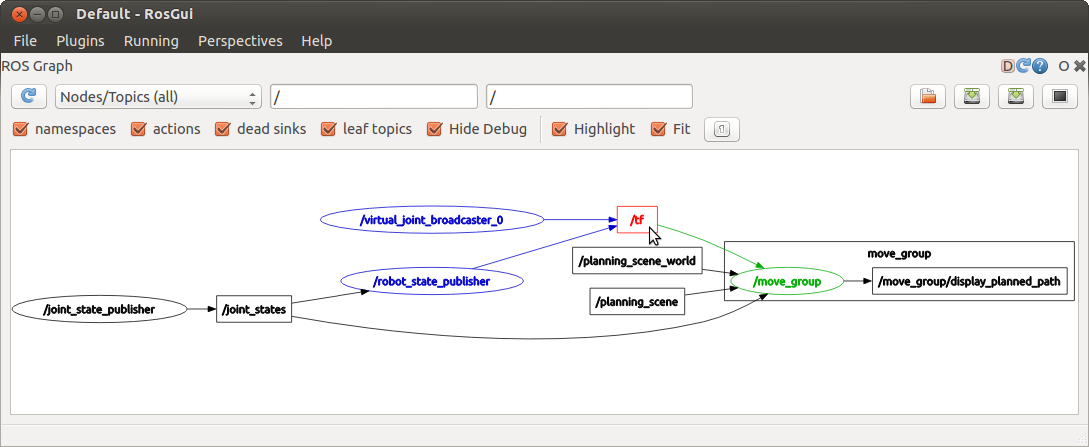
\includegraphics[width=0.75\textwidth]{img/rqtgraph}
            \caption[Diagrama de comunicación de nodos]{Diagrama de comunicación de nodos usando mensajes. Fuente: \cite{roswiki} }
            \label{fig:rqtgraph}
        \end{figure}

        La naturaleza distribuida de ROS y las facilidades que ofrece el \textit{middleware}, hacen que el desarrollo de sistemas 
        robóticos modulares sea una tarea trivial. Aparte de la infraestructura de comunicación, ROS ofrece otras características
        especialmente diseñadas para el desarrollo de robots.
        
        \subsubsection{Nodos de ROS}
        Un nodo en ROS representa a un proceso que se ejecuta de manera independiente y puede aprovechar las facilidades 
        de la infraestructura de comunicación de ROS. Los nodos pueden publicar o subscribirse a uno o varios tópicos. 

        Para que los nodos puedan comunicarse entre sí de manera distribuida y coordinada, existe un proceso especial llamado 
        el ROS master, que registra a todos los nodos y establece los canales de comunicación entre ellos usando los tópicos 
        y mensajes a los cuales los nodos se suscriben y publican. 

        Una característica importante de los Nodos de ROS es que se pueden ejecutar de manera distribuida sobre una red local, 
        lo que implica que se pueden desarrollar sistemas robóticos distribuidos en varias computadoras o estaciones de trabajo. 
        Esto es muy útil en casos donde las características de tamaño, peso y consumo de energía de un robot móvil imposibilita 
        la inclusión de una computadora con las características de memoria y velocidad de procesamiento necesarias para tareas 
        de procesamiento de imágenes o inteligencia artificial, pudiendo ejecutar los nodos con altos requerimientos computacionales 
        en una estación de trabajo remota.

        \begin{figure}[!h] 
            \centering
            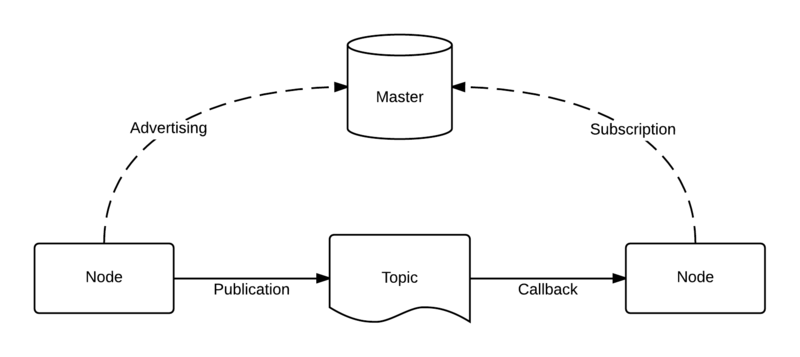
\includegraphics[width=0.75\textwidth]{img/rosnodos}
            \caption[Esquema de la comunicación entre nodos]{Esquema de la comunicación entre nodos. Fuente: \cite{roswiki} }
            \label{fig:rosnodos}
        \end{figure}

        \subsubsection{Características específicas para robótica}
        Adicionalmente a los componentes del \textit{middleware}, ROS tiene a disposición librerías y herramientas específicas 
        para el desarrollo rápido de sistemas robóticos. Algunas de las características más importantes se listan a continuación:

        \begin{itemize}
            \item Definiciones de mensajes estándar para robots.
            \item Lenguaje de descripción de robots URDF\footnote{URDF: Universal Robot Description Format}.
            \item Herramientas de diagnóstico.
            \item Localización.
            \item Mapeo.
            \item Navegación.
            \item Drivers de sensores y actuadores.
        \end{itemize}

        \subsubsection{Herramientas adicionales}
        Una de las características más atractivas de ROS es el conjunto de herramientas para desarrollo. Estas herramientas 
        soportan análisis, depuración y visualización del estado del sistema que esta siendo desarrollado. Los mecanismos presentes
        de publicación y subscripción permiten analizar de manera espontánea el flujo de datos en el sistema. Las herramientas 
        de ROS aprovechan esta característica y se presentan como una colección de herramientas gráficas y de línea de comandos que 
        simplifican el desarrollo y depuración de robots.

        \begin{figure}[!h] 
            \centering
            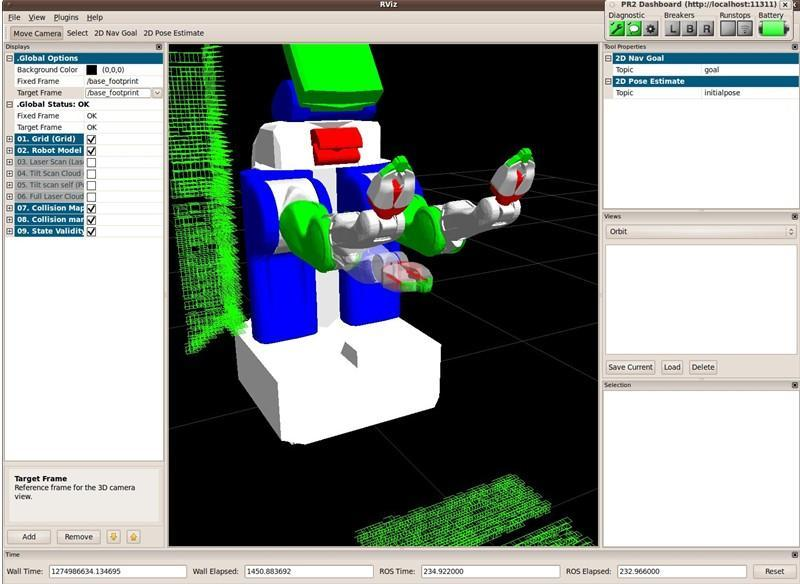
\includegraphics[width=0.75\textwidth]{img/rviz}
            \caption[Interfaz de visualización de ROS rviz]{Interfaz de visualización de ROS rviz. Fuente: \cite{roswiki} }
            \label{fig:rviz}
        \end{figure}

        \begin{itemize}
            \item \textbf{Herramientas de Línea de Comandos.} Permiten el control y depuración de los sistemas 
            de manera remota en una interfaz de línea de comandos. Existen comandos disponibles para ejecutar procesos, 
            analizar tópicos y mensajes, grabar y reproducir sesiones de mensajes y ejecutar servicios.

            \item \textbf{Rviz.} Es una interfaz de visualización de diversas fuentes de datos y modelos de robots. 
            Con la herramienta rviz es posible visualizar diversos tipos de mensajes provenientes de sensores tales 
            como cámaras o sensores láser. También es posible agrupar los distintos tipos de visualizaciones de manera 
            jerárquica en la misma ventana.

            \item \textbf{Rqt.} Rqt es un \textit{framework} para el desarrollo de interfaces gráficas para robots. 
            Con rqt es posible crear interfaces de control o monitoreo de manera gráfica y personalizada usando 
            componentes llamados plugins.

        \end{itemize}


        \subsubsection{Criterios de selección}
        En el marco del presente proyecto y el tiempo establecido para su desarrollo se ha basado la selección del entorno 
        de trabajo en base a los siguientes criterios:
        \begin{itemize}
            \item \textbf{Interfaz de comunicación distribuida.} Es necesario que se puedan desarrollar componentes del sistema 
            de manera independiente y puedan ser ejecutados de la misma manera. ROS ofrece mediante el desarrollo de 
            paquetes y nodos la facilidad de poder ejecutar y comunicar procesos de manera sencilla y distribuida a través
             del intercambio de mensajes.
            \item \textbf{Implementación de funcionalidades comunes.} También se necesita una plataforma con funcionalidades básicas 
            implementadas y disponibles para su uso, esto con el fin de concentrar el tiempo de desarrollo en las funcionalidades del 
            sistema en su conjunto más que en la plataforma sobre la cual se va a desplegar. Se necesitan herramientas reutilizables 
            para evitar lo que comúnmente se denomina como \textit{reinventar la rueda}.
            \item \textbf{Uso libre y código abierto.} ROS es una plataforma de código abierto, lo que permite utilizarlo de manera 
            libre ya sea para proyectos académicos y comerciales. Además, su naturaleza open source permite también realizar cambios 
            o mejoras en su funcionalidad de manera sencilla. El uso libre es importante dado que en entornos académicos normalmente 
            no se cuenta con la facilidad de adquirir licencias de software privativo. El uso libre también permite el desarrollo por 
            parte de investigadores independientes y estudiantes que no pertenecen a alguna institución que pueda apoyarlos financieramente.
            \item \textbf{Facilidad de uso.} El entorno de trabajo debe tener la facilidad de ser accesible para personas con un 
            conocimiento previo en electrónica y programación. Tanto los lenguajes de programación como las herramientas de desarrollo, 
            compilación y despliegue tienen que estar disponibles y ser fáciles de utilizar.
            \item \textbf{Compatibilidad con herramientas externas.} En el marco del proyecto y la aplicación de los conceptos de 
            visión artificial y aprendizaje profundo. El entorno de trabajo debe ser compatible o poder extender sus funcionalidades 
            con otros entornos dedicados al procesamiento de imágenes y visión artificial como a entornos y librerías 
            para el desarrollo y entrenamiento de redes neuronales. 
            \item \textbf{Interfaces con sistemas de bajo nivel y tiempo real.} Es necesario que la plataforma también 
            sea compatible con el desarrollo de sistemas embebidos y de tiempo real para el control de actuadores y 
            sensores que no se pueden conectar a una PC directamente.
        \end{itemize}

        Es en este sentido que se ha escogido usar al \textit{framework} ROS como plataforma de desarrollo para los distintos módulos 
        del sistema. Cabe resaltar que ROS no es la única plataforma para desarrollar robots, y algunas alternativas se detallan en la 
        Tabla(\ref{tbl:frameworks}) donde se puede analizar las características de cada una. 

      
        % Please add the following required packages to your document preamble:
        % \usepackage{booktabs}
        \begin{table}[!h]
            \begin{tabular}{@{}|c|c|c|c|c|c|@{}}
            \toprule
            \textbf{Nombre}                                             & \textbf{\begin{tabular}[c]{@{}c@{}}Interfaz de \\ Comunicación\\ Distribuida\end{tabular}} & \textbf{\begin{tabular}[c]{@{}c@{}}Sistema de \\ compilación\end{tabular}} & \textbf{\begin{tabular}[c]{@{}c@{}}Gestión de \\ paquetes\end{tabular}} & \textbf{\begin{tabular}[c]{@{}c@{}}Drivers de \\ bajo nivel\end{tabular}} & \textbf{\begin{tabular}[c]{@{}c@{}}Lenguajes de \\ programación\end{tabular}} \\ \midrule
            ROS                                                         & SI                                                                                         & SI                                                                         & SI                                                                      & SI                                                                        & \begin{tabular}[c]{@{}c@{}}C++\\ Python\\ Java\end{tabular}                   \\ \midrule
            YARP                                                        & SI                                                                                         & NO                                                                         & NO                                                                      & SI                                                                        & C++                                                                           \\ \midrule
            ROCK                                                        & SI                                                                                         & SI                                                                         & NO                                                                      & NO                                                                        & C++                                                                           \\ \midrule
            MRTP                                                        & NO                                                                                         & NO                                                                         & NO                                                                      & SI                                                                        & C++                                                                           \\ \midrule
            Player                                                      & SI                                                                                         & SI                                                                         & NO                                                                      & NO                                                                        & C++                                                                           \\ \midrule
            \begin{tabular}[c]{@{}c@{}}Robotics \\ Library\end{tabular} & NO                                                                                         & NO                                                                         & NO                                                                      & SI                                                                        & C++                                                                           \\ \bottomrule
            \end{tabular}
            \caption{Tabla comparativa de características entre distintas plataformas y librerías para desarrollo de sistemas robóticos. Fuente: Elaboración propia} % TODO: referencia
            \label{tbl:frameworks}
            \end{table}

        ROS se usa de manera extensiva en el desarrollo del presente proyecto para las siguientes tareas:

        \begin{itemize}
            \item En el subsistema de control y actuación como una interfaz común de intercambio de mensajes para el control de los motores presentes en el prototipo, así como también en la recuperación de los datos de los sensores. Estas interfaces están implementadas como nodos de ROS.
            \item En el subsistema de adquisición de datos y entrenamiento como una herramienta de captura de información del control manual y la cámara, tomando en cuenta las estampas de tiempo y sincronización para cada mensaje de ROS.
            \item En el subsistema de inferencia y control autónomo como la plataforma sobre la cual se definen los distintos controladores como nodos de ROS y el programa del piloto automático como un árbitro entre los mensajes de los distintos controladores. 
            \item En todo el sistema como la interfaz de comunicación distribuida a través del intercambio de mensajes entre el prototipo y la estación de trabajo remota.
        \end{itemize}

    \subsection{Tensorflow}
    Tensorflow es una librería para cálculos numéricos que funciona en base a grafos de flujo de datos Figura(\ref{fig:grafotf}). Las operaciones matemáticas 
    se representan como nodos en el grafo y los vértices representan matrices de datos multidimensionales o tensores que fluyen de 
    un nodo a otro  \cite{tensorflow2015-whitepaper}. Debido a esta implementación, los grafos pueden ejecutarse de manera distribuida en varias CPU o GPU. Las operaciones 
    matemáticas están disponibles para utilizar en la librería y sus implementaciones estan altamente optimizadas, lo que permite 
    aprovechar al máximo el hardware disponible.

    \begin{figure}[!h] 
        \centering
        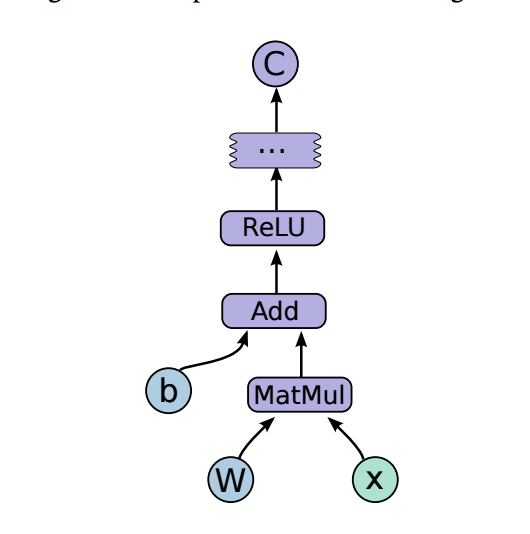
\includegraphics[width=0.55\textwidth]{img/grafotf}
        \caption[Ejemplo de un grafo de cómputo utilizado en Tensorflow]{Ejemplo de un grafo de cómputo utilizado en Tensorflow. Fuente: \cite{asjad_2016} }
        \label{fig:grafotf}
    \end{figure}

    Tensorflow se ha hecho popular por la facilidad con la que se puede implementar la arquitectura de una red neuronal usando grafos
    de cómputo y por la optimización de los algoritmos usados. Actualmente, Tensorflow representa el estándar en la implementación de 
    redes neuronales profundas tanto en la academia como la industria. 

    Otra de las características de Tensorflow es que presenta una API en el lenguaje de programación Python, lo que permite el desarrollo
    de redes neuronales de manera muy sencilla e intuitiva. 

    En el presente proyecto, se utiliza Tensorflow como librería base para la implementación de la red neuronal tanto en la etapa de 
    entrenamiento como en la etapa de inferencia. El entrenamiento e inferencia se implementan usando los algoritmos de Tensorflow 
    optimizados para GPU\footnote{GPU: Graphics Processing Unit o Unidad de Procesamiento de Gráficos} de la marca Nvidia.
    % TODO: agregar referencia a otros capitulos

    Es importante listar algunos términos que se usarán en el contexto de este proyecto, relacionados exclusivamente con la implementación 
    de la red neuronal convolucional correspondiente con el sistema fin a fin que se implementa. 
    \begin{itemize}
        \item \textbf{Tensor:} Es una generalización de un vector o una matriz en dimensiones superiores. Internamente, 
        Tensorflow representa tensores como arreglos n-dimensionales de tipos de datos base, como ser Int32 o Float64.

        \item \textbf{Variable: } Refiere a la manera de presentar el estado persistente que se puede manipular por el 
        programa o grafo de cómputo. Una variable contiene internamente un tensor con valores que se pueden modificar 
        mediante operaciones. Las variables en Tensorflow comunmente se utilizan para representar a los pesos o parámetros 
        de la red neuronal.

        \item \textbf{Grafo:} Un grafo es un objeto de Tensorflow que contiene la información acerca de la estructura 
        del grafo de cómputo que se va a utilizar. Contiene la información de las distintas operaciones y las conexiones 
        entre las mismas por las que fluyen los tensores. La estructura del grafo debe ser declarada antes de su ejecución.

        \item \textbf{Operación:} Una operación representa a un nodo en el grafo, tiene como entrada uno o varios 
        tensores y produce como salida uno o varios tensores. Las operaciones definen los cálculos que se realizan entre 
        tensores como ser una multiplicación de matrices o una operación de convolución, entre otras.
    \end{itemize}

    En el siguiente ejemplo, se puede observar la definición de un grafo de cómputo básico en Tensorflow:

    \begin{lstlisting}[title={Ejemplo de un programa escrito con Tensorflow},captionpos=b,language=Python]
        import tensorflow as tf 
            #definicion de variables
            input1 = tf.Variable(3.0) 
            input2 = tf.Variable(2.0)
            input3 = tf.Variable(5.0)

            #definicion de las operaciones y el grafo
            intermed = tf.add(input2,input3)
            mul = tf.mul(input1,intermed)

            #ejecucion de las operaciones 
            with tf.Session() as sess:
                result = sess.run([mul,intermed])
                print(result) 

    \end{lstlisting}

    \subsection{Keras}
    Keras es una librería para la definición e implementación de redes neuronales de alto nivel escrita en Python y compatible con 
    diversas plataformas de cómputo tales como Tensorflow, CNTK o Theano \cite{chollet2015keras}. Esta librería ha sido desarrollada con el objetivo de 
    facilitar la experimentación y prototipado rápido de modelos de aprendizaje profundo. Las características de la librería que 
    la convierten en una opción viable en el desarrollo de modelos de aprendizaje profundo son las siguientes:

    \begin{itemize}
        \item Permite el prototipado rápido a través de su facilidad de uso, modularidad y capacidad de ser extendida.
        \item Soporta la definición de redes neuronales recurrentes y redes neuronales convolucionales. La última categoría es la más importante para el presente proyecto.
        \item Soporta la ejecución tanto en CPU como en GPU.
    \end{itemize}

    Keras se basa en la definición de redes neuronales en base a capas. Existe una clase especial de modelo llamado \textit{Sequential} que 
    representa básicamente una red neuronal feedforward (Sección(\ref{sec:feedforward})). En un modelo \textit{Sequential} se define 
    a la red en base a las capas de las que se compone, cada capa puede tener distinta naturaleza y características. 
    
    Además de la definición de las capas, Keras también cuenta con implementaciones de algoritmos de optmización y funciones de costo 
    comunmente utilizadas en trabajos de investigación en la actualidad, lo cual facilita todavía más el desarrollo de modelos de 
    redes neuronales. En el siguiente 
    ejemplo, se puede apreciar la definición de la red neuronal de dos capas definida en la Ecuación(\ref{eq:reddoscapas}) con 32 unidades en 
    la capa de entrada y 4 unidades en la capa de salida, con una función de costo de entropía cruzada categórica y el algoritmo de 
    optimización de \textit{Stochastic Gradient Descent}:

    \begin{lstlisting}[title={Ejemplo de una red neuronal usando la librería Keras},captionpos=b,language=Python]
        from keras.models import Sequential
        from keras.layers import Dense, Activation

        modelo = Sequential()
        #primera capa
        model.add(Dense(32), input_dim=128)
        model.add(Activation('sigmoid'))
        #segunda capa
        model.add(Dense(4), input_dim=128)
        model.add(Activation('sigmoid'))
        #optimizador y funcion de costo
        model.compile(loss='categorical_crossentropy',
                            optimizer='sgd',
                            metrics=['accuracy']
                            )
    \end{lstlisting}

    \subsection{ARM Mbed}
    Mbed es una iniciativa llevada adelante por ARM que brinda un conjunto de herramientas de hardware y software para el 
    desarrollo de dispositivos IoT (Internet de las Cosas). Mbed es un ecosistema de desarrollo sobre el cual se pueden 
    desarrollar aplicaciones con microcontroladores con arquitectura ARM provenientes de distintos fabricantes \cite{mbed}. La 
    característica principal de Mbed es la sencillez de su uso y la amplia gama de librerías disponibles para distintos componentes 
    de hardware como sensores, actuadores o displays. ARM Mbed presenta las siguientes características clave para el desarrollo 
    de sistemas embebidos de manera rápida y favorables al contexto del presente proyecto:

    \begin{itemize}
        \item Variedad de placas de desarrollo de microcontroladores ARM de distintos fabricantes.
        \item Una interfaz de programación común a todos los microcontroladores y fabricantes para la interfaz con 
        periféricos embebidos.
        \item Un compilador en línea donde se pueden crear, compilar y desplegar proyectos.
        \item Variedad de librerías para dispositivos como sensores, módulos de comunicación o actuadores.
        \item El uso del lenguaje C++ con la especificación completa hace posible el desarrollo orientado 
        a objetos para aprovechar altos niveles de abstracción en la programación.
        \item La capacidad de generación de símbolos de depuración para su ejecución paso por paso con el fin de 
        identificar \textit{bugs} en tiempo de ejecución.
        \item La compatibilidad con la librería Rosserial que hace posible poder comunicar al microcontrolador 
        con el \textit{middleware} de ROS de manera directa usando un puerto serial.
    \end{itemize}

    Mbed se usará como la plataforma para el desarrollo del control de tiempo real en el subsistema de control y actuación 
    ya que ofrece todas las facilidades en cuanto a librerías y potencia computacional necesarias para esta tarea. En la 
    Tabla(\ref{tbl:frameworks}) se puede observar una tabla comparativa entre diversas plataformas de desarrollo embebido 
    consideradas para el presente proyecto.


    \begin{table}[!h]
        \begin{tabular}{|c|c|c|c|c|}
        \hline
        \textbf{Plataforma} & \textbf{Arquitectura}                                                          & \textbf{Lenguaje} & \textbf{\begin{tabular}[c]{@{}c@{}}Nivel de \\ abstracción\end{tabular}} & \textbf{Enfoque}                                                          \\ \hline
        Arduino             & AVR - 8 bits                                                                   & Wiring (C++)      & Alto                                                                     & \begin{tabular}[c]{@{}c@{}}Hobby, Arte \\ y Educación\end{tabular}        \\ \hline
        Mbed                & ARM - 32 bits                                                                  & C++               & Alto                                                                     & \begin{tabular}[c]{@{}c@{}}IoT, Sistemas \\ de tiempo real\end{tabular}   \\ \hline
        Energia             & \begin{tabular}[c]{@{}c@{}}TI MSP430 - 16 bits\\ TI ARM - 32 bits\end{tabular} & Wiring (C++)      & Alto                                                                     & \begin{tabular}[c]{@{}c@{}}Hobby, Sistemas \\ de tiempo real\end{tabular} \\ \hline
        Freedom E SDK       & RISC V - 32 bits                                                               & C                 & Bajo                                                                     & \begin{tabular}[c]{@{}c@{}}Sistemas de \\ tiempo real\end{tabular}        \\ \hline
        libOpenCM3          & ARM - 32 bits                                                                  & C                 & Bajo                                                                     & \begin{tabular}[c]{@{}c@{}}Sistemas de \\ tiempo real\end{tabular}        \\ \hline
        \end{tabular}
    \end{table}

    Una de las plataformas de desarrollo más utilizadas en la actualidad es Arduino, pese a haberse considerado esta plataforma 
    por su disponibilidad, popularidad y gran soporte por la comunidad se ha detectado algunas limitaciones en la misma 
    que hacen que no se la pueda recomendar para desarrollos académicos:

    \begin{itemize}
        \item Si bien el nivel de abstracción facilita la introducción a los microcontroladores para personas 
        sin experiencia, oculta varios aspectos referidos al hardware de los periféricos del microcontrolador que 
        escapan de control. Esta falta de control de bajo nivel puede ocasionar fallos y situaciones en las que no 
        se pueda predecir con seguridad el comportamiento de un sistema. La predictibilidad es una característica 
        fundamental en cualquier sistema de tiempo real.

        \item El lenguaje de programación usado Wiring es un subconjunto del lenguaje C++ que carece de varias 
        funcionalidades y no permite el desarrollo de clases con herencia y polimorfismo implementadas de manera adecuada.

        \item El entorno de desarrollo integrado porporcionado, el Arduino IDE, es un entorno demasiado limitado 
        para desarrollos de proyectos de mediana y gran envergadura.

        \item La falta de capacidades de depuración, una limitación de la propia arquitectura AVR imposibilita el 
        análisis del comportamiento en tiempo de ejecución del código y la identificación de posibles \textit{bugs} 
        que puedan aparecer. Esta característica es de vital importancia para el desarrollo de sistemas de seguridad crítica.

    \end{itemize}


\section{Herramientas de hardware}\label{sec:hardware}
Se han seleccionado diversas herramientas de hardware para la implementación del sistema de conducción autónoma. Dichas herramientas
corresponden con la base física electrónica sobre la cual se ejecutarán las tareas de los tres subsistemas. Se procede a detallar 
las herramientas utilizadas en el diseño del sistema.

    \subsection{Plataforma de tiempo real}\label{sec:mcu}
    La interfaz de más bajo nivel del sistema es el de la interacción con los actuadores de los motores del prototipo. Esta 
    interfaz debe tener la capacidad de poder comunicarse con la OBC y además de poder cumplir ciertos requisitos de ejecución 
    en tiempo real. Estos requisitos de tiempo real hace que tal comportamiento no se pueda implementar en la OBC pues la misma 
    usa un sistema operativo basado en el kernel GNU/Linux, el cual no cuenta por defecto con capacidades de tiempo real dura. 
    Por tanto, se ha establecido la necesidad de utilizar una plataforma embebida con una arquitectura más sencilla y con un 
    nivel de predictibilidad mucho mayor al de la OBC. En este caso se usará un microcontrolador con arquitectura ARM Cortex M3.

    La arquitectura ARM se ha popularizado bastante en los últimos años principalmente por su característica de tener un conjunto 
    reducido de instrucciones y sencillez en la microarquitectura del procesador en comparación con otras arquitecturas comúnmente 
    encontradas en servidores y computadoras personales como son X86 o PowerPC. Esta simplificación en la arquitectura y la reproducción
    del conjunto de instrucciones ha permitido que los dispositivos basados en ARM puedan reducir dramáticamente el consumo de 
    energía sin degradar demasiado el rendimiento. Es por eso que ARM, en la actualidad se constituye como la principal arquitectura en 
    dispositivos móviles y de bajo consumo con cientos de millones de dispositivos usándola alrededor del mundo.

    Sin embargo, el desarrollo e implemtación de esta arquitectura se ha dirigido bastante hacia procesadores de aplicación, presentes
    en dispositivos como teléfonos inteligentes o tablets. Es por eso que ARM ha presentado una familia de procesadores ARM que estan
    orientados exclusivamente al desarrollo de sistemas embebidos con capacidades de tiempo real y ultra bajo conmo de energía. Esta 
    familia es la familia ARM Cortex-M que cuenta con varias características que la hacen ideal para el desarrollo del sistema en tiempo 
    real requerido para la interfaz con los actuadores del presente proyecto.

    Por su parte, dado que ARM no fabrica chips sino mas bien vende licencias de la arquitectura a distintas marcas fabricantes, existe 
    una multitud de procesadores usando esta arquitectura de distintos fabricantes, entre los cuales se puede mencionar a ST Microelectronics,
    Texas Instruments, Nordic, entre otros. Para el presente proyecto, se necesita que el microcontrolador pueda cumplir con las 
    siguientes características. 

    \begin{itemize}
        \item Al menos un puerto de comunicación serial.
        \item Periféricos capaces de generar señales PWM o con los recursos necesarios para emular PWM por software.
        \item Memoria de datos y de programa suficiente para poder incluir la librería de Rosserial en el mismo.
        \item Capacidades de depuración y ejecución paso por paso para la identificación de fallas.
        \item Operación en niveles de tensión compatibles con la OBC.
    \end{itemize}

    Es por eso que se ha seleccionado la placa de desarrollo de ST Microelectronics Mucleo f303k8 (Figura(\ref{fig:nucleo})), tomando en cuenta 
    que cumple con todos los requisitos anteriormente establecidos y además cuenta con las siguientes características:


    \begin{figure}[!h] 
        \centering
        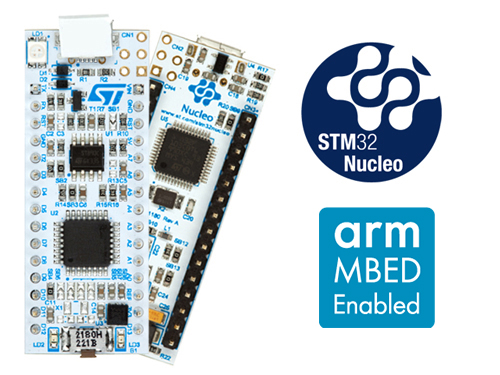
\includegraphics[width=0.55\textwidth]{img/nucleo}
        \caption[Placa de desarrollo Nucleof303k8 de ST Microelectronics]{Placa de desarrollo Nucleof303k8 de ST Microelectronics. Fuente: \cite{nucleof303} }
        \label{fig:nucleo}
    \end{figure}


    \begin{itemize}
        \item Circuito grabador-depurador en la placa, STlink V2.
        \item Capacidades de comunicación seria mediante USB para un puerto de comunicación seria virtual e intefaz de depuración.
        \item Múltiples fuentes de alimentación.
        \item Leds indicadores.
        \item Factor de forma compatible con varios entornos de desarrollo electrónico.
    \end{itemize}


    Se han explorado diversas alternativas al uso de la placa de desarrollo Nucleof303k8 para la implementación de este módulo. En 
    la Tabla(\ref{tbl:mcucomp}) se pueden apreciar las características de varias placas de desarrollo embebido candidatas disponibles en el mercado.

    % Please add the following required packages to your document preamble:
    % \usepackage{booktabs}
    % \usepackage{graphicx}
    \begin{table}[]
        \centering
        \resizebox{\textwidth}{!}{%
        \begin{tabular}{@{}|c|c|c|c|c|c|c|@{}}
        \toprule
        \textbf{Modelo} & \textbf{Arquitectura}                                                & \textbf{\begin{tabular}[c]{@{}c@{}}RAM\\ (KB)\end{tabular}} & \textbf{\begin{tabular}[c]{@{}c@{}}ROM\\ (KB)\end{tabular}} & \textbf{\begin{tabular}[c]{@{}c@{}}Frecuencia de \\ Reloj (MHz)\end{tabular}} & \textbf{\begin{tabular}[c]{@{}c@{}}Canales \\ PWM\end{tabular}} & \textbf{\begin{tabular}[c]{@{}c@{}}Entorno de \\ Trabajo\end{tabular}} \\ \midrule
        Atmega328p      & AVR (8 bits)                                                         & 2                                                           & 32                                                          & 16                                                                            & 6 (8 bits)                                                      & \begin{tabular}[c]{@{}c@{}}Arduino,\\ Atmel Studio\end{tabular}        \\ \midrule
        PIC18f2550      & PIC (8 bits)                                                         & 2                                                           & 32                                                          & 48                                                                            & 2 (8 bits)                                                      & MPlab                                                                  \\ \midrule
        STM32f103c8     & \begin{tabular}[c]{@{}c@{}}ARM \\ CortexM3\\  (32 bits)\end{tabular} & 20                                                          & 64                                                          & 72                                                                            & 12 (16 bits)                                                    & \begin{tabular}[c]{@{}c@{}}STM32 HAL,\\ Arduino\end{tabular}           \\ \midrule
        STM32f303k8     & \begin{tabular}[c]{@{}c@{}}ARM \\ CortexM4f\\ (32 bits)\end{tabular} & 16                                                          & 64                                                          & 72                                                                            & 8                                                               & \begin{tabular}[c]{@{}c@{}}STM32 HAL,\\ \textbf{Mbed}\end{tabular}              \\ \bottomrule
        \end{tabular}%
        }
        \caption{Comparación de características de microcontroladores disponibles. Fuente: Elaboración propia.}
        \label{tbl:mcucomp}
        \end{table}

    

    El microcontrolador utilizado, el STM32F303k8 pertenece a la familia de microcontroladores con arquitectura ARM Cortex M4f del 
    fabricante ST Microelectronics. Es parte de la gama de microcontroladores f3 de la famila STM32 que esta orientado al procesamiento 
    de señales pues cuenta con un procesador de 32 bits con una unidad de punto flotante que le permite realizar cálculos y operaciones 
    con números decimales de manera eficiente. Las características del microcontrolador seleccionado se listan a continuación:

    % Please add the following required packages to your document preamble:
    % \usepackage{booktabs}
    % \usepackage{graphicx}
    \begin{table}[]
        \centering
        \resizebox{0.8\textwidth}{!}{%
        \begin{tabular}{@{}|r|l|@{}}
        \toprule
        \textbf{Núcleo}                     & ARM Cortex M4 de 32 bits con unidad de punto flotante \\ \midrule
        \textbf{Frecuencia de reloj}        & 72 MHz Máximo                                         \\ \midrule
        \textbf{Voltaje de operación}       & 2.0 V a 3.6 V (nominal: 3.3 V)                        \\ \midrule
        \textbf{Memoria de datos}           & 16 KB SRAM                                            \\ \midrule
        \textbf{Memoria de programa}        & 64 KB FLASH                                           \\ \midrule
        \textbf{Timers Disponibles}         & 7                                                     \\ \midrule
        \textbf{Interfaces de Comunicación} & SPI/I2S, I2C, USART, CAN                              \\ \midrule
        \textbf{Periféricos adicionales}    & GPIO (con interrupciones), ADC, DAC, RTC              \\ \bottomrule
        \end{tabular}%
        }
        \caption{Características técnicas del microcontrolador STM32f303k8. Fuente: \cite{nucleof303}}
        \label{tbl:mcuspecs}
        \end{table}

    % \begin{itemize}
    %     \item \textbf{Núcleo: } ARM CortexM4 de 32 bits con unidad de punto flotante.
    %     \item \textbf{Frecuencia de reloj: } 72 MHz máximo.
    %     \item \textbf{Voltaje de operación: } desde 2.0 V hasta 3.6V (nominal 3.3V).
    %     \item \textbf{Memoria de datos: } 16 KB SRAM.
    %     \item \textbf{Memoria de programa: } 64 KB FLASH.
    %     \item \textbf{Timers: } 7.
    %     \item \textbf{Interfaces de comunicación: } SPI/I2S, I2C, USART, CAN.
    %     \item \textbf{Periféricos adicionales: } GPIO (Con interrupciones), ADC, DAC, RTC.
    % \end{itemize}

    Como se puede observar en la Tabla(\ref{tbl:mcuspecs}), las características del microcontrolador cumplen con los requisitos establecidos tanto en interfaces 
    de comunicación como en cantidad y variedad de periféricos para una posterior extensión de la funcionalidad. Por otra parte, 
    tal como se puede apreciar en la Tabla(\ref{tbl:mcucomp}), esta placa es compatible con el entorno de trabajo de programación 
    ARM Mbed, y con la librería Rosserial.

    \subsection{Computadora de Abordo - OBC}

    En el caso del hardware necesario para la OBC, se requiere un sistema capaz ejecutar un sistema operativo GNU/Linux completo 
    con el fin de poder correr el software necesario para el control, comunicación y adquisición de imágenes de una cámara, necesarias
    para el funcionamiento correcto del sistema en su conjunto. Es en este sentido que se ha optado por el uso de una \textit{Single Board Computer}
    o Computadora de Una Placa, que refiere a placas de desarrollo con todas las características de una computadora de escritorio, es decir:
    procesador, memoria y periféricos incorporados. Existe gran variedad de SBC en el mercado con distintas características y aplicaciones 
    objetivo. En la Tabla(\ref{tbl:sbc}) se puede apreciar una comparación de varias SBC disponibles en el mercado y sus características 
    relevantes al presente proyecto.

   % Please add the following required packages to your document preamble:
    % \usepackage{booktabs}
    % \usepackage{graphicx}
    \begin{table}[]
        \centering
        \resizebox{\textwidth}{!}{%
        \begin{tabular}{@{}|c|c|c|c|c|c|c|c|@{}}
        \toprule
        \textbf{Placa}                                                & \textbf{Procesador}                                                          & \textbf{RAM} & \textbf{LAN} & \textbf{\begin{tabular}[c]{@{}c@{}}Conexión\\ Inalámbrica\end{tabular}} & \textbf{\begin{tabular}[c]{@{}c@{}}Soporte y\\ documentación\end{tabular}} & \textbf{\begin{tabular}[c]{@{}c@{}}Precio\\ (\$us)\end{tabular}} & \textbf{\begin{tabular}[c]{@{}c@{}}Soporta \\ ROS\end{tabular}} \\ \midrule
        \begin{tabular}[c]{@{}c@{}}Asus \\ Tinkerboard\end{tabular}   & 4x A17 @ 1.8 GHz                                                             & 2 GB         & GBe          & \begin{tabular}[c]{@{}c@{}}Wifi\\ Bluetooth\end{tabular}                & Regular                                                                    & 60                                                               & NO                                                              \\ \midrule
        Odroid X4u                                                    & \begin{tabular}[c]{@{}c@{}}4x A15 @ 2.0 GHz +\\ 4x A7 @ 1.4 GHz\end{tabular} & 2 GB         & GBe          & NO                                                                      & Bueno                                                                      & 85                                                               & SI                                                              \\ \midrule
        \begin{tabular}[c]{@{}c@{}}Raspberry Pi\\ zero W\end{tabular} & 1x A8 @ 1GHz                                                                 & 512 MB       & NO           & \begin{tabular}[c]{@{}c@{}}Wifi\\ Bluetooth\end{tabular}                & Muy bueno                                                                  & 20                                                               & NO                                                              \\ \midrule
        \begin{tabular}[c]{@{}c@{}}Beaglebone \\ Black\end{tabular}   & 1x A8 @ 1GHz                                                                 & 512 MB       & Fast         & NO                                                                      & Bueno                                                                      & 60                                                               & SI                                                              \\ \midrule
        Raspberry Pi 3b+                                              & 4x A53 @ 1.4 GHz                                                             & 1 GB         & Fast         & \begin{tabular}[c]{@{}c@{}}Wifi\\ Bluetooth\end{tabular}                & Muy bueno                                                                  & 40                                                               & SI                                                              \\ \midrule
        Rock64                                                        & 4x A53 @ 1.5 GHz                                                             & 2 GB         & GBe          & NO                                                                      & Regular                                                                    & 35                                                               & NO                                                              \\ \midrule
        Beaglebone Blue                                               & 1x A8 @ 1GHz                                                                 & 512 MB       & no           & \begin{tabular}[c]{@{}c@{}}Wifi\\ Bluetooth\end{tabular}                & Regular                                                                    & 80                                                               & SI                                                              \\ \bottomrule
        \end{tabular}%
        }
        \caption{Tabla comparativa de SBC's disponibles en el mercado. Fuente: Elaboración propia.}
        \label{tbl:sbc}
        \end{table}


    La placa seleccionada como OBC debe cumplir ciertas características específicas para este proyecto:


    \begin{itemize}
        \item Factor de forma: Dimensiones y peso reducidos para poder ser incorporada en el prototipo.
        \item Consumo de energía: Bajo consumo de energia, es necesario que pueda ser alimentado por baterías disponibles en el mercado.
        \item Compatibilidad de software: La placa debe poder correr una distribución completa de GNU/Linux reciente, compatible con ROS.
        \item Compatibilidad de hardware: La placa debe poder conectarse de manera nativa con el microcontrolador elegido para la interfaz de tiempo real. Contar con puertos USB y puertos USART.
        \item Interfaz con una cámara: Debe contar también con una forma de conectar y adquirir imágenes provenientes de una cámara digital.
        \item Comunicación inalámbrica: Se necesita la capacidad de poder conectarse a una red LAN mediante Wifi, ya sea con un módulo incorporado o un accesorio externo.
        \item Precio y disponibilidad: Es importante que el precio no sea demasiado elevado para poder garantizar la replicabilidad del proyecto, así como también la disponibilidad en el mercado.
        \item Soporte y documentación: Es necesario que la placa cuente con una buena documentación y soporte de la comunidad o fabricante para que el resolver problemas relativos a la placa no tome demasiado tiempo.
    \end{itemize}

    \begin{figure}[!h] 
        \centering
        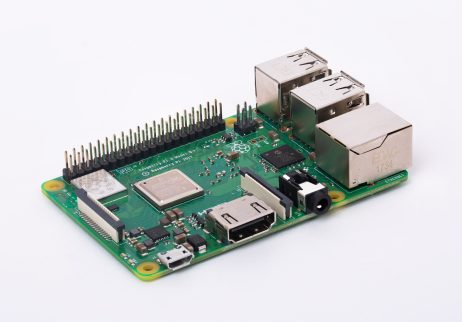
\includegraphics[width=0.75\textwidth]{img/raspi}
        \caption[Placa de desarrollo Raspberry Pi 3 model B+]{Placa de desarrollo Raspberry Pi 3 model B+. Fuente: \cite{raspi} }
        \label{fig:raspi}
    \end{figure}

    Al final, se ha seleccionado a la placa Raspberry Pi 3B+ (Figura(\ref{fig:raspi})) para la OBC del proyecto pues cuenta con todas las características 
    necesarias para poder ejecutar las herramientas de software requeridas y también cuenta con los periféricos adecuados para 
    comunicarse con la plataforma de tiempo real. La placa en cuestión cuenta con las características listadas en la Tabla(\ref{tbl:raspispecs})

    
    % Please add the following required packages to your document preamble:
    % \usepackage{booktabs}
    % \usepackage{graphicx}
    \begin{table}[]
        \centering
        \resizebox{0.85\textwidth}{!}{%
        \begin{tabular}{@{}|r|l|@{}}
        \toprule
        \textbf{SoC}                        & Broadcom BCM2837B0                                                  \\ \midrule
        \textbf{CPU}                        & 1.4 GHz 64-bit quad core ARM Cortex-A53                             \\ \midrule
        \textbf{RAM}                        & 1 GB LPDDR2 SDRAM                                                   \\ \midrule
        \textbf{Wifi}                       & Dual-band 802.11ac wireless LAN (2.4GHz and 5GHz ) y Bluetooth 4.2. \\ \midrule
        \textbf{Video}                      & VideoCore IV 3D                                                     \\ \midrule
        \textbf{USB}                        & 2.0, 4 puertos                                                      \\ \midrule
        \textbf{Interfaces de Comunicación} & SPI/I2S, I2C, USART                                                 \\ \midrule
        \textbf{Interfaces de cámara}       & USB webcam, CSI                                                     \\ \bottomrule
        \end{tabular}%
        }
        \caption{Características de la placa Raspberry Pi 3 model B+. Fuente: \cite{raspi}}
        \label{tbl:raspispecs}
        \end{table}


    % \begin{itemize}
    %     \item Soc\footnote{System on Chip}: Broadcom BCM2837B0, Cortex-A53 (ARMv8) 64-bit.
    %     \item CPU: 1.4GHz 64-bit quad-core ARM Cortex-A53 CPU.
    %     \item RAM: 1GB LPDDR2 SDRAM.
    %     \item Wifi: Dual-band 802.11ac wireless LAN (2.4GHz and 5GHz ) and Bluetooth 4.2.
    %     \item Video: VideoCore IV 3D.
    %     \item USB: 2.0, 4 ports.
    % \end{itemize}


    \subsection{Estación de trabajo}
    La estación de trabajo se usa para realizar el entrenamiento de la red neuronal en el subsistema de adquisición de datos y 
    entrenamiento. Dada la naturaleza de la tarea del entrenamiento de una red neuronal, esta estación de trabajo presenta algunos 
    requerimientos especiales: 

    \begin{itemize}
        \item Sistema Operativo: Se necesita un sistema operativo basado en GNU/Linux compatible con ROS, Tensorflow y Keras.
        \item GPU: Con la finalidad de acelerar el tiempo de entrenamiento de la red neuronal convolucional, es altamente recomendable contar con una GPU de la marca Nvidia, compatible con Tensorflow.
        \item Wifi: Es necesaria una conexión Wifi inalámbrica para poder comunicarse con el prototipo tanto en la etapa de adquisición de datos y entrenamiento, como en la de inferencia para el monitoreo remoto.
    \end{itemize}
    
    Considerando los requisitos, las características de la estación de trabajo seleccionada se listan en la Tabla(\ref{tbl:pcspecs}). 

    % Please add the following required packages to your document preamble:
    % \usepackage{booktabs}
    % \usepackage{graphicx}
    \begin{table}[!h]
        \centering
        \resizebox{0.85\textwidth}{!}{%
        \begin{tabular}{@{}|r|l|@{}}
        \toprule
        \textbf{Modelo}            & MSI GL62 6qd                                                              \\ \midrule
        \textbf{CPU}               & Intel Core i7-6700HQ @ 2.6 GHz x 8 núcleos                                \\ \midrule
        \textbf{RAM}               & 16 GB DDR4 @ 2133 MHz                                                     \\ \midrule
        \textbf{Wifi}              & Intel Dual-band 802.11ac wireless LAN (2.4GHz and 5GHz ) y Bluetooth 4.2. \\ \midrule
        \textbf{GPU}               & Nvidia GTX950m 2GB VRAM                                                   \\ \midrule
        \textbf{Sistema Operativo} & Ubuntu 18.04 Linux 4.15                                                   \\ \bottomrule
        \end{tabular}%
        }
        \caption{Características de la estación de trabajo seleccionada. }
        \label{tbl:pcspecs}
        \end{table}

    La estación de trabajo se utilizará para el entrenamiento de la red neuronal pues cuenta con los requisitos de memoria RAM y una 
    GPU compatible para la paralelización de los algoritmos de entrenamiento de la librería Tensorflow. Estos algoritmos incluyen 
    el cálculo de gradientes de toda la red y el ajuste de los pesos optimizados para ejecutarse de forma paralela dada la naturaleza
    matricial de las operaciones involucradas.

    \subsection{Sensores}
    Un aspecto fundamental en el desarrollo de un sistema de conducción autónoma es la elección adecuada de los sensores, que son 
    los dispositivos que recolectan datos acerca del estado del entorno del vehículo. En el presente proyecto, se están utilizando 
    dos tipos de sensores: Una cámara para recuperar las imágenes de la carretera y un sensor de proximidad para detectar obstáculos 
    al frente del vehículo.
        \subsubsection{Cámara}\label{sec:raspicam}
        En el caso de la cámara, existen diversas opciones para poder recuperar imágenes del entorno variando desde la calidad 
        de la imagen que recuperan, velocidad de captura, rango dińamico y otras características. Sin embargo, se debe tomar 
        en cuenta algunas limitaciones impuestas por el sistema en su conjunto:

        \begin{itemize}
            \item La capacidad de procesamiento es limitada en la OBC al tratarse de un sistema de bajo consumo de energía y dimensiones reducidas.
            \item La capacidad de transferencia en la red está limitada a especificaciones de los módulos de comunicación inalámbrica, reduciendo la cantidad de información que puede ser compartida entre la estación de trabajo remota y el prototipo.
            \item El consumo de energía debe ser limitado al estar el sistema alimentado por baterías.
        \end{itemize}

        Considerando las limitaciones planteadas, se puede reducir las opciones de cámaras a utilizar en este proyecto a cámaras web 
        y al módulo de cámara de Raspberry Pi (Figura(\ref{fig:raspicam})). El último ítem cuenta con algunas características muy interesantes que la hacen una 
        candidata idónea para su uso en el presente proyecto que se pueden observar en la Tabla(\ref{tbl:raspicamspecs}).

        \begin{figure}[!h] 
            \centering
            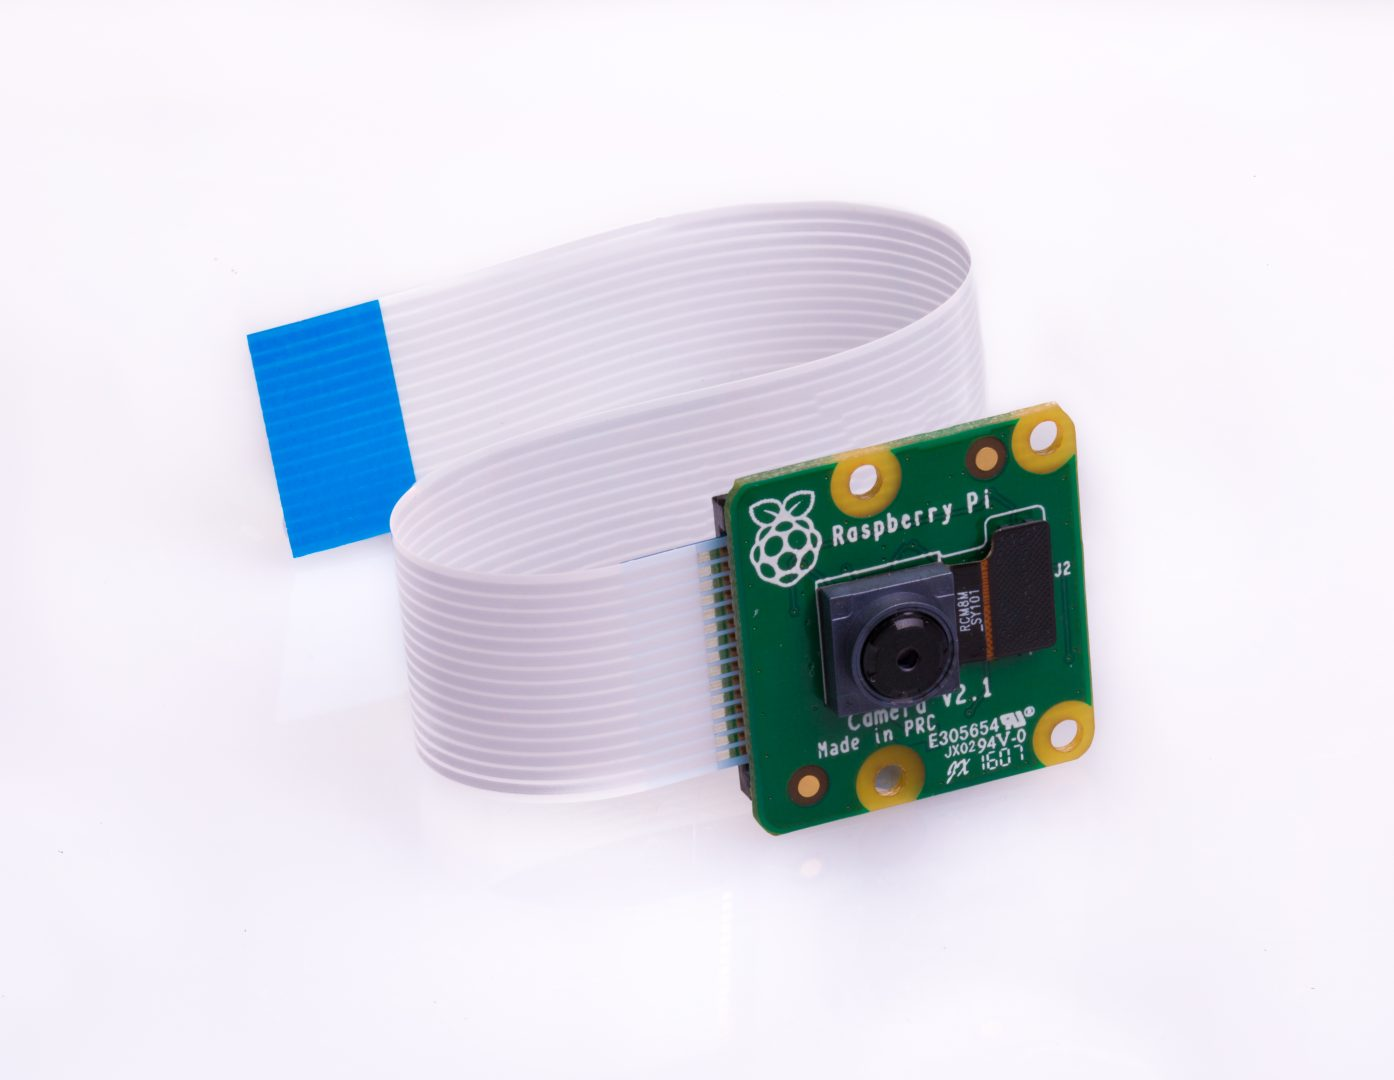
\includegraphics[width=0.65\textwidth]{img/raspicam}
            \caption[Raspberry Pi Camera Module V2]{Raspberry Pi Camera Module V2. Fuente: \cite{raspicam} }
            \label{fig:raspicam}
        \end{figure}

        % Please add the following required packages to your document preamble:
        % \usepackage{booktabs}
        % \usepackage{graphicx}
        \begin{table}[!h]
            \centering
            \resizebox{0.5\textwidth}{!}{%
            \begin{tabular}{@{}|r|l|@{}}
            \toprule
            \textbf{Sensor}      & Sony IMX219 8 megapixeles          \\ \midrule
            \textbf{Resolución}  & Fotografía: 3280x2464 Video: 1080p \\ \midrule
            \textbf{Framerate}   & 1080p@30Hz, 720p@60Hz, 640p@90Hz   \\ \midrule
            \textbf{Interfaz}    & CSI                                \\ \midrule
            \textbf{Dimensiones} & 25mm x 23mm x 9mm                  \\ \midrule
            \textbf{Peso}        & 3.4g                               \\ \bottomrule
            \end{tabular}%
            }
            \caption{Características de la Raspberry Pi Camera Module V2. Fuente: \cite{raspicam}}
            \label{tbl:raspicamspecs}
            \end{table}
        
        Dentro de las razones por la cual se ha escogido a la Raspberry Pi Camera Module V2 se tiene la capacidad de 
        grabar video a 90 cuadros por segundo, una característica importante para poder incrementar el tiempo de muestreo del 
        bucle de control. En segundo lugar, la cámara utiliza una interfaz CSI que puede conectarse directamente a la placa Raspberry
        Pi tal como se puede apreciar en la Figura(\ref{fig:raspicamconn})
        
        \begin{figure}[!h] 
            \centering
            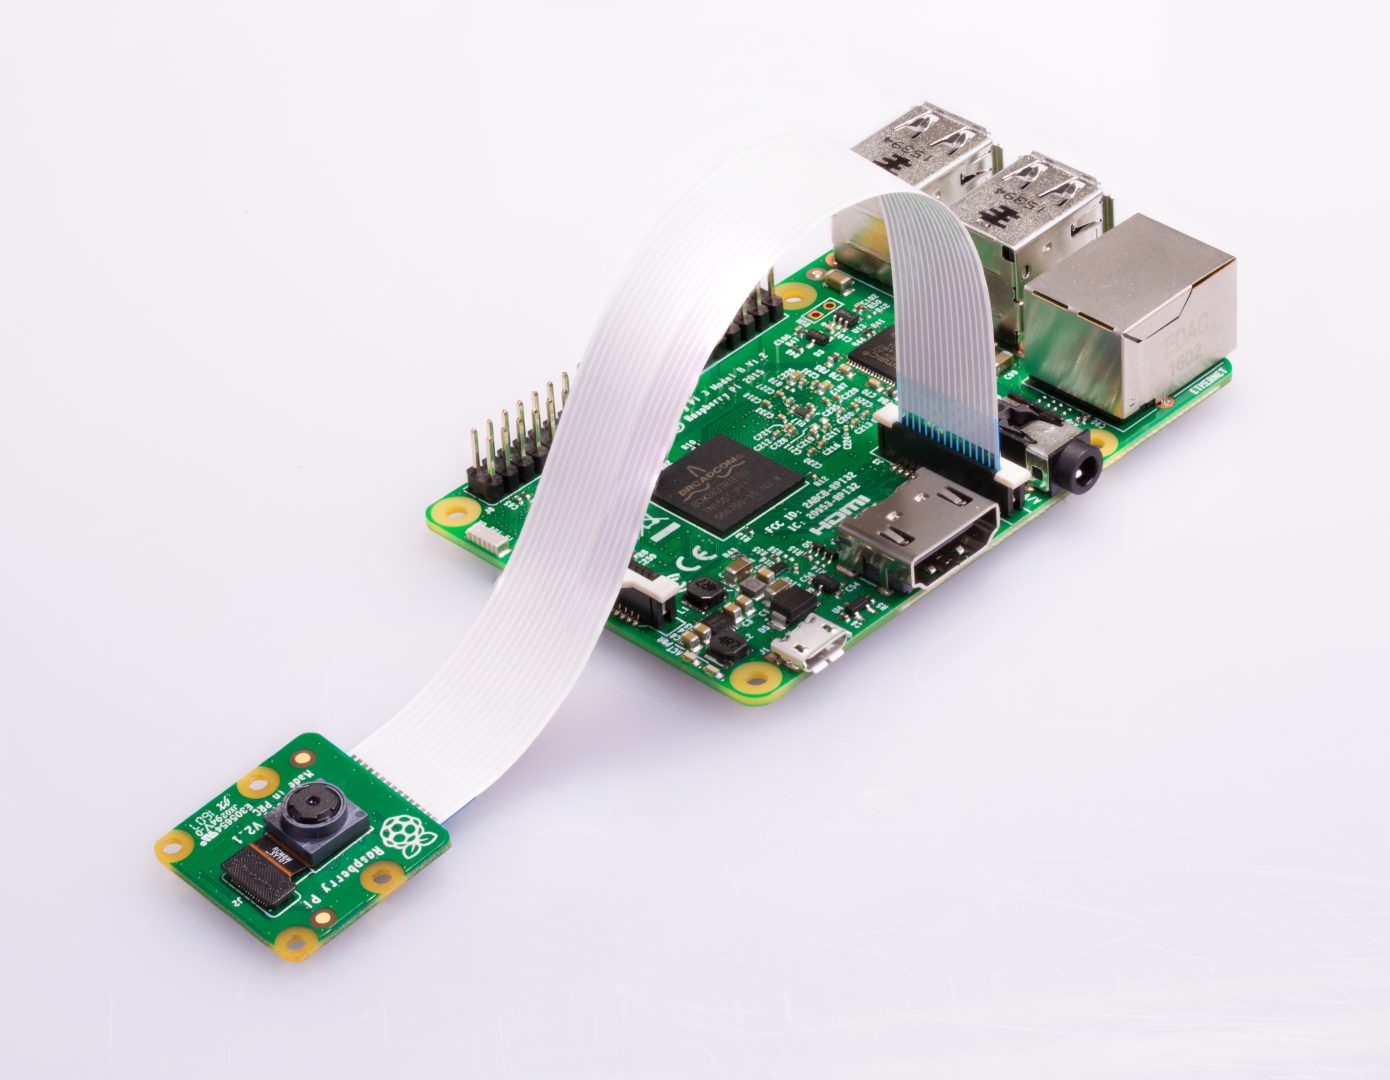
\includegraphics[width=0.65\textwidth]{img/raspicamconn}
            \caption[Conexión de la Camera Module V2]{Conexión de la Camera Module V2 con una placa Raspberry Pi. Fuente: \cite{raspicam} }
            \label{fig:raspicamconn}
        \end{figure}

        La ventaja de poderse conectar con la placa mediante la interfaz CSI es que los \textit{frames} provenientes del sensor 
        se procesan directamente en la GPU de la Raspberry Pi y no así en la GPU, esto gracias a la disponibilidad de los 
        controladores correspondientes para la Camera Module V2. Esto no es posible cuando se trata de cámaras USB o webcam 
        debido a que los controladores de las mismas procesan los \textit{frames} en la CPU haciendo su procesamiento más lento 
        y ocupando mayor cantidad de ciclos de CPU.

        \subsubsection{Sensor de proximidad}\label{sec:laser}
        El segundo sensor necesario para la implementación del sistema de control autónomo es un sensor de proximidad que 
        sea capaz de detectar la presencia y distancia de obstáculos que se presenten en frente del vehículo. Este sensor 
        también debe ser compatible con los protocolos de comunicación o periféricos disponibles en la OBC y en el sistema 
        de control de tiempo real.

        \begin{figure}[!h] 
            \centering
            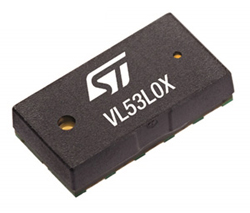
\includegraphics[width=0.35\textwidth]{img/laser}
            \caption[Sensor VL53L0X de ST Microelectronics]{Conexión de la Camera Module V2 . Fuente: \cite{laser} }
            \label{fig:laser}
        \end{figure}

        El sensor seleccionado para la tarea es el sensor VL53L0X (Figura(\ref{fig:laser})) de ST Microelectronics. El cual es un sensor óptico de 
        proximidad con láser que usa el principio ToF{\textit{Time of Flight}} o Tiempo de Vuelo, se basa en el tiempo 
        en el que la luz tarda en reflejarse de la superficie para calcular la distancia dada una velocidad constante de la luz 
        mediante la siguiente fórmula:
        
        \begin{equation}\label{eq:tof}
            d = \frac{c}{t_{vuelo} / 2}
        \end{equation}

        donde $d$ es la distancia recorrida y $c$ es la velocidad de la luz. Se puede apreciar una ilustración del principio 
        de funcionamiento del sensor en la Figura(\ref{fig:tof}). 
        
        \begin{figure}[!h] 
            \centering
            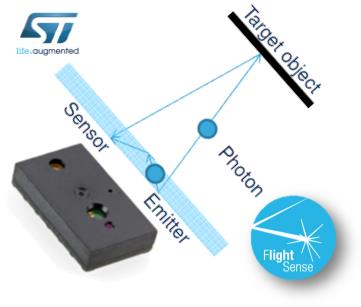
\includegraphics[width=0.35\textwidth]{img/tof}
            \caption[Ilustración del principio ToF]{Ilustración del principio ToF. Fuente: \cite{laser} }
            \label{fig:tof}
        \end{figure}

        Los sensores láser que usan el principio ToF tienen varias ventajas en relación a otro tipo de sensores como los sensores 
        ultrasónicos, o los sensores infrarrojos refractarios. En primer lugar, son inmunes a interferencia sonora o ultrasónica 
        y son más robustos en cuanto a la variedad de superfices sobre las cuales se puede reflejar el haz de luz. El sensor 
        VL53L0X se constituye como una opción favorable para el desarrollo del presente proyecto y por eso se ha elegido. Sus 
        características se detallan en la Tabla(\ref{tbl:laserspecs}).

        % Please add the following required packages to your document preamble:
        % \usepackage{booktabs}
        % \usepackage{graphicx}
        \begin{table}[!h]
            \centering
            \resizebox{0.65\textwidth}{!}{%
            \begin{tabular}{@{}|r|l|@{}}
            \toprule
            \textbf{Láser}                     & 940 nm Clase 1 (seguro a los ojos) \\ \midrule
            \textbf{Rango efectivo}            & 30 mm  - 1200 mm                   \\ \midrule
            \textbf{Interfaz de comunicación}  & I2C @ 400 KHz                      \\ \midrule
            \textbf{Tiempo de muestreo mínimo} & 20 ms                              \\ \midrule
            \textbf{Voltaje de operación}      & 2.6 V  - 3.5 V (nominal: 3.3 V)    \\ \bottomrule
            \end{tabular}%
            }
            \caption{Características del sensor VL53L0X. Fuente: \cite{vl53l0x}}
            \label{tbl:laserspecs}
            \end{table}
        
            
        El sensor se ha utilizado en una placa de desarrollo o \textit{Breakout Board} que incluye un regulador de tensión 
        y los pines de comunicación correspondientes para su conexión a la SBC. La información proveniente del sensor 
        de proximidad será recuperada y procesada mediante un nodo de ROS de manera que se pueda integrar al sistema 
        en su conjunto.
            
            \begin{figure}[] 
                \centering
                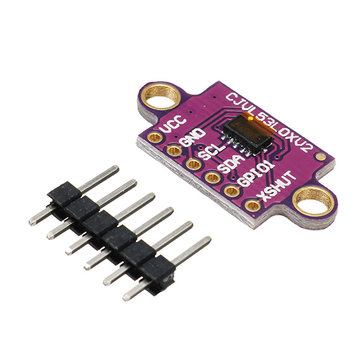
\includegraphics[width=0.45\textwidth]{img/laserbreak}
                \caption[Breakout Board para el sensor VL53L0X]{Breakout Board para el sensor VL53L0X. Fuente: \cite{laser} }
                \label{fig:laserboard}
            \end{figure}
    
\section{Subsistema de Control y actuación}\label{sec:control}

El subsistema de control y actuación representa la base fundamental sobre la cual se desarrolla el resto del proyecto. De acuerdo 
con la naturaleza del mismo, se pretende implementar una plataforma flexible y modular sobre la cual se pueda controlar el 
prototipo de múltiples maneras, partiendo desde un modo teleoperado básico donde un operador humano tiene el control 
de todos los grados de libertad del vehículo, pasando por un modo híbrido hasta un modo autónomo donde los comandos de 
control son generados por un programa que procesa los datos provenientes de los sensores y otras fuentes externas.

La finalidad del subsistema es brindar una interfaz amigable y flexible para el control de los actuadores del vehículo. Esta 
interfaz se logra gracias a la infraestructura de ROS mediante el envío de mensajes. Los mensajes utilizados en este subsistema 
son los mensajes Twist, que se utilizan comúnmente para expresar la velocidad del movimiento de un robot o vehículo en ROS. Se ha
escogido el mensaje Twist porque presenta de manera muy conveniente la separación entre la velocidad lineal o 
la tracción del vehículo y la desviación o la dirección. 

La interfaz con el \textit{middleware} de ROS se logra a través de un paquete llamado \lstinline{rosserial}, que crea un nodo especial 
que es capaz de enviar mensajes mediante el puerto serial a sistemas embebidos que no cuentan con una conexión ethernet. De esta 
manera, el control de los actuadores es transparente a cualquier otro nodo en la red haciendo posible que se pueda controlar 
el vehículo de distintas maneras, incluso desde nodos ejecutados de manera remota en estaciones de trabajo en la red local.


    \subsection{Módulo de potencia en tiempo real}
    El prototipo cuenta con dos actuadores para la tracción y la dirección respectivamente. En el caso de la tracción, se 
    utiliza un motor de corriente contínua de imán permanente en conjunción con un controlador de potencia capaz de manipular 
    al mismo. El control del motor se basa en la combinación de dos pines de dirección y un pin correspondiente con la velocidad 
    que es controlada mediante una señal modulada en ancho de pulso o PWM. 

    Por su parte, el control de la dirección se realiza mediante el uso de un servomotor dimensionado adecuadamente para la aplicación 
    que controla el ángulo de las ruedas delanteras. El ángulo de las ruedas define el ICC (Sección(\ref{sec:ruedas})), que a su vez 
    define el radio de giro mínimo en base al máximo rango en el que puede variar el ángulo de las ruedas delanteras. En la 
    Figura(\ref{fig:actuadores}) se puede apreciar el prototipo y la disposición de los actuadores del mismo.

    \begin{figure}[!h] 
        \centering
        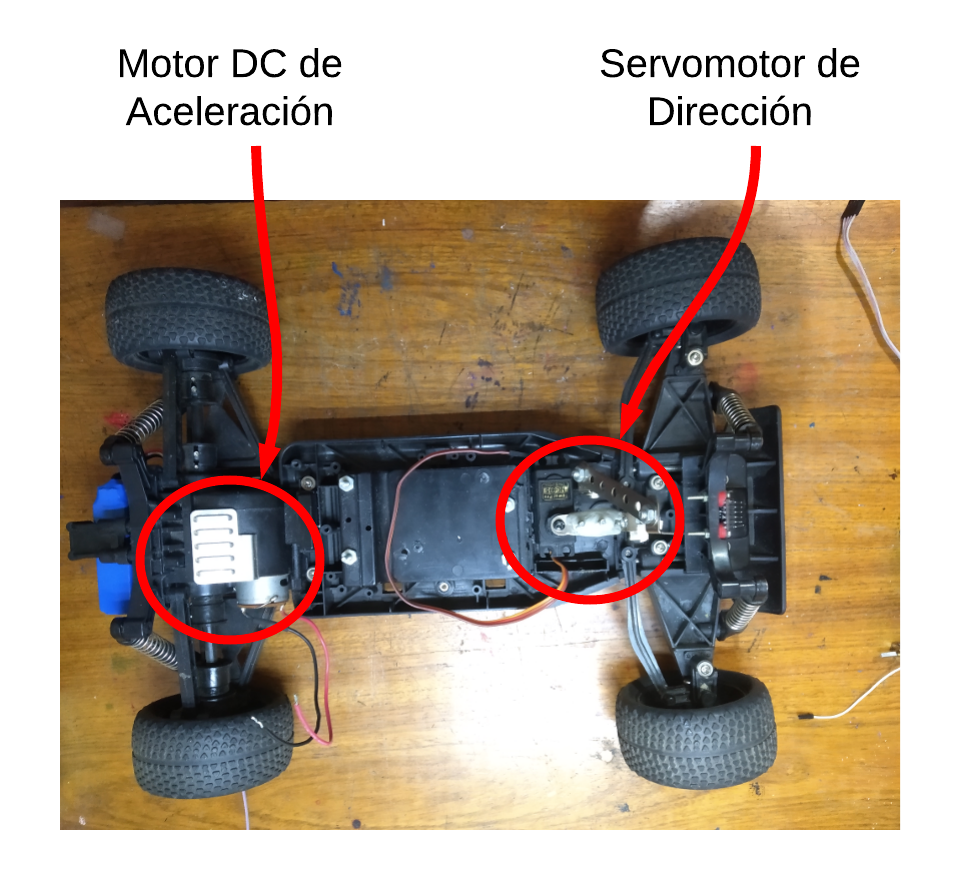
\includegraphics[width=0.75\textwidth]{img/actuadores}
        \caption[Prototipo del vehículo]{Prototipo del vehículo. Fuente: Elaboración propia. }
        \label{fig:actuadores}
    \end{figure}

    El servomotor que se encarga de la dirección del vehículo se puede apreciar en la Figura(\ref{fig:servo}) y el motor DC de aceleración 
    en la Figura(\ref{fig:dcmotor}).

    \begin{figure}[!h] 
        \centering
        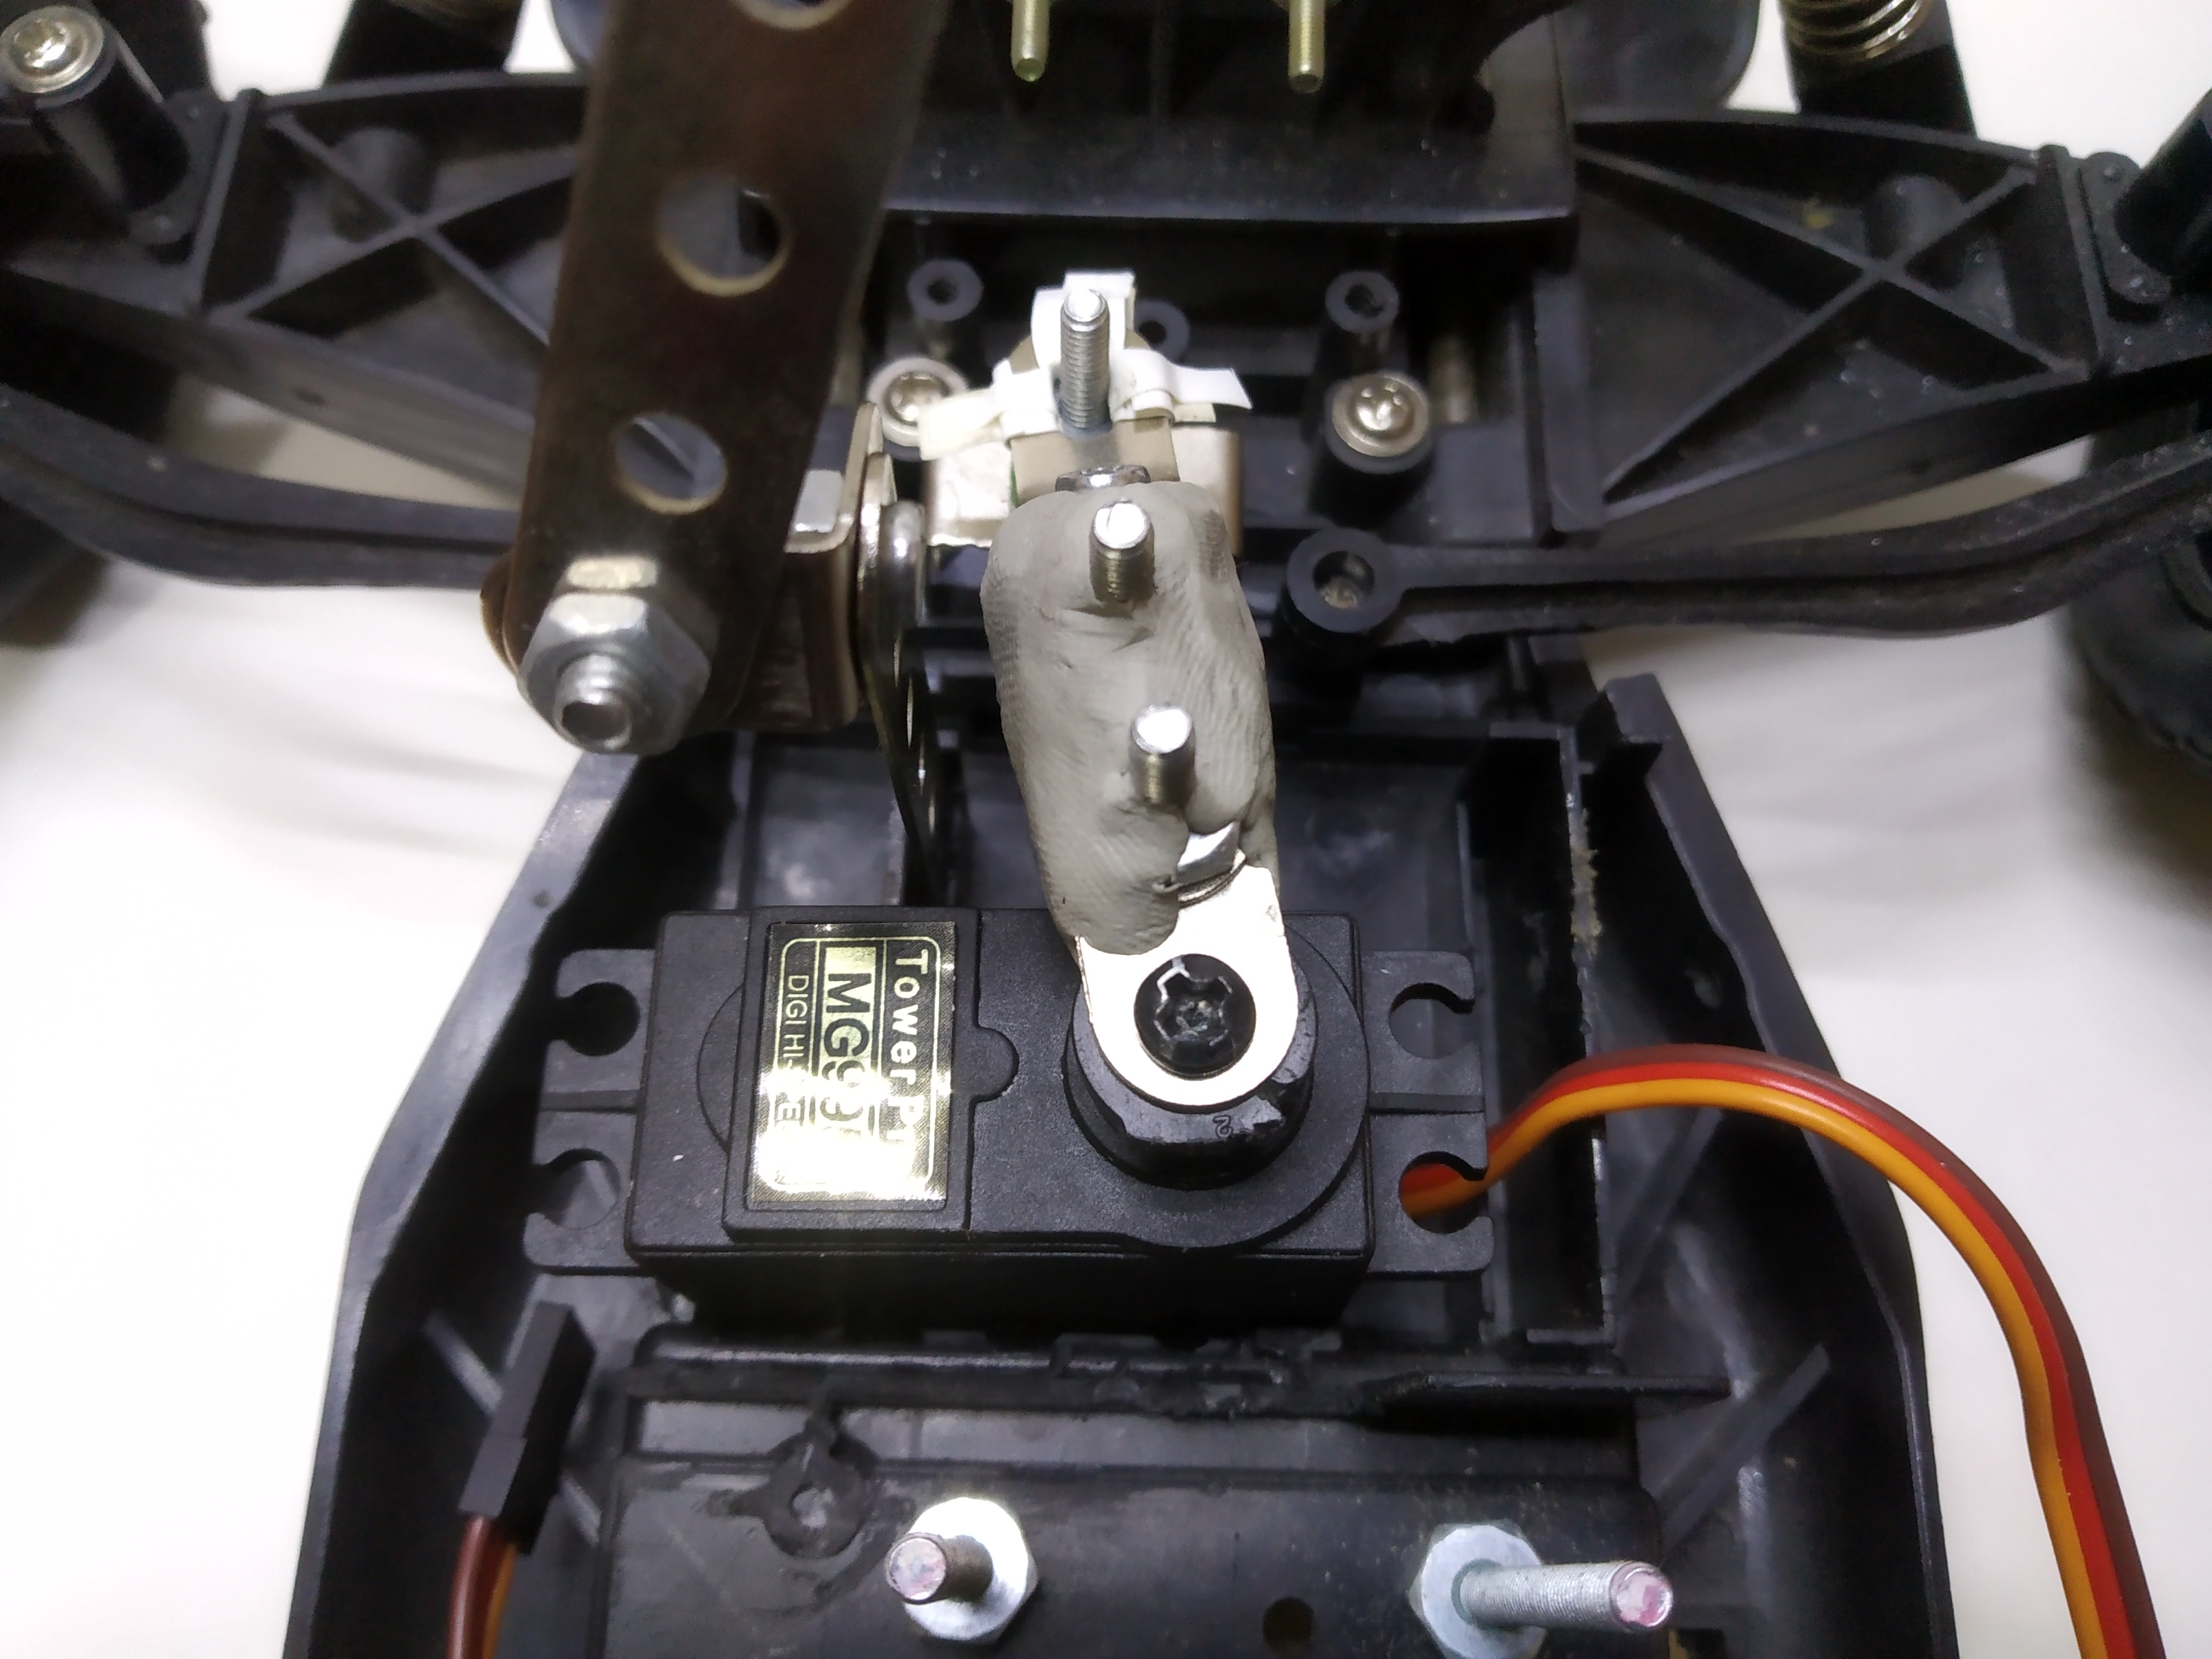
\includegraphics[width=0.55\textwidth]{img/servo}
        \caption[Fotografía del servomotor de dirección]{Fotografía del servomotor de dirección. Fuente: Elaboración propia. }
        \label{fig:servo}
    \end{figure}

    \begin{figure}[!h] 
        \centering
        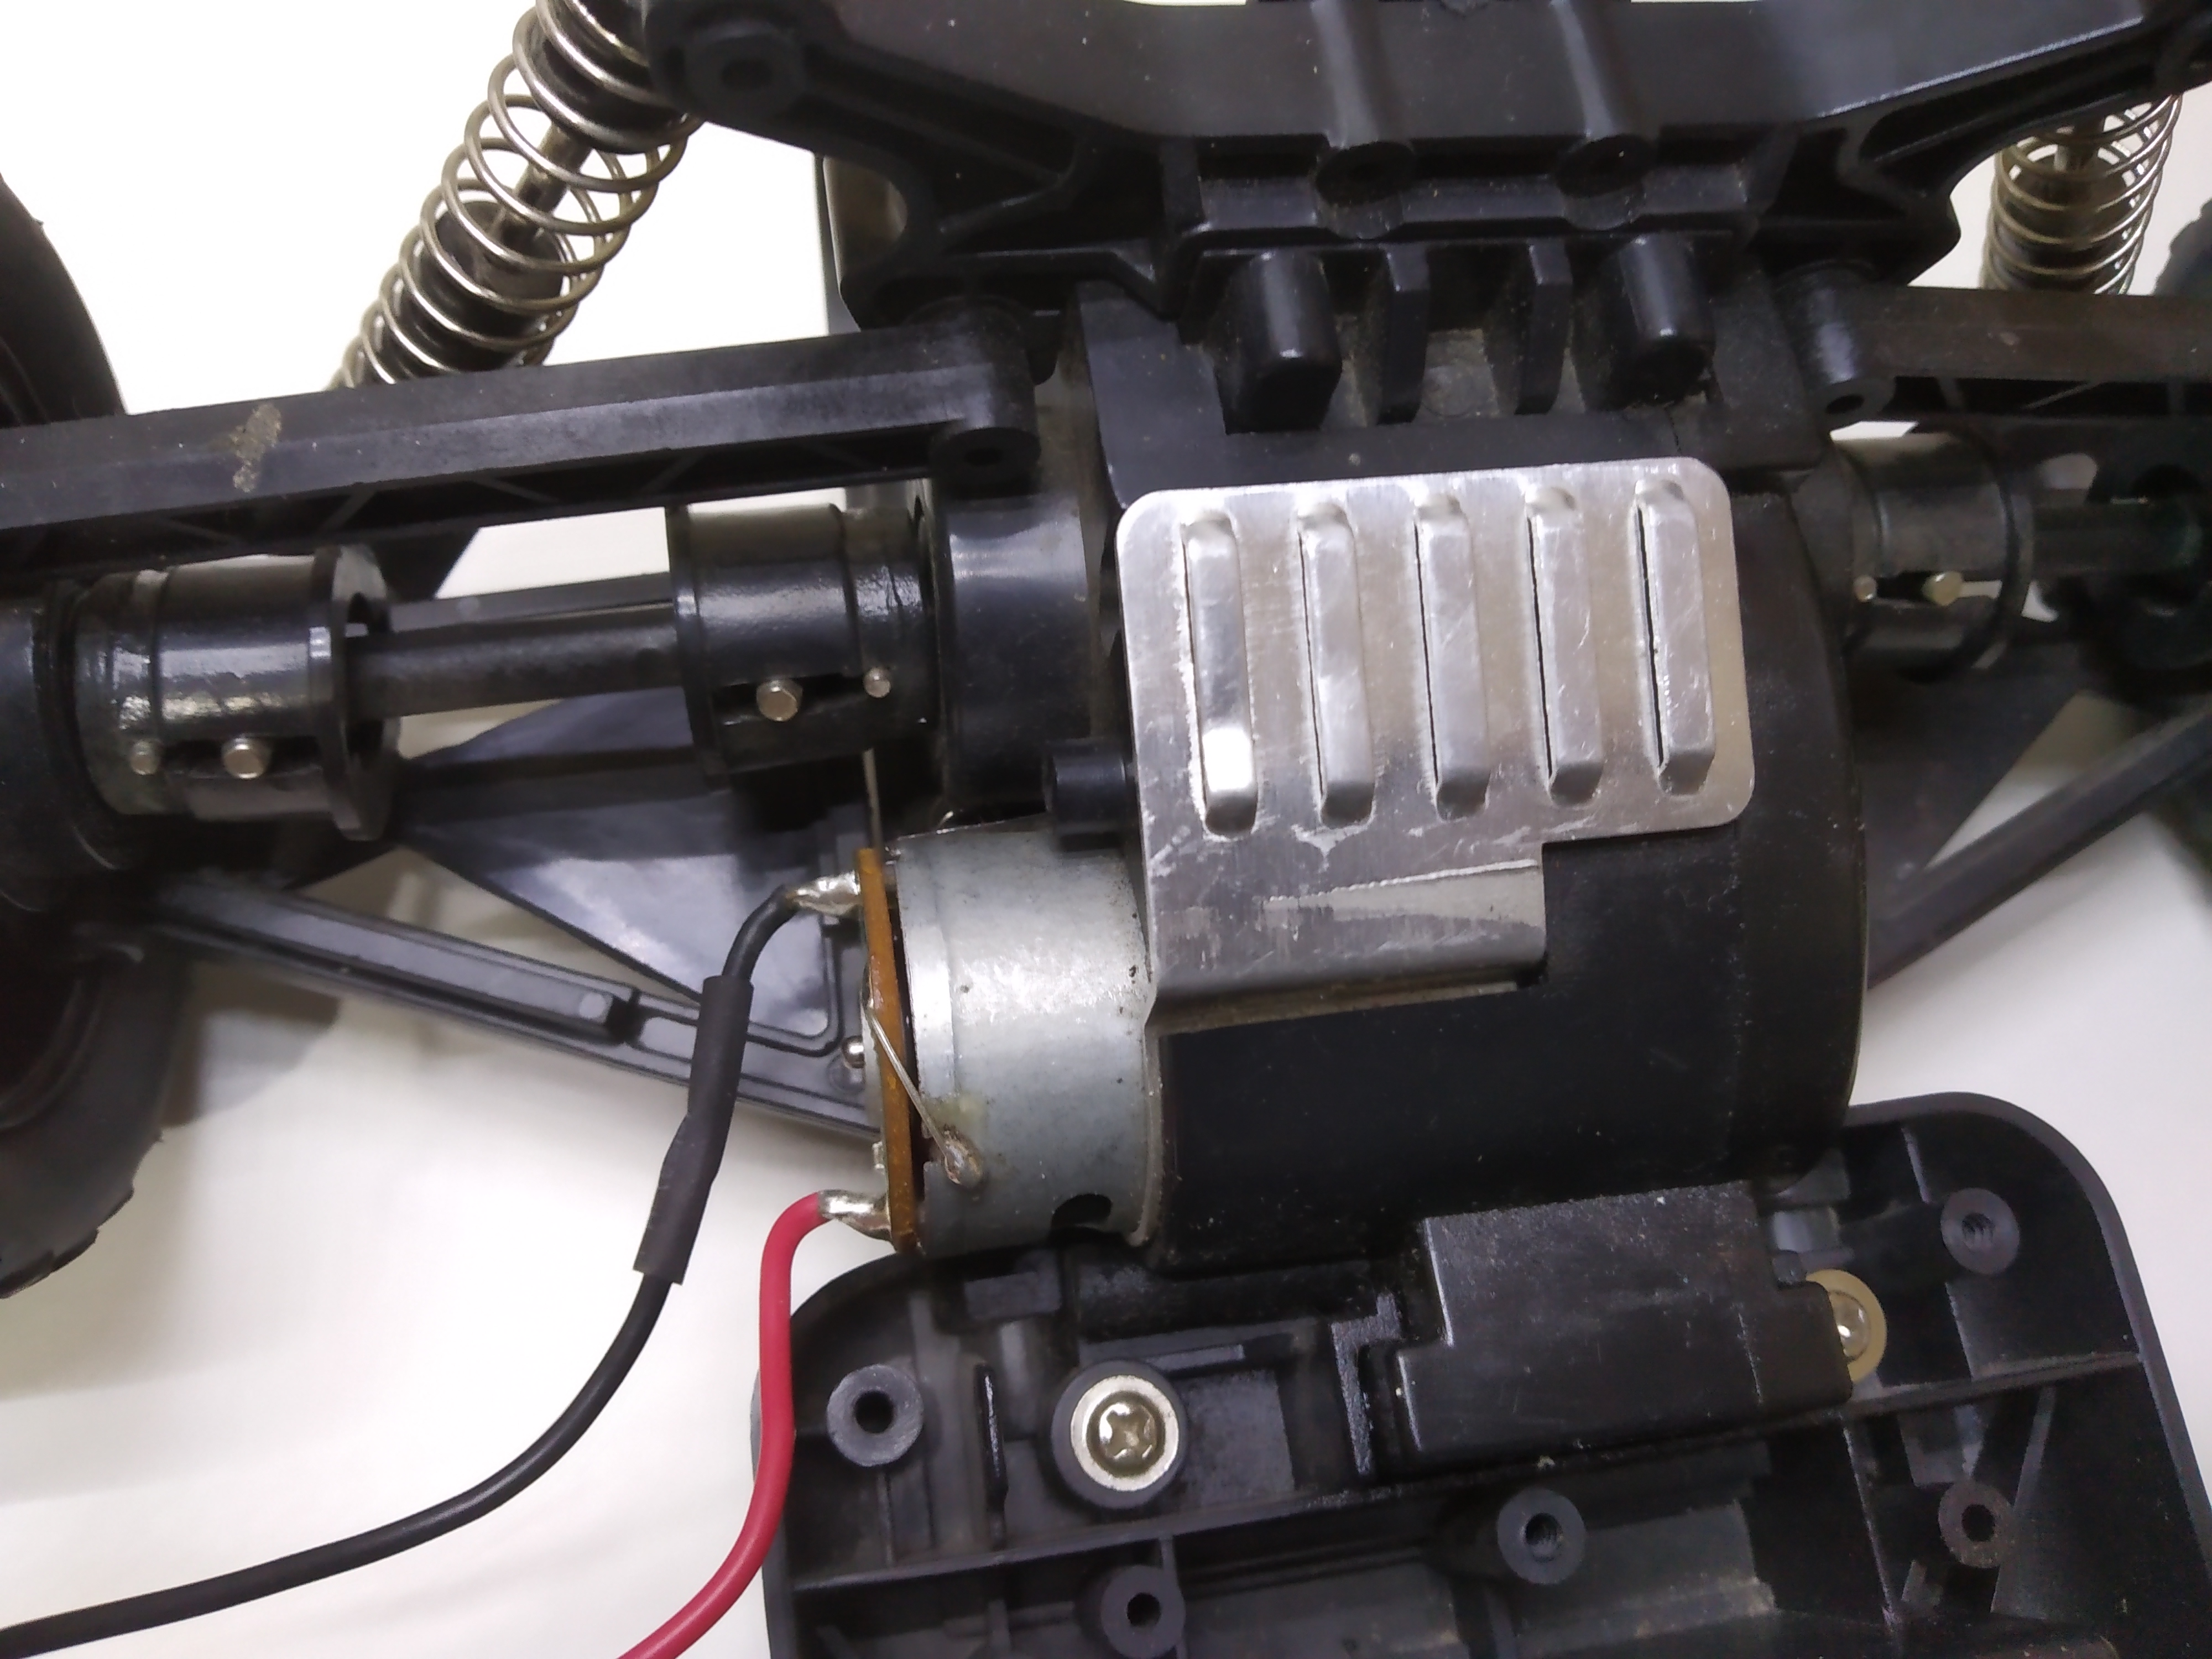
\includegraphics[width=0.55\textwidth]{img/dcmotor}
        \caption[Fotografía del motor DC de aceleración]{Fotografía del motor DC de aceleración. Fuente: Elaboración propia. }
        \label{fig:dcmotor}
    \end{figure}

        \subsubsection{Control de actuadores mediante ROS}
        Tal como se pudo especificar en la Sección(\ref{sec:mcu}) el microcontrolador elegido para la tarea tiene la capacidad de usar la 
        librería Rosserial que hace posible crear un nodo de ROS en el microcontrolador usando el puerto serial. En este sentido, 
        el control de motores se realiza de manera asíncrona con un tiempo de muestreo fijo. Se puede apreciar el algoritmo 
        implementado en el nodo de control en el Algoritmo(\ref{alg:nodomcu}).

        \begin{algorithm}
            \begin{algorithmic}[1]
            %\REQUIRE Complejo simplicial $K=\{\sigma_1, \dots, \sigma_n \}$ no vacío. \label{lin:lineaRara}
            %\ENSURE \TRUE si $K$ es contráctil y \FALSE en caso contrario.
            \STATE Conexión con el ros master
            \WHILE {No hay conexión}
            \STATE Intentar conexión
            \ENDWHILE
            
            \WHILE {Conectado con el ros master}
                \IF{Hay mensaje de control pendiente}
                    \STATE Calcular señal de control
                    \STATE Enviar comando a los actuadores
                \ENDIF
            \ENDWHILE
            \end{algorithmic}
            \caption{Algoritmo de control de actuadores}\label{alg:nodomcu}
        \end{algorithm}
        
        En este caso, el microcontrolador entra en un bucle que se ejecuta mientras exista conexión con el maestro. Dentro del 
        bucle, espera la llegada de algún mensaje de control para realizar un pequeño cálculo dependiendo a la calibración de 
        los mismos con el fin de enviar una señal de control adecuada para la actuación del vehículo.

        En la Figura(\ref{fig:joy_serial}) se puede apreciar el diagrama de comunicación entre los nodos de ros correspondientes con el nodo serial 
        y un control manual con un joystick.

        %%% figura del nodo rosserial

        \begin{figure}[!h] 
            \centering
            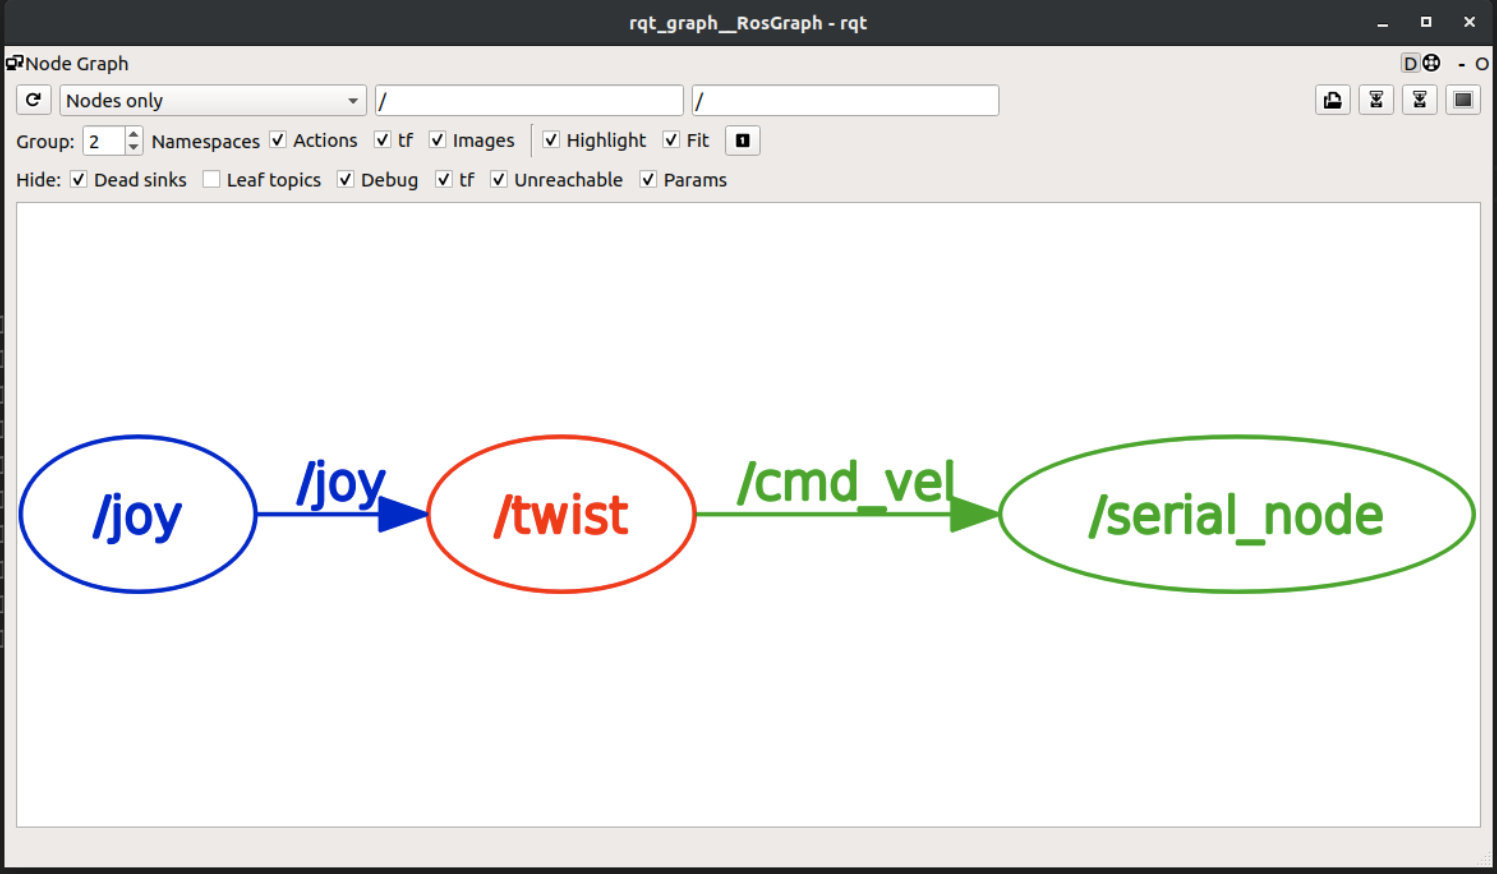
\includegraphics[width=0.55\textwidth]{img/joy_serial}
            \caption[Visualización del nodo serial]{Visualización del nodo serial. Fuente: Elaboración propia. }
            \label{fig:joy_serial}
        \end{figure}
        
        En el caso del control manual, existen tres nodos ejecutándose:
        \begin{itemize}
            \item \textbf{/joy} es el nodo que recupera los datos provenientes del joystick, botones presionados y valores de los potenciometros provenientes de los joysticks analógicos y los triggers. Este nodo publica mensajes de tipo \lstinline{joy} en el tópico \lstinline{/joy}.
            \item \textbf{/twist} es el nodo que convierte los datos de entrada del joystick en comandos de control de aceleración y dirección. Se suscribe al tópico \lstinline{/joy} y publica mensajes de tipo \lstinline{Twist} en el tópico \lstinline{/cmd_vel}.
            \item \textbf{/serial\_node} es el nodo que se comunica con el microcontrolador mediante el puerto serial. El nodo se suscribe a los mensajes publicados en el tópico \lstinline{/cmd_vel}.
        \end{itemize}

    \subsection{Módulo de la computadora de abordo}
    Mientras que el módulo de control de tiempo real se encarga de traducir los mensajes de control de ROS en señales de control 
    para aplicarse directamente a los actuadores por el microcontrolador a través de un controlador de potencia, la computadora 
    de abordo u OBC, se encarga se controlar todos los aspectos de \textit{alto nivel} del vehículo. Este módulo se compone de 
    una SBC corriendo un sistema operativo Linux con una distribución de ROS instalada en ella. La OBC será la responsable de 
    la comunicación con todos los nodos que interactúan con el vehículo, tanto  de los nodos que generan datos del entorno como 
    las imágenes provenientes de la cámara o sensores; como con nodos que consumen estos datos y los procesan de alguna manera, 
    como el nodo del piloto automático. 

    En la Figura(\ref{fig:obc}) se puede apreciar la OBC y en la Figura(\ref{fig:carro}) el prototipo con la OBC incorporada al mismo. Cabe resaltar que por sus características, tanto 
    la OBC, como el módulo de control de tiempo real pueden alimentarse por una batería a bordo del vehículo. A su vez, la comunicación 
    inalámbrica de la OBC permite que el vehículo pueda funcionar sin la necesidad de un solo cable ya sea de alimentación de energía 
    o comunicación.

    \begin{figure}[!h] 
        \centering
        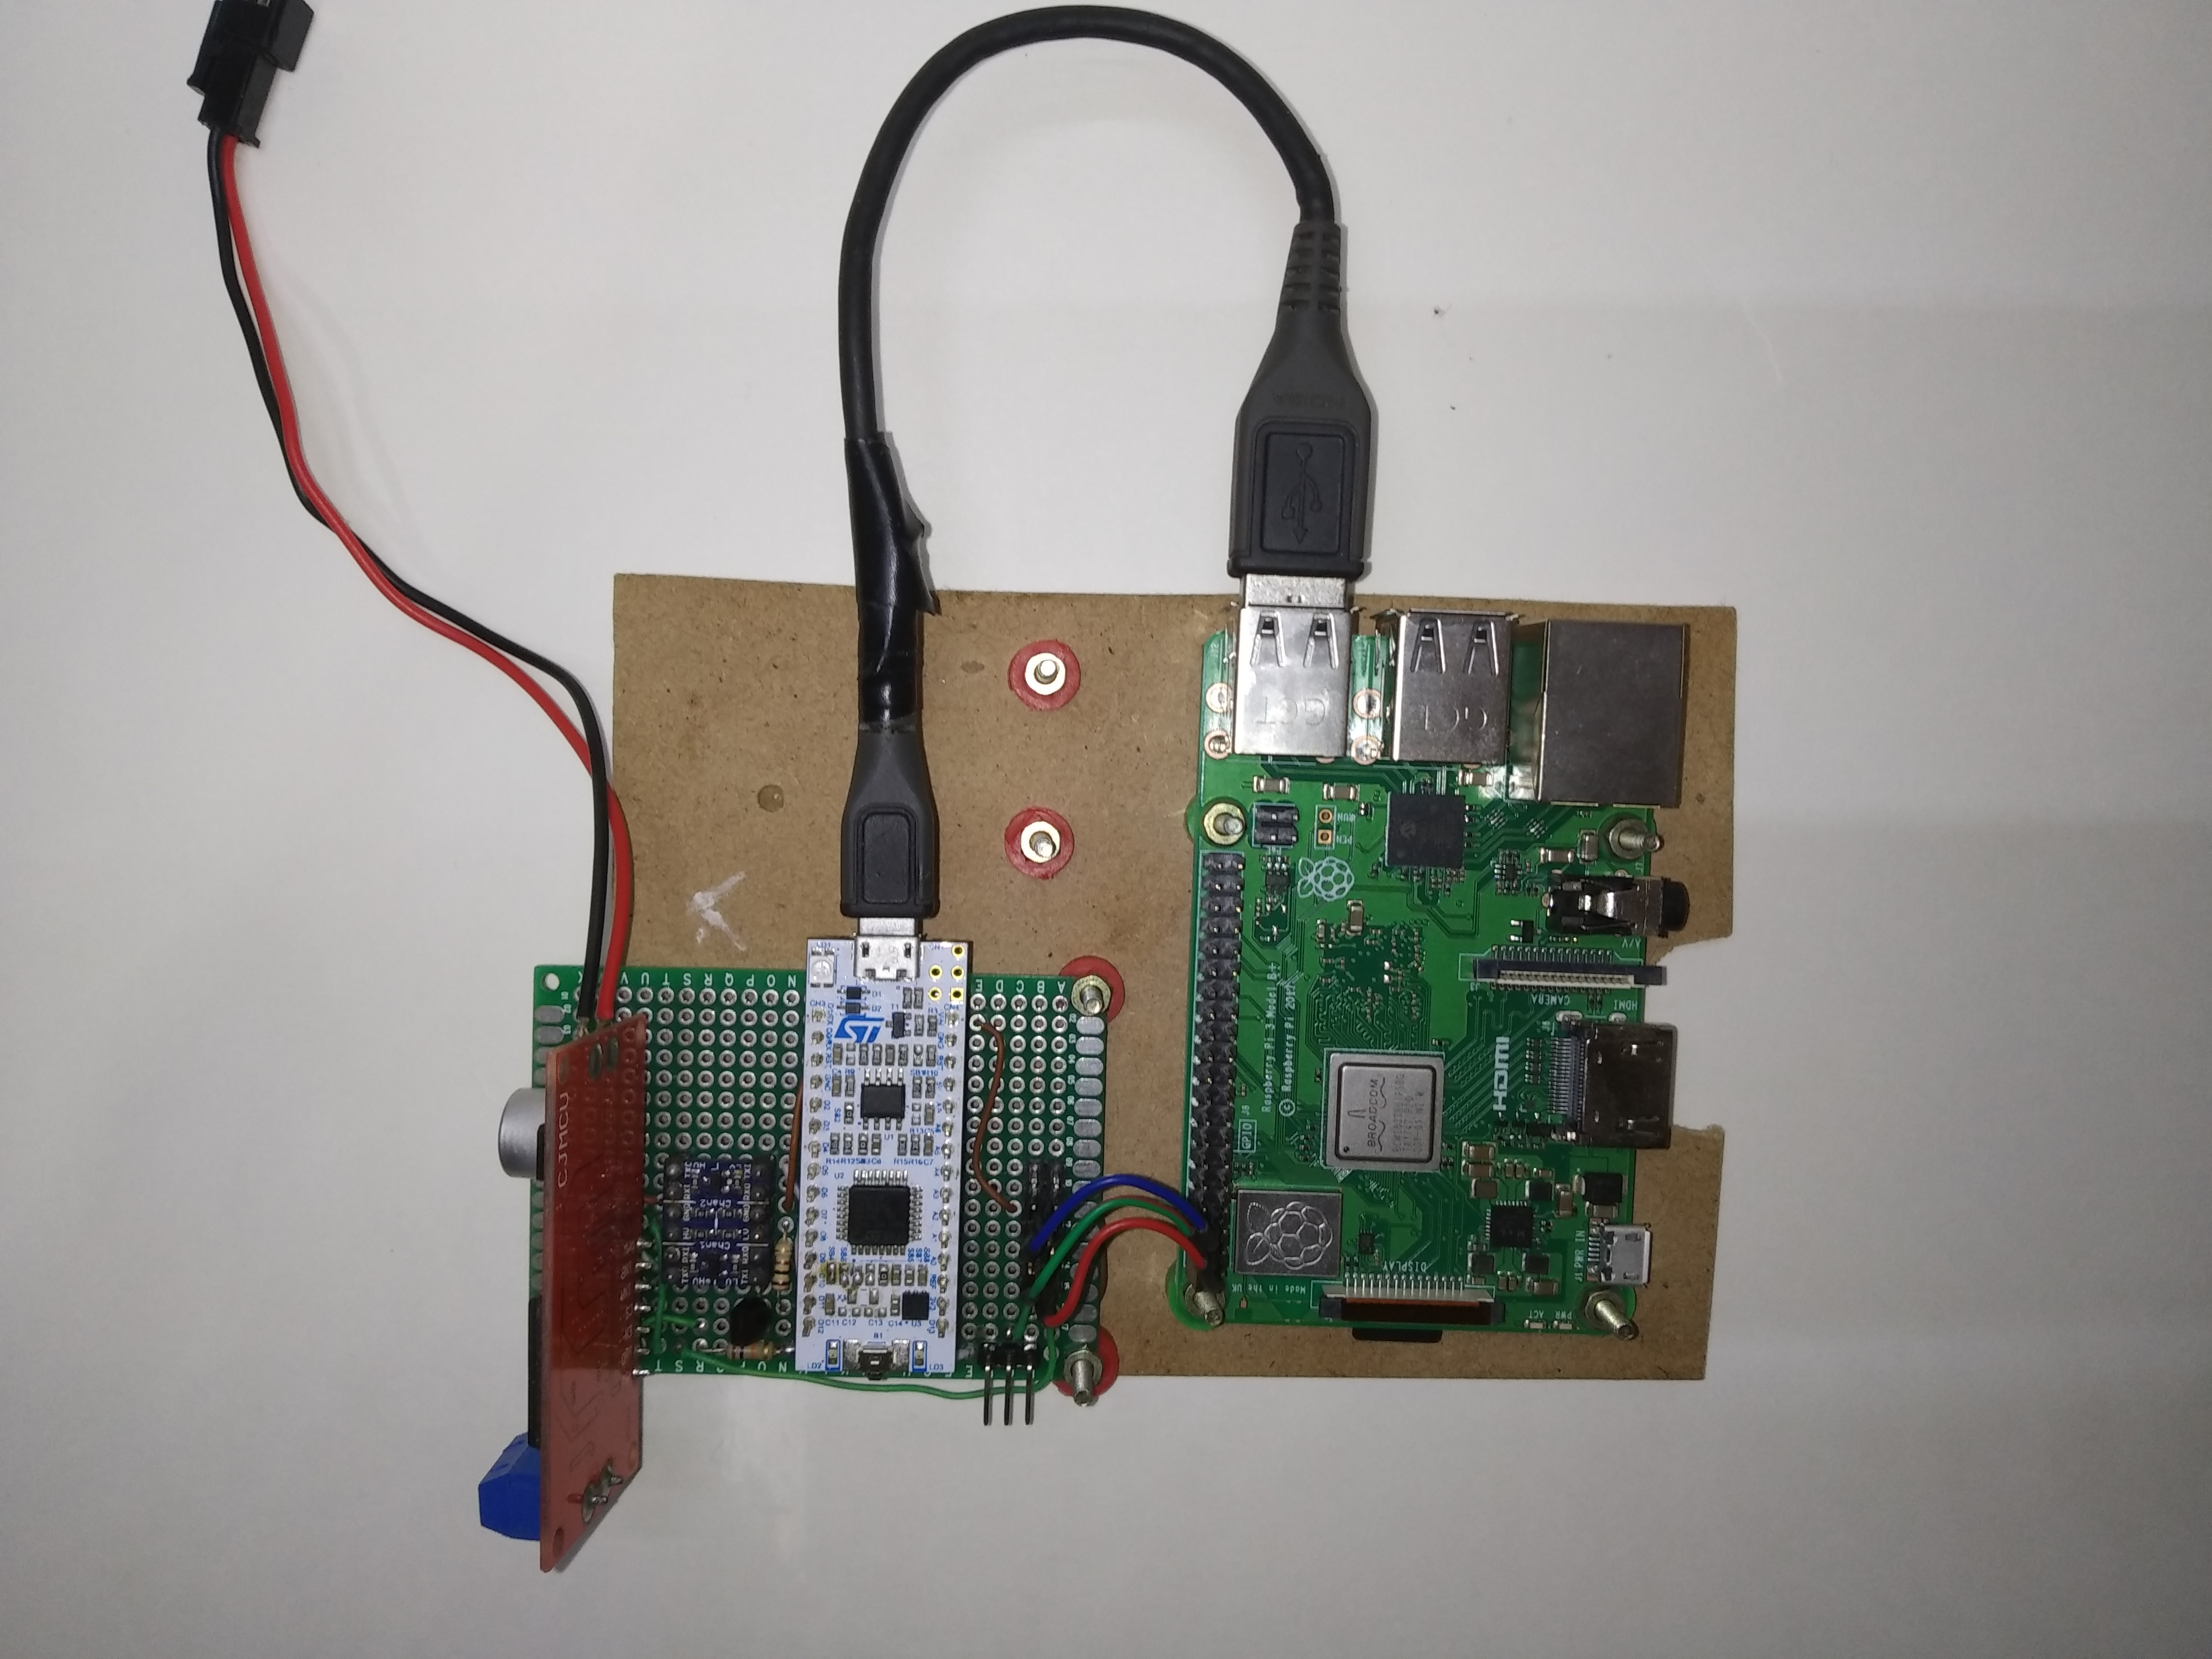
\includegraphics[width=0.55\textwidth]{img/obc}
        \caption[Fotografía de la OBC]{Fotografía de la OBC. Fuente: Elaboración propia. }
        \label{fig:obc}
    \end{figure}

    \begin{figure}[!h] 
        \centering
        \includegraphics[width=0.65\textwidth]{img/carro}
        \caption[Fotografía del prototipo]{Fotografía del prototipo. Fuente: Elaboración propia. }
        \label{fig:carro}
    \end{figure}


    \subsubsection{Esquema de comunicación en la OBC}
    La OBC corre el maestro de ROS, que es el que arbitra toda la comunicación en el sistema y, junto con eso, también se encarga 
    de ejecutar varios nodos correspondientes con los sensores y el control. Por su parte, el esquema de comunicación entre dichos nodos, se puede apreciar en 
    la Figura(\ref{fig:nodosobc}).

    
    \begin{figure}[!h] 
        \centering
        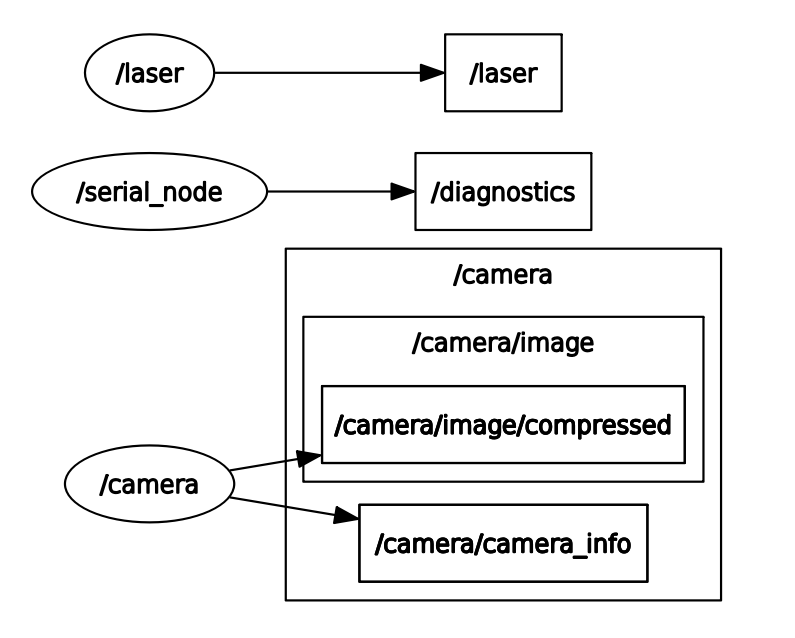
\includegraphics[width=0.55\textwidth]{img/nodosobc}
        \caption[Interacción de los nodos en la OBC]{Interacción de los nodos en la OBC. Fuente: Elaboración propia. }
        \label{fig:nodosobc}
    \end{figure}
    
    La lista detallada de los nodos que corren en la OBC se puede observar en la Tabla(\ref{tbl:nodosobc}). Se puede rescatar la naturaleza modular 
    del sistema usando el \textit{middleware} de ROS dado que cada nodo se suscribe (si corresponde) a un tópico del cual obtendrá
    mensajes con la información necesaria, o publica mensajes producto de algún cálculo o proceso de adquisición.

    % Please add the following required packages to your document preamble:
    % \usepackage{booktabs}
    % \usepackage{multirow}
    % \usepackage{graphicx}
    \begin{table}[]
        \centering
        \resizebox{\textwidth}{!}{%
        \begin{tabular}{@{}|c|c|c|c|c|@{}}
        \toprule
        \multirow{2}{*}{\textbf{Nodo}} & \multicolumn{2}{c|}{\textbf{Subscribe}} & \multicolumn{2}{c|}{\textbf{Publica}}                                                                                                                                                    \\ \cmidrule(l){2-5} 
                                    & \textbf{Tópicos} & \textbf{Mensajes}    & \textbf{Tópicos}                                                                        & \textbf{Mensajes}                                                                              \\ \midrule
        /serial\_node                  & /cmd\_vel        & geometry\_msgs/Twist & /diagnostics                                                                            & diagnostics\_msgs/DiagnosticArray                                                              \\ \midrule
        /laser                         & -                & -                    & /laser                                                                                  & sensor\_msgs/Range                                                                             \\ \midrule
        /camera                        & -                & -                    & \begin{tabular}[c]{@{}c@{}}/camera/image/compressed\\ /camera/camera\_info\end{tabular} & \begin{tabular}[c]{@{}c@{}}sensor\_msgs/CompressedImage\\ sensor\_msgs/CameraInfo\end{tabular} \\ \bottomrule
        \end{tabular}%
        }
        \caption[Nodos de interfaz con los actuadores y sensores]{Nodos de interfaz con los actuadores y sensores. Fuente: Elaboración propia}
        \label{tbl:nodosobc}
        \end{table}
    
    Dado que ROS permite el desarrollo de sistemas distribuidos, existen otros nodos que se ejecutan en la estación de trabajo y 
    se comunican con el maestro, corriendo en la OBC, a través de Wifi mediante una conexión TCP. La implementación de la comunicación 
    en la red está implementada en el \textit{middleware} de ROS y este proyecto no se concentra en los detalles de la misma.
    
    \subsubsection{Nodo /serial\_node}
    Este nodo se encarga de establecer la conexión con el módulo de potencia en tiempo real a través de un puerto serial. El 
    microcontrolador es capaz de enviar y recibir mensajes como si se tratara de un nodo común de ROS. El nodo serial es parte 
    del paquete \lstinline{rosserial}\cite{ferguson} y publica información de conexión en un tópico de diagnóstico, este tópico es 
    útil en la depuración y cuando existen problemas en la comunicación serial con el microcontrolador.

    \subsubsection{Nodo /laser}
    Este nodo se encarga de publicar mensajes del tipo \lstinline{sensor_msgs/Range} con información sobre el sensor de proximidad 
    que se encuentra en frente del vehículo. Se establece la comunicación mediante el protocolo I2C \footnote{I2C: Circuito inter-integrado (I2C, del inglés Inter-Integrated Circuit) es un bus serie de datos para la comunicación entre diferentes partes de un circuito, por ejemplo, entre un controlador y circuitos periféricos integrados.}
    con el sensor VL53L0X (Sección(\ref{sec:laser})) y se adecúan los datos para ser publicados en el tópico \lstinline{/laser}.

    \subsubsection{Nodo /camera}
    Este nodo realiza la conexión con la cámara conectada a la OBC, la Raspberry Pi Camera Module V2 (Sección(\ref{sec:raspicam})) 
    y publica las imágenes en formato compreso JPEG \footnote{JPEG: Estándar de compresión y codificación de archivos e imágenes.}
    para utilizar menos ancho de banda. Las imágenes se publican en el tópico \lstinline{/camera/image/compressed}. El nodo 
    es parte del paquete \lstinline{raspicam_node} \cite{agrawalgramlich2018}.


\section{Subsistema de Adquisición de Datos y Entrenamiento}\label{sec:daq}

Una vez establecida la plataforma de trabajo en el Subsistema de Control y Actuación se procede a detallar el diseño del 
Subsistema de Adquisición de Datos y Entrenamiento que se encarga principalmente de brindar una forma adecuada de sincronizar 
y almacenar los datos necesarios para el entrenamiento de la red neuronal así como también de brindar las herramientas necesarias 
para el entrenamiento en sí. Este subsistema cuenta con vários módulos funcionales que interactúan entre sí como se pudo apreciar 
en la Sección(\ref{sec:esqdaq}). 

    \subsection{Módulo de adquisición de datos y operación manual}
    Como se ha podido establecer en la Sección(\ref{sec:redesneuronales}) referida al aprendizaje automático. Para que un algoritmo de aprendizaje pueda 
    entrenarse de manera efectiva, es necesario contar con un conjunto de datos sobre el cual se realizará el mismo. Este conjunto 
    de datos o \textit{dataset} necesita estar almacenado de manera adecuada con el formato y las características necesarias para 
    un entrenamiento efectivo.
    
    % foto del joystick
    \begin{figure}[!h] 
        \centering
        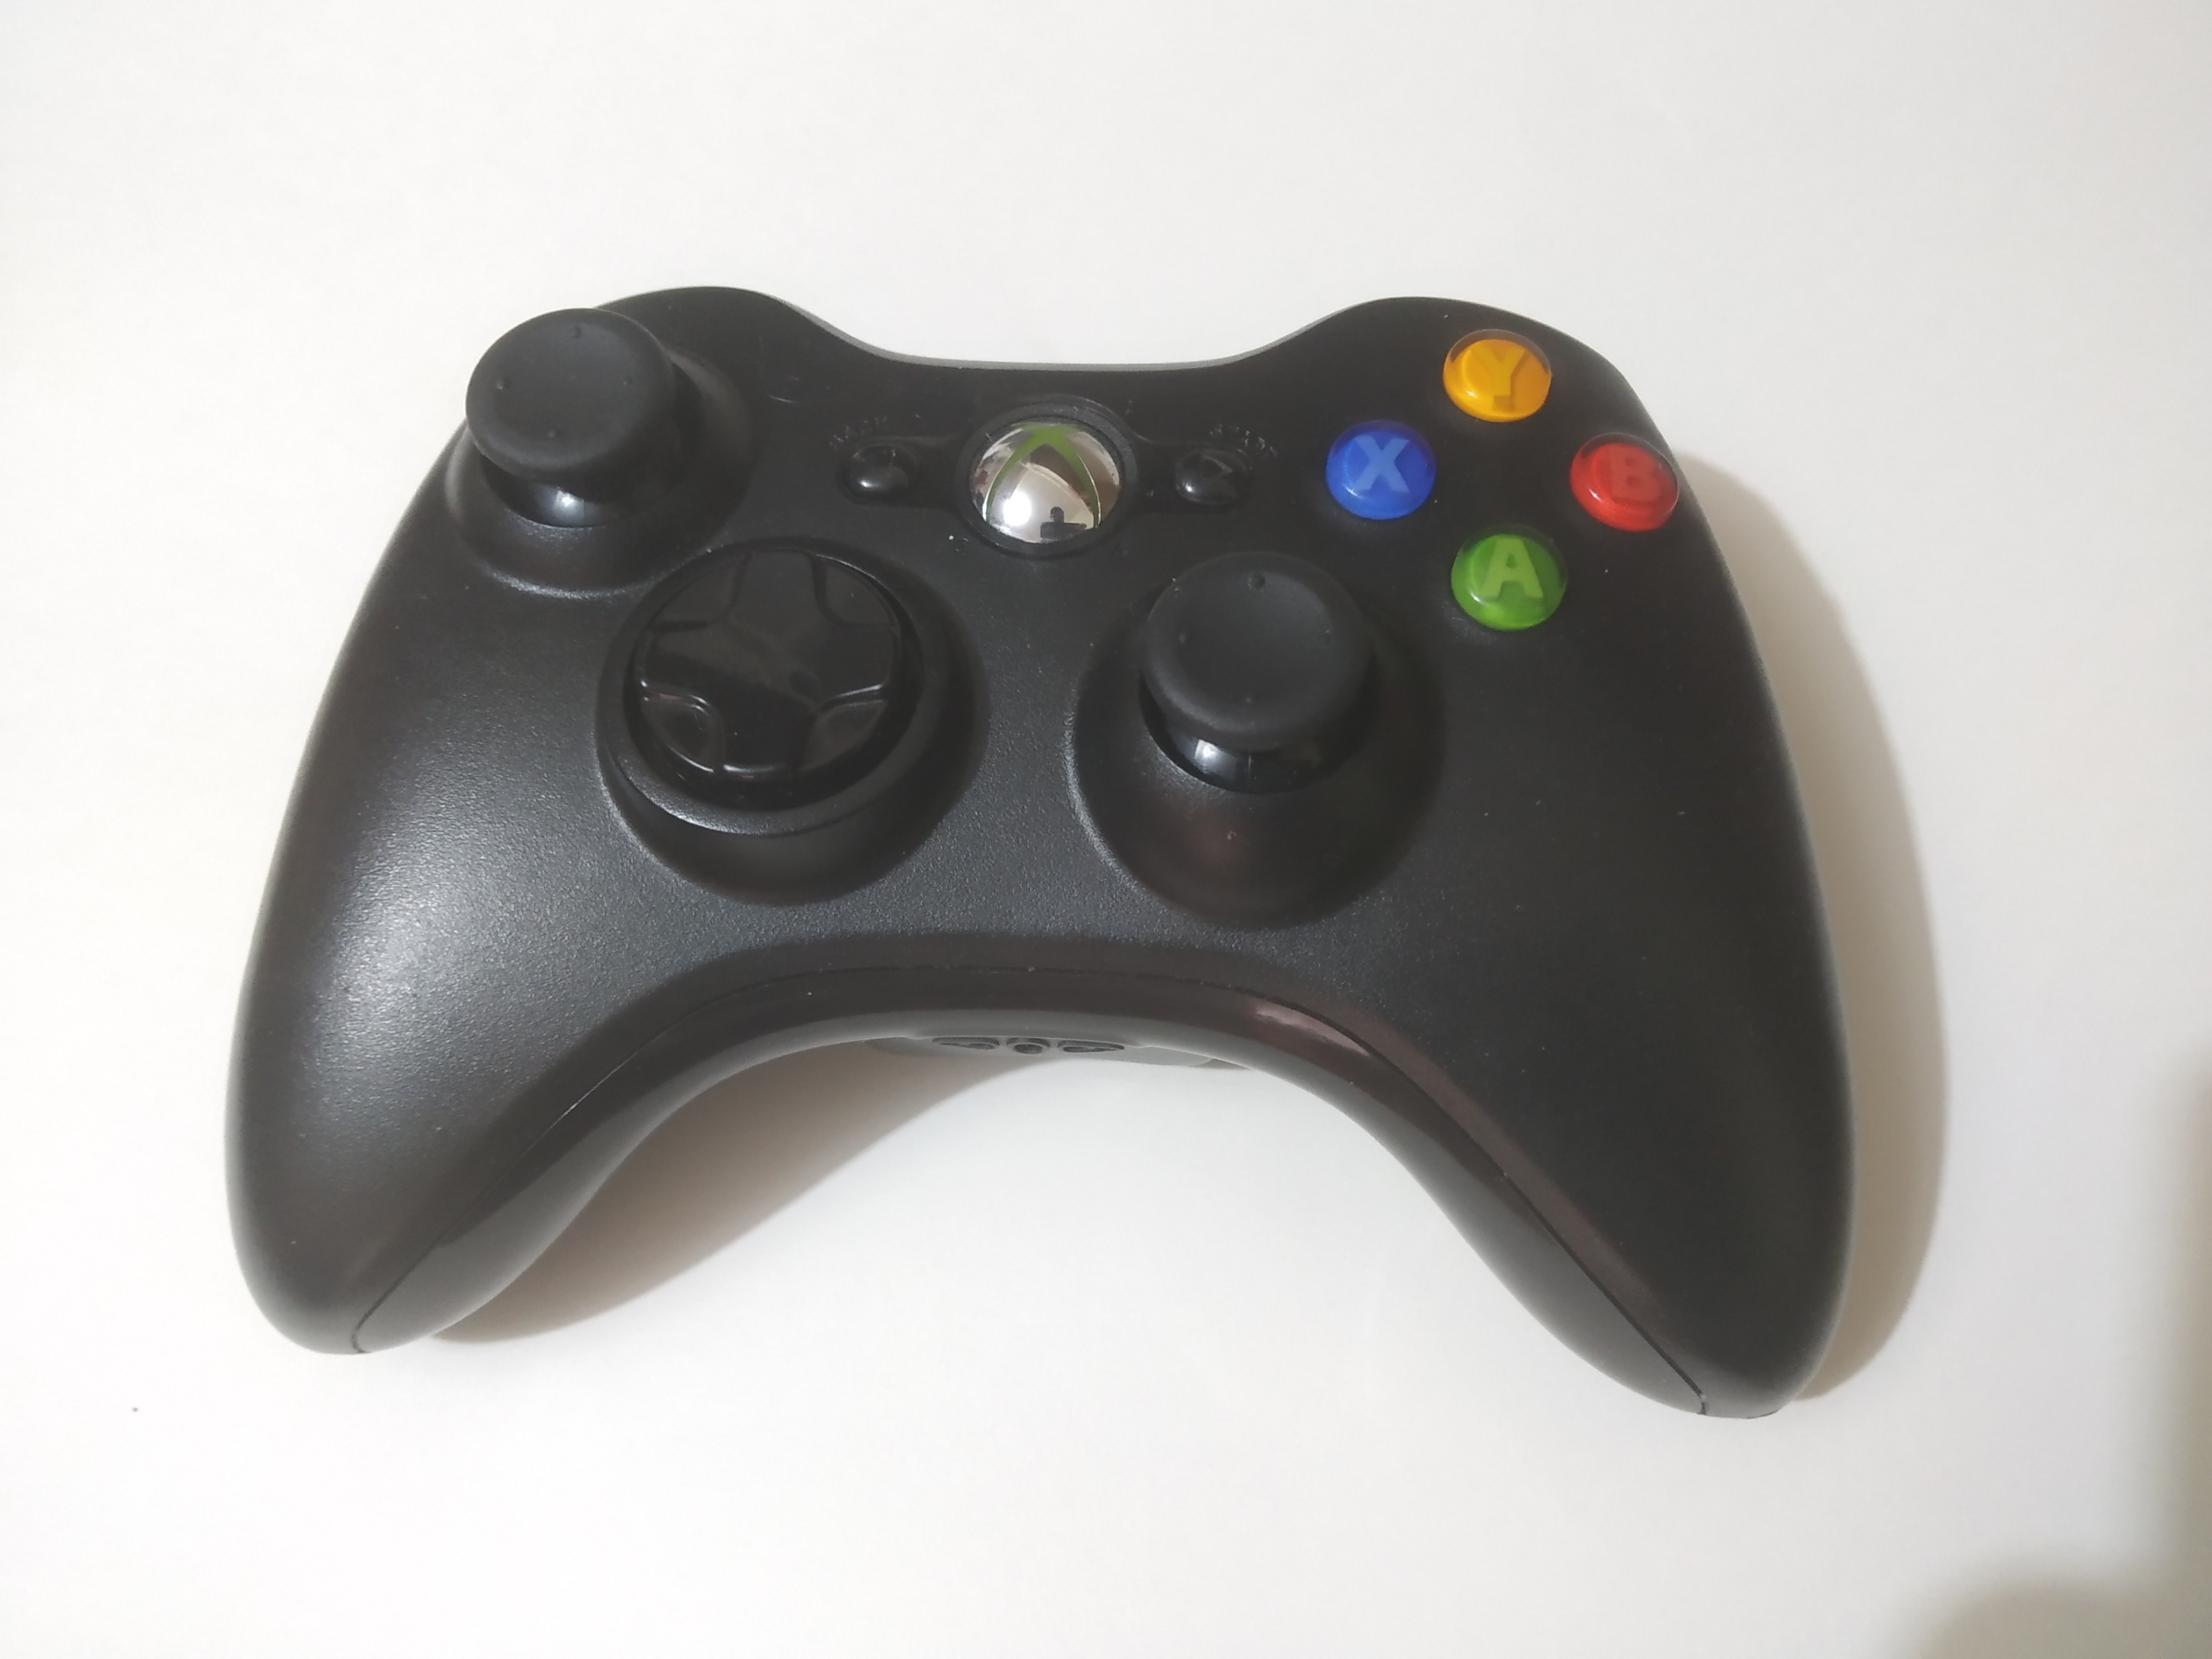
\includegraphics[width=0.55\textwidth]{img/joystick}
        \caption[Fotografía del mando inalámbrico de Xbox 360]{Fotografía del mando inalámbrico de Xbox 360. Fuente: Elaboración propia. }
        \label{fig:joystick}
    \end{figure}

    El módulo cuenta con un nodo que se suscribe a los mensajes provenientes tanto de la cámara como del control manual con el 
    joystick (Figura(\ref{fig:joystick})). Luego, se realiza una sincronización para que se pueda generar un par entrada - salida 
    adecuado y luego se procede a almacenar el mismo. En la Figura(\ref{fig:nodosdaq}) se puede apreciar el grafo de comunicación de los 
    nodos concernientes a este módulo.


    % diagrama del modulo
    
    \begin{figure}[!h] 
        \centering
        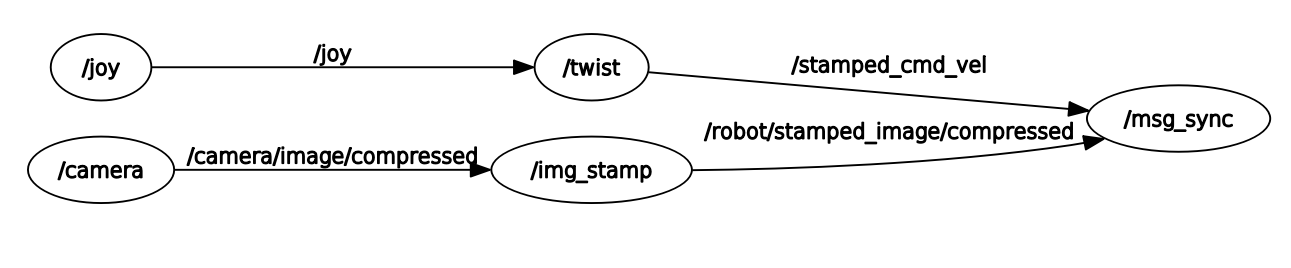
\includegraphics[width=0.95\textwidth]{img/nodosdaq}
        \caption[Esquema de nodos para la adquisición de datos]{Esquema de nodos para la adquisición de datos. Fuente: Elaboración propia. }
        \label{fig:nodosdaq}
    \end{figure}

    El nodo \lstinline{/msg_sync} se encarga de recuperar los mensajes de la cámara y del joystick y sincronizarlos para luego 
    guardar la imagen en un archivo \lstinline{.bmp} y su correspondiente información en el archivo \lstinline{target.csv}. 
    Se puede observar el procedimiento en el Algoritmo(\ref{alg:msgsync}).

    \begin{algorithm}
        \begin{algorithmic}[1]
        %\REQUIRE Complejo simplicial $K=\{\sigma_1, \dots, \sigma_n \}$ no vacío. \label{lin:lineaRara}
        %\ENSURE \TRUE si $K$ es contráctil y \FALSE en caso contrario.
        \STATE Subscripción a \lstinline{/stamped_cmd_vel}
        \STATE Subscripción a \lstinline{/robot/stamped_image/compressed}
        \STATE Registrar callback
        
        \WHILE {Conectado con el ros master}
            \LOOP
            \IF{Llegan mensajes sincronizados}
                \STATE Decodificar imagen
                \STATE Redimensionar imagen
                \STATE Guardar archivo
                \STATE Generar registro con datos de entrada/salida
                \STATE Actualizar registro en el archivo \lstinline{target.csv}
            \ENDIF
            \ENDLOOP
        \ENDWHILE
        \end{algorithmic}
        \caption{Algoritmo de sincronización de mensajes y almacenamiento de datos.}\label{alg:msgsync}
    \end{algorithm}

    El \textit{dataset} se compone de un conjunto de imágenes en formato \lstinline{PNG} junto con un archivo \lstinline{CSV} que 
    contiene las columnas detalladas en la Tabla(\ref{tbl:columns}). En la tabla se almacenan tanto los datos de aceleración y dirección como el 
    nombre del archivo de la imagen correspondiente con la misma. Los registros se almacenan en el mismo orden en el que fueron 
    capturados, no obstante, para la tarea de regresión definida en este proyecto, la dependencia temporal entre las muestras 
    no es importante. 

        % Please add the following required packages to your document preamble:
    % \usepackage{booktabs}
    % \usepackage{graphicx}
    \begin{table}[!h]
        \centering
        \resizebox{0.55\textwidth}{!}{%
        \begin{tabular}{@{}|c|c|c|@{}}
        \toprule
        \textbf{Columna} & \textbf{Descripción} & \textbf{Tipo de dato} \\ \midrule
        id & \begin{tabular}[c]{@{}c@{}}Número de identificación\\ único para cada muestra del \\ dataset.\end{tabular} & Int32 \\ \midrule
        angular & \begin{tabular}[c]{@{}c@{}}Valor del comando de \\ dirección proveniente \\ del Joystick \\ 1: completamente a la izquierda\\ -1: completamente a la derecha\\ 0: adelante\end{tabular} & Float32 \\ \midrule
        imgpath & \begin{tabular}[c]{@{}c@{}}Nombre del archivo de la \\ imagen correspondiente con \\ el id actual\end{tabular} & String \\ \midrule
        linear & \begin{tabular}[c]{@{}c@{}}Valor del comando de \\ aceleración proveniente \\ del Joystick \\ 1: aceleración máxima adelante\\ -1: aceleración máxima atrás\\ 0: detenido\end{tabular} & Float32 \\ \midrule
        target & \begin{tabular}[c]{@{}c@{}}Par de valores correspondientes\\  con los valores angular y linear.\end{tabular} & Array \\ \bottomrule
        \end{tabular}%
        }
        \caption{Columnas de la tabla del conjunto de datos generado}
        \label{tbl:columns}
    \end{table}
    
        \subsubsection{Sesiones de entrenamiento}
        La manera de adquirir el conjunto de datos es mediante las denominadas \textit{Sesiones de Entrenamiento o Grabación de Comportamiento}.
        Estas sesiones corresponden con periodos de tiempo en el cual se recuperan datos de manera constante. La cantidad de registros 
        o muestras recuperadas depende tanto de la resolución temporal de la generación de imágenes y comandos de control sincronizados 
        así como también de la duración de la sesión en sí. Cada sesión de entrenamiento puede generar un \textit{dataset} distinto 
        que se puede combinar con otros \textit{datasets} o tomarse de manera independiente. 

        Es importante tomar en cuenta que mientras más sesiones se realicen y más variadas en condiciones ambientales sean las mismas, 
        más robusto será el algoritmo entrenado y mejor será su generalización. Sin embargo, esta capacidad de generalización estará 
        limitada por la arquitectura y la cantidad de parámetros disponibles para generar representaciones internas del proceso. 

        En el presente proyecto, se han realizado sesiones de entrenamiento con un clima parcialmente nublado con buena iluminación 
        ambiental, de manera que se pueda distinguir la pista del piso (Figura(\ref{fig:fotosejemplo})).

        %% foto de ejemplo
        \begin{figure}[!h] 
            \centering
            \includegraphics[width=0.75\textwidth]{img/fotosejemplo}
            \caption[Imágenes capturadas por la cámara en una sesión de entrenamiento]{Imágenes capturadas por la cámara en una sesión de entrenamiento. Fuente: Elaboración propia. }

            \label{fig:fotosejemplo}
        \end{figure}

    \subsection{Módulo de aumentación de datos}\label{sec:aumentacion}
    Las redes neuronal profundas tienen la impresionante capacidad de aprender representaciones internas útiles de manera automática 
    usando el algoritmo de la retropropagación, pero esta capacidad solamente resalta cuando se cuenta con un conjunto de datos 
    de un tamaño considerable, es decir, que se necesitan muchas muestras para que el entrenamiento de una red neuronal profunda 
    sea exitosa y pueda mostrar resultados favorables. 
    
    Por su parte, la recuperación de datos es un proceso costoso en tiempo y recursos, por lo que no se puede invertir demasiado 
    tiempo solamente recuperando muestras. De hecho, se ha establecido que el proceso de la generación de un \textit{dataset} efectivo 
    es el más complicado en un sistema de aprendizaje automático. Por tanto, es importante poder aprovechar al máximo los datos 
    obtenidos en una sesión de entrenamiento.

    Es por este motivo que se ha decidido incluir una etapa de aumentación de datos que se compone de una serie de transformaciones 
    de las imágenes originales del \textit{dataset} para poder incrementar la cantidad de muestras sobre la cual se realice el 
    entrenamiento de la red de manera sintética. En la Tabla(\ref{tbl:transf}) se puede apreciar las transformaciones usadas.
    
    % tabla de transformaciones 
    % Please add the following required packages to your document preamble:
    % \usepackage{booktabs}
    % \usepackage{graphicx}
    \begin{table}[!h]
        \centering
        \resizebox{0.65\textwidth}{!}{%
        \begin{tabular}{@{}|c|c|@{}}
        \toprule
        \textbf{Transformación} & \textbf{Descripción}                                                                                                      \\ \midrule
        Rotación                & \begin{tabular}[c]{@{}c@{}}Se rota la imagen un ángulo \\ aleatorio entre -20 y 20 grados.\end{tabular}                   \\ \midrule
        Desplazamiento Vertical & \begin{tabular}[c]{@{}c@{}}Se desplaza la imagen de forma \\ vertical un valor aleatorio entre \\ 0 y 20 \%.\end{tabular} \\ \midrule
        Espejo Horizontal       & \begin{tabular}[c]{@{}c@{}}Se invierte la imagen \\ hotizontalmente de forma aleatoria.\end{tabular}                      \\ \bottomrule
        \end{tabular}%
        }
        \caption{Transformaciones realizadas en la aumentación de datos. Fuente: Elaboración propia.}
    \label{tbl:transf}
    \end{table}

    Este módulo no solamente cuenta con ciertas transformaciones disponibles para aumentar los datos existentes en el \textit{dataset}
    si no también cuenta con la funcion de poder eliminar registros con un valor de dirección nulo si es que fuera necesario. La utilidad
    de esta funcionalidad se puede apreciar en la etapa de entrenamiento en la Sección(\ref{sec:training}). El algoritmo para 
    la aumentación de datos se puede apreciar en el Algoritmo(\ref{alg:msgsync}).

    \begin{algorithm}
        \begin{algorithmic}[1]
        %\REQUIRE Complejo simplicial $K=\{\sigma_1, \dots, \sigma_n \}$ no vacío. \label{lin:lineaRara}
        %\ENSURE \TRUE si $K$ es contráctil y \FALSE en caso contrario.
        \STATE Carga del dataset
        \STATE Configuración de los parámetros de transformación
        \STATE Iniciar generador de pares $(imagen,target)$
        \FOR {imagen}
            \STATE $img_{aux} = imagen$
            \IF{$abs(target) > 0.09$}       
                \STATE $hTarget = -target$  
                \STATE $hImg = flipHorizontal(img_{aux})$
                \STATE Guardar $(hImg,hTarget)$
                \STATE $nImg = shiftVertical(img_{aux})$
                \STATE $nImg = rotacion(nImg)$
                \STATE Guardar $(hImg,target)$
            \ENDIF
        \ENDFOR
        
        \end{algorithmic}
        \caption{Algoritmo del módulo de aumentación de datos.}\label{alg:msgsync}
    \end{algorithm}

    En el caso de la transformación de espejo horizontal, se debe invertir también la salida o \textit{target} de la imagen 
    para que corresponda con el espejo, es decir, que si para una imagen $img$ el $target = 0.67$ para su transformación $hImg = flipHorizontal(img)$ 
    se debe crear un nuevo $hTarget = -target = -0.67$. 

    Para las transformaciones de desplazamiento vertical y rotación, se mantiene el $target$ original de la imagen pues no se 
    afecta la naturaleza de la imagen de manera sustancial.


    \subsection{Módulo de generación de datos de entrenamiento}

    Una de las desventajas de las redes neuronales convolucionales para el procesamiento de imágenes es que las imágenes 
    ocupan bastante espacio en memoria y cargar todo el conjunto de datos de entrenamiento en la memoria RAM es usualmente 
    imposible o demasiado costoso. Es por eso que se necesita una forma de cargar las imágenes en la memoria de forma 
    fraccionada, de manera que los requisitos de memoria sean manejables por la estación de trabajo. 

    El módulo de generación de datos de entrenamiento se ha desarrollado con la finalidad de poder generar \textit{mini batches} 
    o conjuntos pequeños de datos para el entrenamiento de la red neuronal convolucional. El algoritmo de la generación se 
    detalla en el Algoritmo(\ref{alg:datagen}).

    \begin{algorithm}
        \begin{algorithmic}[1]
        \REQUIRE Tabla de datos, tamaño del mini-batch
        \STATE Reordenar el dataset aleatoriamente
        %\ENSURE \TRUE si $K$ es contráctil y \FALSE en caso contrario.
        \FOR {mini-batch}
            \STATE $X = [\dots]$
            \STATE $Y = [\dots]$
            \FOR {par$(imagen,target)$}
                \STATE Cargar $imagen$ desde el disco 
                \STATE Agregar $imagen$ a $X$
                \STATE Agregar $target$ a $Y$
            \ENDFOR
            \STATE Enviar $(X,Y)$
        \ENDFOR
        
        \end{algorithmic}
        \caption{Algoritmo del módulo de generación de datos.}\label{alg:datagen}
    \end{algorithm}

    Como se puede observar, para cada mini-batch generado se crean dos listas $X$ y $Y$ que contendrán los datos de 
    las imágenes y los targets. De esta manera ya no se necesita cargat todo el \textit{dataset} en la memoria ram pues se 
    cargarán solamente las imágenes del disco correspodiente a cada mini-batch.

    Este módulo es capaz de generar \textit{mini batches} de manera parametrizada de acuerdo a la necesidad de cada sesión de 
    entrenamiento.

    \subsection{Módulo de Entrenamiento}
    Una vez se tienen las herramientas para la correcta generación y aumentación de datos del conjunto de datos de entrenamiento 
    se necesita una herramienta para ejecutar el entrenamiento de la red neuronal convolucional en sí. El módulo de entrenamiento 
    se compone de un programa que ejecuta las siguientes tareas:

    \begin{itemize}
        \item Carga del dataset y el modelo de red neuronal.
        \item Definición de hiperparámetros.
        \item Ejecución, monitoreo y control del proceso de entrenamiento en línea. 
        \item Salvaguarda de los parámetros del modelo entrenado.
        \item Generación de reportes del proceso de entrenamiento.
    \end{itemize}

    En el Algoritmo(\ref{alg:training}) se puede apreciar el proceso detallado de entrenamiento de la red de acuerdo a parametrización definida 
    por el usuario. 
    
    % algoritmo del entrenamiento
    \begin{algorithm}
        \begin{algorithmic}[1]
        \REQUIRE Conjunto de datos, modelo de la red neuronal
        \STATE Generar conjunto de \textbf{entrenamiento}
        \STATE Generar conjunto de \textbf{prueba}
        \STATE Generar conjunto de \textbf{validación}
        \STATE Definir \textbf{hiperparámetros}
        \STATE Cargar el \textbf{modelo} de la red neuronal
        \STATE Crear un generador de datos
        \STATE Definir $n_{epocas}, n_{minibatches}$
        %\ENSURE \TRUE si $K$ es contráctil y \FALSE en caso contrario.
        \FOR {$epoca$}
            \STATE Generar minibatches
            \FOR {$(X,Y)$}
                \STATE Propagacíon hacia adelante de $X\rightarrow\dots \rightarrow\hat{Y}$ 
                \STATE Cálculo del error $E = Y - \hat{Y}$
                \STATE Cálculo de gradientes $\nabla E$ (retropropagación)
                \STATE Ajuste de parámetros con ADAM $w \Leftarrow w - \alpha \frac{\hat{m}_w}{\sqrt{\hat{v}_w} + \epsilon}$
                \STATE Reporte de datos de entrenamiento de minibatch
            \ENDFOR
            \STATE Reporte de datos de entrenamiento de época
        \ENDFOR

        \STATE Guardar modelo en archivos \lstinline{.json} y \lstinline{.h5}
        
        \end{algorithmic}
        \caption{Algoritmo del módulo de entrenamiento.}\label{alg:training}
    \end{algorithm}

    Este módulo se ejecuta en la estación de trabajo y hace uso de la GPU disponible para la paralelización de los algoritmos de 
    cálculo de gradientes y optimización con el fin de acelerar el tiempo de entrenamiento. El módulo es capaz de realizar 
    el entrenamiento de distintos modelos de arquitectura de redes neuronales definidas por el usuario en un archivo de código 
    fuente, en otras palabras, se puede utilizar el mismo programa para entrenar múltiples redes neuronales sin realizar grandes 
    cambios en el código fuente. También se puede definir los directorios donde están almacenados los datos de entrenamiento y 
    el destino de los reportes del entrenamiento, esto es útil para cuando se necesita validar el entrenamiento de múltiples 
    modelos con múltiples conjuntos de datos o para separar las sesiones de entrenamiento de distintos sistemas o prototipos.

    Los productos obtenidos por este módulo son dos:
    
    \begin{itemize}
        \item \textbf{Arquitectura de la red neuronal:} Se almacena la información acerca de la arquitectura de la red en un archivo con formato \lstinline{JSON} donde se puede encontrar la información acerca de las dimensiones de las capas ocultas, cantidad de unidades por capa y dimensiones de cada unidad en la red.
        \item \textbf{Pesos entrenados de la red neuronal:} Se almacena también los valores de todos los parámetros o pesos de la red neuronal, resultado del entrenamiento. Estos valores están almacenados en un archivo con extensión \lstinline{H5}. 
    \end{itemize}

    Con estos dos archivos será posible ejecutar la tarea de inferencia en etapas posteriores. Además, es importante mencionar que 
    los mismos archivos pueden usarse para re-entrenar la red con un nuevo conjunto de datos para mejorar su rendimiento.

    Como se ha podido observar, los módulos que componen el Subsistema de Adquisición de Datos y Entrenamiento se han diseñado 
    con el fin de poderse utilizar de manera individual con otros sistemas o de manera conjunta, enfocando las funcionalidades 
    en el entrenamiento de redes neuronales convolucionales para tareas de procesamiento de imágenes y visión artificial.

\section{Subsistema de Inferencia y control autónomo}\label{sec:inferencia}
El subsistema de inferencia y control autónomo se ha diseñado tomando en cuenta la modularidad necesaria para poder ser 
extendible en funcionalidades de 
    \subsection{Módulo de inferencia con una red neuronal convolucional}
    Este módulo tiene la tarea de ejecutar la tarea de predicción del comando de control de dirección con la red neuronal 
    entrenada por el módulo de entrenamiento del subsistema de adquisición de datos y entrenamiento. Para que la red pueda 
    utilizarse para realizar predicciones es necesario cargar los parámetros de arquitectura y pesos de la red previamente 
    generados en el Subsistema de Adquisición de datos y Entrenamiento. Una vez cargados los datos, la red puede usarse 
    para predecir comandos de control de dirección en base a nuevas imágenes provenientes de la cámara.

    El proceso de predicción se detalla en el Algoritmo(\ref{alg:predict}). Es importante destacar que este módulo se ha implementado como 
    un nodo de ROS, de manera tal que puede integrarse al sistema usando tópicos y mensajes. En este caso, el nodo se 
    suscribe al tópico de la cámara frontal y publica comandos de control en un tópico especial que puede ser consumido por 
    cualquier otro nodo, en este proyecto, los mensajes provenientes del módulo de inferencia son consumidos por el módulo 
    del piloto automático. 

    \begin{algorithm}
        \begin{algorithmic}[1]
        % \REQUIRE Conjunto de datos, modelo de la red neuronal
        \STATE Cargar parámetros 
        \STATE Cargar la arquitectura de la red neuronal (archivo \lstinline{.json}) 
        \STATE Cargar los pesos de la red neuronal (archivo \lstinline{.h5})
        \STATE Subscribirse al tópico de las imágenes de la cámara \lstinline{/camera/image/compressed}
        \STATE Crear tópico para publicar la salida \lstinline{/neural_ouput}
        \STATE Conectar con el ROS master
        
        %\ENSURE \TRUE si $K$ es contráctil y \FALSE en caso contrario.
        \WHILE {hay conexión}
            \IF{ha llegado un mensaje de la cámara}
                \STATE Decodificar imagen 
                \STATE Redimensionar imagen 
                \STATE Normalizar imagen 
                \STATE Obtener predicción de la red neuronal en $angular$
                \STATE Crear mensaje de tipo \lstinline{Float32()}
                \STATE Publicar $angular$ en el tópico \lstinline{/neural_ouput}
            \ENDIF
        \ENDWHILE
        \end{algorithmic}
        \caption{Algoritmo del módulo de inferencia.}\label{alg:predict}
    \end{algorithm}

    El nodo de predicción se suscribe al tópico \lstinline{/camera/image/compressed} para obtener mensajes provenientes de 
    la cámara y publica mensajes de tipo \lstinline{std_msgs/Float32} en el tópico \lstinline{/neural_ouput} que representa 
    la salida de la red neuronal. Se puede apreciar el diagrama de conexión de los nodos en la Figura(\ref{fig:nodosneural}).

    %% foto de ejemplo
    \begin{figure}[!h] 
        \centering
        \includegraphics[width=0.95\textwidth]{img/nodosneural}
        \caption[Esquema del módulo de inferencia]{Esquema del módulo de inferencia. Fuente: Elaboración propia. }
        \label{fig:nodosneural}
    \end{figure}
    
    Este módulo tiene especial importancia pues implementa el concepto de aprendizaje \textbf{fin a fin}
    en el sistema de conducción. Como se ha podido observar, la única tarea que realiza es alimentar la 
    red neuronal con imágenes provenientes de la cámara para obtener comandos de control a la salida, sin 
    realizar ningún procesamiento previo a la imagen, como puede ser la extracción  de características o reducción 
    de dimensionalidad.

    
    \subsection{Módulo de detección de obstáculos}
    El módulo de detección de obstáculos tiene la finalidad de controlar la aceleración del vehículo basado en la 
    presencia de obstáculos físicos frente al mismo. Se basa en las mediciones de proximidad realizadas por el 
    sensor de proximidad montado en frente del vehículo. 

    Este módulo se suscribe al nodo que publica los mensajes de distancia del sensor, y publica el valor de la aceleración 
    en otro nodo para ser consumido por el nodo de piloto automático. Cuando no se encuentran obstáculos cerca del vehículo, 
    el control imprime una aceleración constante, si se detecta un obstáculo, el algoritmo reduce la aceleración de manera 
    proporcional a la distancia con el fin de obtener una deceleración suave para detenerse a una distancia segura. Si el obstáculo 
    se encuentra a una distancia menor a la segura, el algoritmo hace que el vehículo retroceda para no colisionar. El algoritmo 
    se detalla en el Algoritmo(\ref{alg:obstacle}).

    \begin{algorithm}
        \begin{algorithmic}[1]
        \REQUIRE Distancia segura $distancia_{stop}$, Constante proporcional $K_p$, Aceleración máxima $acc_{max}$
        \STATE Cargar parámetros 
        \STATE Subscribirse al tópico de las mediciones del sensor \lstinline{/laser}
        \STATE Crear tópico para publicar la salida \lstinline{/obstacle_ouput}
        \STATE Conectar con el ROS master
        
        %\ENSURE \TRUE si $K$ es contráctil y \FALSE en caso contrario.
        \WHILE {hay conexión}
            \IF{ha llegado un mensaje del sensor $msg$}
                \STATE $error = msg.range - distancia_{stop}$
                \STATE $aceleracion = K_p\cdot error $
                \IF{$aceleracion > acc_{max}$}
                    \STATE $aceleracion \Leftarrow acc_{max}$
                \ENDIF

                \IF{$(distancia_{stop} - 0.03) < aceleracion < (distancia_{stop} + 0.03)$}
                    \STATE $aceleracion \Leftarrow 0$
                \ENDIF

                \STATE Crear mensaje de tipo \lstinline{Float32()}
                \STATE Publicar $aceleracion$ en el tópico \lstinline{/obstacle_ouput}
            \ENDIF
        \ENDWHILE
        \end{algorithmic}
        \caption{Algoritmo del módulo de detección de obstáculos.}\label{alg:obstacle}
    \end{algorithm}

    El módulo se ha implementado como un nodo de ROS, de la misma manera que el nodo de inferencia con la red neuronal, para que 
    sea compatible con toda la infraestructura de comunicación que brinda ROS. El esquema de la interacción del nodo con otros nodos 
    se puede apreciar en la Figura(\ref{fig:nodosobs}). Como se puede observar, el nodo es una unidad de procesamiento independiente 
    y puede ser implementada de distintas maneras. Este módulo puede ser reemplazado por uno más sofisticado o tomando en cuenta más
    sensores y variables. 

    %% foto de ejemplo
    \begin{figure}[!h] 
        \centering
        \includegraphics[width=0.95\textwidth]{img/nodosobs}
        \caption[Esquema del módulo de detección de obstáculos]{Esquema del módulo de detección de obstáculos. Fuente: Elaboración propia. }
        \label{fig:nodosobs}
    \end{figure}

    \subsection{Módulo del piloto automático}
    Este módulo se encarga de arbitrar los comandos de control provenientes de las distintas fuentes utilizadas en el sistema. Se 
    suscribe a cada tópico correspondiente y redirecciona los mensajes para el control del vehículo mediante mensajes de tipo 
    \lstinline{geometry_msgs/Twist}.

    De la misma manera que los anteriores módulos del subsistema, el módulo del piloto automático está implementado como un nodo 
    de ROS que se suscribe a ciertos tópicos y publica mensajes en el tópico correspondiente con el control del vehículo cerrando 
    el lazo de control. El funcionamiento del nodo se puede analizar en el Algoritmo(\ref{alg:autopilot}).

    \begin{algorithm}
        \begin{algorithmic}[1]
        \REQUIRE Tiempo de muestreo $t_s$
        \STATE Cargar parámetros 
        \STATE Subscribirse al tópico de la detección de obstáculos \lstinline{/obstacle_ouput}
        \STATE Subscribirse al tópico de la red neuronal \lstinline{/neural_ouput}
        \STATE Subscribirse al tópico de los comandos del joystick \lstinline{/joy_cmd_vel}
        \STATE Crear tópico para publicar la salida \lstinline{/cmd_vel}
        \STATE Configurar temporizador para el tiempo de muestreo fijo
        \STATE Conectar con el ROS master
        
        %\ENSURE \TRUE si $K$ es contráctil y \FALSE en caso contrario.
        \WHILE {hay conexión}
            \IF{ha llegado un mensaje de la detección de obstáculos $aceleracion$}
                \STATE Guardar $aceleracion$
            \ENDIF
            \IF{ha llegado un mensaje de la red neuronal $direccion$}
                \STATE Guardar $direccion$
            \ENDIF
            \IF{ha llegado un mensaje del joystick $twist_{joy}$}
                \STATE Guardar $twist_{joy}$
            \ENDIF
            \IF{se ha cumplido el intervalo de tiempo $t_s$}
                \IF{hay comando de control $twist_{joy}$}
                    \STATE Publicar $twist_{joy}$ en \lstinline{/cmd_vel}
                \ELSE
                    \STATE Publicar $(aceleracion, direccion)$ en \lstinline{/cmd_vel}
                \ENDIF
            \ENDIF

        \ENDWHILE
        \end{algorithmic}
        \caption{Algoritmo del módulo de detección de obstáculos.}\label{alg:autopilot}
    \end{algorithm}

    Es impotante resaltar que, por seguridad, todavía se mantiene activo el control manual con el joystick, esto con el objetivo 
    de poder brindar a el operador una forma de evitar algún accidente debido a fallos en el sistema. Con todo, en la Figura(\ref{fig:nodesauto}) se 
    puede apreciar el esquema de conexión de nodos del sistema en su conjunto, operando en modo autónomo.

    %% foto de ejemplo
    \begin{figure}[!ht] 
        \centering
        \includegraphics[width=\textwidth]{img/nodesauto}
        \caption[Esquema de los nodos del sistema en modo autónomo]{Esquema de los nodos del sistema en modo autónomo. Fuente: Elaboración propia. }
        \label{fig:nodesauto}
    \end{figure}

    Una característica importante de este módulo es que la interacción no está limitada a las tres 
    fuentes de datos para el control definidas: la red neuronal, la detección de obstáculos y el joystic, sino que es completamente 
    extensible a otras fuentes de control o decisión. Se pueden agregar múltiples fuentes de información para el control de 
    alto nivel del vehículo tales como detección de señales de tránsito, detección de peatones, detección de otros vehículos, 
    sensores de proximidad en todo el vehículo o sensores inerciales. También es importante considerar que el piloto automático 
    es un modo de control de medio nivel pues simplemente implementa el seguimiento de una trayectoria definida por la red neuronal. Se puede incluir 
    y desarrollar sistemas de toma de decisión de alto nivel o módulos de planificación y navegación avanzados. Estas son las 
    ventajas de utilizar un \textit{framework} de trabajo distribuido como ROS. 

    Otra característica es que el nodo actualiza los comandos de control con un tiempo de muestreo fijo, esto con el fin de 
    garantizar la estabilidad del subsistema de control y actuación. 

\section{Diseño de la arquitectura de la red neuronal}\label{sec:design}
Una vez establecida la plataforma sobre la cual se va a implementar el entrenamiento de la red neuronal así como también la 
etapa de inferencia para el control autónomo, es necesario definir el procedimiento de diseño de la arquitectura de la red 
que se encargará de tomar las imágenes provenientes de la cámara para mapearlas en un valor escalar que representa a la 
desviación de la dirección del vehículo.

Con el propósito de validar la eficacia del uso de una red neuronal convolucional se han generado dos arquitecturas de 
red neuronal profunda: una tradicional, y una con capas convolucionales.

    \subsection{Requerimientos}
    Se necesita definir los requerimientos de desempeño para la red neuronal considerando la tarea de generación de comandos 
    de control en base a imágenes de la carretera o entorno.
    
    \subsection{Unidades y profundidad}

    Tomando en cuenta el requerimiento de poderse ejecutar de manera fluída en el sistema embebido proporcionado como computadora 
    de abordo (OBC) la red neuronal no debe poseer demasiados parámetros pues la cantidad de memoria es limitada. Es necesario 
    recordar que en el caso de contar con una GPU, los parámetros de la red se cargan en la memoria integrada en la GPU, sin 
    embargo, si el sistema no cuenta con una GPU dedicada, los parámetros se cargan en la memoria RAM del sistema. Para 
    la OBC escogida para el presente proyecto, se tiene disponible una cantidad de memoria RAM de 1 GB, lo cual significa 
    que todo el sistema en su conjunto, incluyendo nodos de sensores, actuación y sistemas de control necesitan compartir la 
    memoria RAM del sistema. Por tanto, en base a estas consideraciones se han generado dos modelos de arquitectura con el 
    objetivo de comparar el rendimiento de ambas.


        \subsubsection{Capas Convolucionales y Pooling}
        Como se ha visto en la Sección(\ref{sec:convnet}), las redes neuronales convolucionales tienen la capacidad de generar representaciones 
        internas para imágenes a través de filtros o \textit{kernels} de convolución. Cada capa convolucional tiene como entrada 
        una imagen o mapa de características y como salida se obtiene otro mapa de características que, a medida que se va 
        avanzando em profundidad, constituyen representaciones cada vez más complejas de la imagen de entrada. No se debe olvidar 
        que el propósito de usar una red neuronal convolucional para el procesamiento de imágenes es el de reducir la dimensionalidad 
        de entrada en cantidad de pixeles a otro tipo de representación más abstracta en la salida, en este caso, un comando de control 
        correspodiente con una fotografía de la carretera. En la Figura(\ref{fig:convlayer}) se puede apreciar la naturaleza 
        de una capa convolucional en la red implementada en Tensorflow.

        %% foto de ejemplo
        \begin{figure}[!ht] 
            \centering
            \includegraphics[width=0.85\textwidth]{img/convlayer}
            \caption[Visualización de una capa convolucional]{Visualización de una capa convolucional. Fuente: Elaboración propia. }
            \label{fig:convlayer}
        \end{figure}

        Es así que a medida que se avanza en las capas de la red convolucional, la dimensión de los mapas de características 
        van reduciéndose más y más. Un elemento importante para esta reducción se denomina \textit{pooling}, como se ha visto 
        en la Sección(\ref{sec:maxpool}), que reduce las dimensiones de la imagen seleccionando los pixeles con valores de 
        activación más altos. 

        Las capas de \textit{max pooling} no contienen parámetros entrenables y por tanto, no influyen en el proceso 
        de aprendizaje con el algoritmo de la retropropagacion. En la Figura(\ref{fig:maxpooltf}) se puede apreciar 
        una visualización de una capa de max pooling implementada en Tensorflow.

         %% foto de ejemplo
         \begin{figure}[!ht] 
            \centering
            \includegraphics[width=0.75\textwidth]{img/maxpooltf}
            \caption[Visualización de una capa de max pooling]{Visualización de una capa de max pooling. Fuente: Elaboración propia. }
            \label{fig:maxpooltf}
        \end{figure}

        \subsubsection{Capas densamente conectadas}
        Las capas convolucionales cumplen un gran trabajo en la generación de representaciones internas abstractas a medida 
        que se incrementa la profundidad de la red, pero pese a eso, siguen siendo representaciones en varias dimensiones. En 
        el caso de la tarea de regresión, la salida de la red se expresa simplemente como un escalar, es por eso que, 
        en las últimas capas de la red, se suelen agregar una o varias capas densamente conectadas, con unidades tradicionales 
        para generar una representación vectorial de la imagen de la entrada. Esta representación vectorial se suele denominar 
        \textit{embedding} en terminología de redes neuronales. 
        
        La salida corresponde simplemente con una combinación lineal del \textit{embedding} seguido de una función 
        de activación no lineal. En la Figura(\ref{fig:densetf}) se puede apreciar la implementación de una capa densamente conectada 
        en Tensorflow.

         %% foto de ejemplo
         \begin{figure}[!ht] 
            \centering
            \includegraphics[width=0.85\textwidth]{img/densetf}
            \caption[Visualización de una capa densamente conectada]{Visualización de una capa densamente conectada. Fuente: Elaboración propia. }
            \label{fig:densetf}
        \end{figure}


    \subsection{Funciones de Activación}
    Se han escogido distintas funciones de activación para las capas ocultas y la capa de salida en base a los requisitos de 
    rendimiento, naturaleza de las capas de la red e implementaciones previas en la literatura y proyectos relacionados. 
    Las funciones de activación escogidas se listan en la Tabla(\ref{tbl:activ}). 

    % Please add the following required packages to your document preamble:
    % \usepackage{booktabs}
    % \usepackage{graphicx}
    \begin{table}[!h]
        \centering
        \resizebox{\textwidth}{!}{%
        \begin{tabular}{@{}|c|c|c|@{}}
        \toprule
        \textbf{Función de activación} & \textbf{Objetivo}                                                                                                                  & \textbf{Criterios de implementación}                                                                                                                                        \\ \midrule
        ReLU(Sección(\ref{sec:relu}))                  & \begin{tabular}[c]{@{}c@{}}Rectificar las activaciones de las \\ capas ocultas de la red. Mantener \\ los gradientes.\end{tabular} & \begin{tabular}[c]{@{}c@{}}Se usan para todas las activaciones \\ de las capas ocultas de la red, tanto \\ capas convolucionales como densamente \\ conectadas\end{tabular} \\ \midrule
        Tangente hiperbólica(Sección(\ref{sec:tanh}))  & \begin{tabular}[c]{@{}c@{}}Mapear la activación en un \\ rango de -1 a 1.\end{tabular}                                             & \begin{tabular}[c]{@{}c@{}}Se usa para la capa de salida de la red \\ dado que la salida requiere estar en rango \\ -1 a 1\end{tabular}                                     \\ \bottomrule
        \end{tabular}%
        }
        \caption{Funciones de activación usadas}
        \label{tbl:activ}
    \end{table}

    Las funciones de activación usadas en las capas ocultas corresponden con la función ReLU, pues se ha demostrado que son 
    eficaces en la implementación y en la generación de gradientes para el entrenamiento por retropropagación.

    En el caso de la capa de salida, se ha utilizado una función de activación tangente hiperbólica, debido a que esta función 
    representa de manera muy fiel la naturaleza del proceso de generación de comandos, pues los comandos de dirección varían 
    entre los valores $-1$ y $1$.

    \subsection{Función de Costo}
    La función de costo utilizada es el error cuadrático medio, definido en la Ecuación(\ref{eq:error}). La función de costo 
    escogida permite calcular una medida del error básica y funciona perfectamente en las tareas de regresión.

    \subsection{Optimizador}
    El algoritmo de optimización es una parte importante en el proceso de entrenamiento de una red neuronal profunda pues 
    en base a este se define el rendimiento del proceso de entrenamiento en si. En otras palabras, se debe escoger un 
    algoritmo de optimización adecuado que garantice la convergencia de la disminución del error así como también que los 
    tiempos de entrenamiento para cada época sean razonables. En este sentido, se ha escogido el algoritmo de ADAM (Sección(\ref{sec:adam}))
    pues garantiza la convergencia de la red usando el concepto de momentos de primer y segundo órden. Por su parte, ADAM 
    es un algoritmo altamente recomendado para tareas de regresión con redes neuronales profundas \cite{kingma2014adam}.

    \subsection{Arquitecturas implementadas}
    Con todo, se ha llegado a la implementación de dos distintas arquitecturas de red neuronal para su 
    entrenamiento en el presente proyecto. Se ha implementado, en primer lugar una red neuronal tradicional, con 
    capas ocultas densamente conectadas y una red neuronal convolucional. 

        \subsubsection{Red neuronal tradicional}
        Con el objetivo de validar la efectividad de una red neuronal convolucional para tareas de visión artificial 
        y procesamiento de imágenes, se ha implementado una red neuronal densamente conectada, o una red tradicional 
        que servirá como punto de referencia para el entrenamiento de la red convolucional posteriormente. 

        La arquitectura de la red se puede analizar en la Tabla(\ref{tbl:arqdense}). Se puede observar que esta no es una red 
        compuesta exclusivamente por capas densamente conectada, pues se tiene una capa convolucional en la entrada. Esta 
        capa se suele usar para crear un mapa de características inicial sobre el cual se puedan generar representaciones 
        en las neuronas en las capas posteriores. Las demás capas de la red corresponden con capas densamente conectadas 
        como las analizadas en la Sección(\ref{sec:feedforward}). 

        % Please add the following required packages to your document preamble:
        % \usepackage{booktabs}
        % \usepackage{graphicx}
        \begin{table}[]
            \centering
            \resizebox{0.8\textwidth}{!}{%
            \begin{tabular}{@{}cccccc@{}}
            \toprule
            \multicolumn{1}{|c|}{\textbf{Capa}} & \multicolumn{1}{c|}{\textbf{Tipo}} & \multicolumn{1}{c|}{\textbf{\begin{tabular}[c]{@{}c@{}}Unidades\\ (Filtros)\end{tabular}}} & \multicolumn{1}{c|}{\textbf{\begin{tabular}[c]{@{}c@{}}Dimensiones \\ de salida\end{tabular}}} & \multicolumn{1}{c|}{\textbf{\begin{tabular}[c]{@{}c@{}}Parámetros \\ entrenables\end{tabular}}} & \multicolumn{1}{c|}{\textbf{\begin{tabular}[c]{@{}c@{}}Función de \\ Activación\end{tabular}}} \\ \midrule
            \multicolumn{1}{|c|}{input\_1}      & \multicolumn{1}{c|}{InputLayer}    & \multicolumn{1}{c|}{-}                                                                     & \multicolumn{1}{c|}{(224,224,3)}                                                               & \multicolumn{1}{c|}{0}                                                                          & \multicolumn{1}{c|}{}                                                                          \\ \midrule
            \multicolumn{1}{|c|}{conv2d\_1}     & \multicolumn{1}{c|}{Conv2D}        & \multicolumn{1}{c|}{3 (1 x 1)}                                                             & \multicolumn{1}{c|}{(224,224,3)}                                                               & \multicolumn{1}{c|}{12}                                                                         & \multicolumn{1}{c|}{ReLU}                                                                      \\ \midrule
            \multicolumn{1}{|c|}{dense\_1}      & \multicolumn{1}{c|}{Dense}         & \multicolumn{1}{c|}{64}                                                                    & \multicolumn{1}{c|}{64}                                                                        & \multicolumn{1}{c|}{9633856}                                                                    & \multicolumn{1}{c|}{ReLU}                                                                      \\ \midrule
            \multicolumn{1}{|c|}{dropout\_1}    & \multicolumn{1}{c|}{Dropout}       & \multicolumn{1}{c|}{-}                                                                     & \multicolumn{1}{c|}{64}                                                                        & \multicolumn{1}{c|}{0}                                                                          & \multicolumn{1}{c|}{-}                                                                         \\ \midrule
            \multicolumn{1}{|c|}{dense\_2}      & \multicolumn{1}{c|}{Dense}         & \multicolumn{1}{c|}{32}                                                                    & \multicolumn{1}{c|}{32}                                                                        & \multicolumn{1}{c|}{2080}                                                                       & \multicolumn{1}{c|}{ReLU}                                                                      \\ \midrule
            \multicolumn{1}{|c|}{dropout\_2}    & \multicolumn{1}{c|}{Dropout}       & \multicolumn{1}{c|}{-}                                                                     & \multicolumn{1}{c|}{32}                                                                        & \multicolumn{1}{c|}{0}                                                                          & \multicolumn{1}{c|}{-}                                                                         \\ \midrule
            \multicolumn{1}{|c|}{dense\_3}      & \multicolumn{1}{c|}{Dense}         & \multicolumn{1}{c|}{16}                                                                    & \multicolumn{1}{c|}{16}                                                                        & \multicolumn{1}{c|}{528}                                                                        & \multicolumn{1}{c|}{ReLU}                                                                      \\ \midrule
            \multicolumn{1}{|c|}{dropout\_3}    & \multicolumn{1}{c|}{Dropout}       & \multicolumn{1}{c|}{-}                                                                     & \multicolumn{1}{c|}{16}                                                                        & \multicolumn{1}{c|}{0}                                                                          & \multicolumn{1}{c|}{-}                                                                         \\ \midrule
            \multicolumn{1}{|c|}{dense\_4}      & \multicolumn{1}{c|}{Dense}         & \multicolumn{1}{c|}{12}                                                                    & \multicolumn{1}{c|}{12}                                                                        & \multicolumn{1}{c|}{204}                                                                        & \multicolumn{1}{c|}{ReLU}                                                                      \\ \midrule
            \multicolumn{1}{|c|}{dense\_5}      & \multicolumn{1}{c|}{Dense}         & \multicolumn{1}{c|}{1}                                                                     & \multicolumn{1}{c|}{1}                                                                         & \multicolumn{1}{c|}{13}                                                                         & \multicolumn{1}{c|}{Tanh}                                                                      \\ \midrule
                                                &                                    &                                                                                            &                                                                                                &                                                                                                 &                                                                                                \\ \cmidrule(l){3-6} 
                                                & \multicolumn{1}{c|}{}              & \multicolumn{2}{c|}{Total Capas}                                                                                                                                                            & \multicolumn{2}{c|}{10}                                                                                                                                                                          \\ \cmidrule(l){3-6} 
                                                & \multicolumn{1}{c|}{}              & \multicolumn{2}{c|}{Total Parámetros}                                                                                                                                                       & \multicolumn{2}{c|}{9636693}                                                                                                                                                                     \\ \cmidrule(l){3-6} 
            \end{tabular}%
            }
            \caption{Arquitectura de la red neuronal densamente conectada. Fuente: Elaboración propia}
            \label{tbl:arqdense}
        \end{table}

        Es interesante tomar en cuenta la cantidad de capas de la red y la cantidad de parámetros entrenables en la misma. En 
        este caso, se cuentan con más de 9 millones de parámetros para una red de 10 capas. La cantidad de parámetros 
        está relacionada directamente con la cantidad de memoria RAM usada en el proceso de predicción, es decir, mientras 
        más parámetros tenga la red, más memoria RAM necesita el sistema para poder ejecutar la inferencia con dicha red.

        En la Figura(\ref{fig:arqdense}) se puede apreciar la implementación de la red en Tensorflow visualizada mediante la herramienta 
        Tensorboard. Una herramienta de visualización y monitoreo que incluye la librería Tensorflow.

        %% foto de ejemplo
        \begin{figure}[!ht] 
            \centering
            \includegraphics[width=\textwidth]{img/arqdense}
            \caption[Arquitectura de la red neuronal densamente conectada]{Visualización de la arquitectura de la red neuronal densamente conectada. Fuente: Elaboración propia. }
            \label{fig:arqdense}
        \end{figure}

        \subsubsection{Red neuronal convolucional}

        Por su parte, como se ha establecido en el Capítulo(\ref{ch:introduccion}), el objetivo de este proyecto es lograr 
        implementar y validar el funcionamiento de una red neuronal convolucional para la tarea de generación de comandos 
        para la conducción autónoma. Es en este sentido que se ha diseñado la arquitectura detallada en la Tabla(\ref{tbl:arqconv})
        siguiendo las convenciones usadas en diversos proyectos, en especial en la implementación de la red fin a fin 
        de Nvidia \cite{bojarski2016end}.

        % tablas de la arquitectura de la red

        % Please add the following required packages to your document preamble:
        % \usepackage{booktabs}
        % \usepackage{graphicx}
        \begin{table}[!h]
            \centering
            \resizebox{\textwidth}{!}{%
            \begin{tabular}{@{}cccccc@{}}
            \toprule
            \multicolumn{1}{|c|}{\textbf{Capa}}     & \multicolumn{1}{c|}{\textbf{Tipo}} & \multicolumn{1}{c|}{\textbf{\begin{tabular}[c]{@{}c@{}}Unidades\\ (Filtros)\end{tabular}}} & \multicolumn{1}{c|}{\textbf{\begin{tabular}[c]{@{}c@{}}Dimensiones \\ de salida\end{tabular}}} & \multicolumn{1}{c|}{\textbf{\begin{tabular}[c]{@{}c@{}}Parámetros \\ entrenables\end{tabular}}} & \multicolumn{1}{c|}{\textbf{\begin{tabular}[c]{@{}c@{}}Función de \\ Activación\end{tabular}}} \\ \midrule
            \multicolumn{1}{|c|}{input\_1}          & \multicolumn{1}{c|}{InputLayer}    & \multicolumn{1}{c|}{-}                                                                     & \multicolumn{1}{c|}{(224,224,3)}                                                               & \multicolumn{1}{c|}{0}                                                                          & \multicolumn{1}{c|}{}                                                                          \\ \midrule
            \multicolumn{1}{|c|}{conv2d\_1}         & \multicolumn{1}{c|}{Conv2D}        & \multicolumn{1}{c|}{16 (3 x 5)}                                                            & \multicolumn{1}{c|}{(222,220,16)}                                                              & \multicolumn{1}{c|}{736}                                                                        & \multicolumn{1}{c|}{ReLU}                                                                      \\ \midrule
            \multicolumn{1}{|c|}{conv2d\_2}         & \multicolumn{1}{c|}{Conv2D}        & \multicolumn{1}{c|}{16 (3 x 5)}                                                            & \multicolumn{1}{c|}{(220,216,16)}                                                              & \multicolumn{1}{c|}{3856}                                                                       & \multicolumn{1}{c|}{ReLU}                                                                      \\ \midrule
            \multicolumn{1}{|c|}{max\_pooling2d\_1} & \multicolumn{1}{c|}{MaxPooling2D}  & \multicolumn{1}{c|}{-}                                                                     & \multicolumn{1}{c|}{(55,108,16)}                                                               & \multicolumn{1}{c|}{-}                                                                          & \multicolumn{1}{c|}{-}                                                                         \\ \midrule
            \multicolumn{1}{|c|}{conv2d\_3}         & \multicolumn{1}{c|}{Conv2D}        & \multicolumn{1}{c|}{32 (3 x 5)}                                                            & \multicolumn{1}{c|}{(53,104,32)}                                                               & \multicolumn{1}{c|}{7712}                                                                       & \multicolumn{1}{c|}{ReLU}                                                                      \\ \midrule
            \multicolumn{1}{|c|}{conv2d\_4}         & \multicolumn{1}{c|}{Conv2D}        & \multicolumn{1}{c|}{32 (3 x 5)}                                                            & \multicolumn{1}{c|}{(51,100,32)}                                                               & \multicolumn{1}{c|}{15392}                                                                      & \multicolumn{1}{c|}{ReLU}                                                                      \\ \midrule
            \multicolumn{1}{|c|}{max\_pooling2d\_2} & \multicolumn{1}{c|}{MaxPooling2D}  & \multicolumn{1}{c|}{-}                                                                     & \multicolumn{1}{c|}{(12,50,32)}                                                                & \multicolumn{1}{c|}{-}                                                                          & \multicolumn{1}{c|}{-}                                                                         \\ \midrule
            \multicolumn{1}{|c|}{conv2d\_5}         & \multicolumn{1}{c|}{Conv2D}        & \multicolumn{1}{c|}{64 (3 x 5)}                                                            & \multicolumn{1}{c|}{(10,46,64)}                                                                & \multicolumn{1}{c|}{30784}                                                                      & \multicolumn{1}{c|}{ReLU}                                                                      \\ \midrule
            \multicolumn{1}{|c|}{conv2d\_6}         & \multicolumn{1}{c|}{Conv2D}        & \multicolumn{1}{c|}{64 (3 x 5)}                                                            & \multicolumn{1}{c|}{(8,42,64)}                                                                 & \multicolumn{1}{c|}{61504}                                                                      & \multicolumn{1}{c|}{ReLU}                                                                      \\ \midrule
            \multicolumn{1}{|c|}{max\_pooling2d\_3} & \multicolumn{1}{c|}{MaxPooling2D}  & \multicolumn{1}{c|}{-}                                                                     & \multicolumn{1}{c|}{(2,21,64)}                                                                 & \multicolumn{1}{c|}{-}                                                                          & \multicolumn{1}{c|}{-}                                                                         \\ \midrule
            \multicolumn{1}{|c|}{conv2d\_7}         & \multicolumn{1}{c|}{Conv2D}        & \multicolumn{1}{c|}{64 (3 x 5)}                                                            & \multicolumn{1}{c|}{(2,21,4)}                                                                  & \multicolumn{1}{c|}{260}                                                                        & \multicolumn{1}{c|}{ReLU}                                                                      \\ \midrule
            \multicolumn{1}{|c|}{dense\_1}          & \multicolumn{1}{c|}{Dense}         & \multicolumn{1}{c|}{1}                                                                     & \multicolumn{1}{c|}{1}                                                                         & \multicolumn{1}{c|}{169}                                                                        & \multicolumn{1}{c|}{Tanh}                                                                      \\ \midrule
                                                    &                                    &                                                                                            &                                                                                                &                                                                                                 &                                                                                                \\ \cmidrule(l){3-6} 
                                                    & \multicolumn{1}{c|}{}              & \multicolumn{2}{c|}{Total Capas}                                                                                                                                                            & \multicolumn{2}{c|}{12}                                                                                                                                                                          \\ \cmidrule(l){3-6} 
                                                    & \multicolumn{1}{c|}{}              & \multicolumn{2}{c|}{Total Parámetros}                                                                                                                                                       & \multicolumn{2}{c|}{120413}                                                                                                                                                                      \\ \cmidrule(l){3-6} 
            \end{tabular}%
            }
            \caption{Arquitectura de la red neuronal convolucional. Fuente: Elaboración propia}
            \label{tbl:arqconv}
        \end{table}

        En este caso, la red cuenta con 12 capas, de las cuales 11 son capas convolucionales, y se cuenta con una unidad densamente
        conectada en la salida para poder obtener un escalar. Se puede diferenciar tres macrocapas que cuentan con dos capas 
        convolucionales y una capa de max pooling a la salida, esta arquitectura se ha escogido tomando en cuenta que 
        las capas convolucionales generan representaciones mediante mapas de características en su salida y las capas de max pooling 
        dejan pasar solamente las activaciones máximas para reducir su dimensión. Es importante también destacar la naturaleza 
        de los filtros convolucionales y su antisimetría. Esto se ha diseñado con el fin de reducir la dimensionalidad en el 
        eje vertical más agresivamente que en el eje horizontal por la naturaleza de las imágenes procesadas. Se puede apreciar 
        la visualización de la implementación en Tensorflow en la Figura(\ref{fig:arqconv}).

        %% foto de ejemplo
        \begin{figure}[!h] 
            \centering
            \includegraphics[width=\textwidth]{img/arqconv}
            \caption[Arquitectura de la red neuronal convolucional]{Visualización de la arquitectura de la red neuronal convolucional. Fuente: Elaboración propia. }
            \label{fig:arqconv}
        \end{figure}

        Una característica importante de destacar es la cantidad de parámetros utilizados en la arquitectura de red convolucional 
        que ha pasado de más de 9 millones de parámetros a 120 mil. Si bien esto representa una reducción sustancial en la 
        memoria RAM requerida para ejecutar el modelo la cantidad de procesamiento se incrementa por la naturaleza 
        de las capas convolucionales, donde se necesita realizar la operación de convolución para cada filtro.

\section{Proceso de Entrenamiento de la \\ Red neuronal Convolucional} \label{sec:training}

    \subsection{Caracterización del conjunto de datos}\label{sec:dataset}
    Antes de entrenar la red neuronal directamente con todos los datos obtenidos en una sesión de entrenamiento 
    es necesario analizar las características y calidad del conjunto de entrenamiento, pues el desempeño final de la 
    red es enteramente dependiente a los datos que se usan en el entrenamiento. 

        \subsubsection{Balanceo del conjunto de datos}
        Se dice que un conjunto de datos está balanceado cuando la distribución de probabilidad de las muestras que la compone 
        se acerca lo más posible a la distribución uniforme, de esta manera, se puede asegurar que existen cantidades similares 
        de muestras para todos los casos a los que se ha sometido al sistema en el proceso de las sesiones de aprendizaje. 

        En el caso de la conducción autónoma para el seguimiento de una carretera, se tiene que gran parte del tiempo en la 
        sesión de entrenamiento el vehículo avanza en línea recta, es decir, con un valor de desviación de 0 o muy cercano a 0.
        Esto constituye un riesgo muy grande para el entrenamiento pues la red neuronal puede incurrir en la situación llamada 
        sobre-entrenamiento u \textit{overfitting} donde, al ver demasiadas muestras similares, simplemente empieza a \textit{memorizar}
        la salida y deja de aprender, lo que causa que su capacidad de generalización sea gravemente afectada. Se puede apreciar el 
        efecto del \textit{overfitting} en la Figura(\ref{fig:overfitting}). Por su parte, si la red carece de la complejidad necesaria para aproximar 
        la función que define la tarea, se puede incurrir en el sub-entrenamiento o \textit{underfitting} que, de la misma manera 
        que el \textit{overfitting} tiene un efecto negativo en el rendimiento final de la red neuronal.
        % grafico del overfitting

        %% foto de ejemplo
        \begin{figure}[!h] 
            \centering
            \includegraphics[width=0.95\textwidth]{img/overfitting}
            \caption[Overfitting en modelos de aprendizaje]{Cuando el modelo se aproxima mucho al conjunto de entrenamiento, pierde capacidad 
            de generalización(figura de la derecha). Por su parte, cuando el modelo es demasiado sencillo, no es capaz de representar 
            adecuadamente la naturaleza de los datos y ocurre el underfitting (figura de la izquierda). Se busca un modelo 
            que sea sencillo y sea capaz de aproximar los datos razonablemente (figura central). Fuente: \cite{rayon}. }
            \label{fig:overfitting}
        \end{figure}

        El efecto del desbalanceo se puede analizar en el histograma de la Figura(\ref{fig:histinicial}), donde se puede apreciar claramente 
        que existen muchas muestras alrededor del valor de cero. Esto puede ocasionar un sobreentrenamiento en la red en el que 
        la red podría empezar a predecir 0 todo el tiempo y pese a eso obtener un rendimiento relativamente bueno. Otra forma 
        de entender este caso es considerar que los parámetros de la red se estancan en un mínimo local que no cuenta con 
        los requisitos de rendimiento establecidos. 

        % histograma desbalanceado

        %% foto de ejemplo
        \begin{figure}[!h] 
            \centering
            \includegraphics[width=0.65\textwidth]{img/histinicial}
            \caption[Distribución inicial del dataset]{Distribución inicial del dataset. Fuente: Elaboración propia. }
            \label{fig:histinicial}
        \end{figure}

        Es por eso que se procede a eliminar la mayor parte de las muestras con el valor de 0 en la salida y muestras con valores 
        muy cercanos a 0. De esta manera, el conjunto de datos se puede balancear de mejor manera teniendo muestras en los 
        extremos, representando casos en los que el carro debe girar con la máxima desviación. En el histograma de la Figura(\ref{fig:histfinal}) 
        se puede apreciar la distribución de las muestras luego de la limpieza de los valores iguales a cero. 
        
         %% foto de ejemplo
         \begin{figure}[!h] 
            \centering
            \includegraphics[width=0.65\textwidth]{img/histfinal}
            \caption[Distribución final del dataset]{Distribución final del dataset. Fuente: Elaboración propia. }
            \label{fig:histfinal}
        \end{figure}

        Por su parte, 
        en este proceso de balanceo también se ha aplicado las transformaciones definidas en la Sección(\ref{sec:aumentacion}) 
        para incrementar las muestras que no son cercanas al valor de 0, ya sean positivas o negativas. En la Figura(\ref{fig:aumentacion}) se 
        puede observar algunos ejemplos de las imágenes generadas con el proceso de aumentación de datos. Es importante también 
        mencionar que este proceso incrementa el número de muestras en un 40\% al número de muestras original.

        %% foto de ejemplo
        \begin{figure}[!h] 
            \centering
            \includegraphics[width=0.65\textwidth]{img/aumentacion}
            \caption[Ejemplos de aumentación de datos]{Ejemplos del proceso de aumentación de datos: (a) imagen original, 
            imagen espejada horizontalmente, (c) imagen desplazada verticalmente, (d) imagen rotada. Fuente: Elaboración propia. }
            \label{fig:aumentacion}
        \end{figure}

        Es importante resaltar la tarea de aumentación de datos, pues, como se pudo observar en la Figura(\ref{fig:aumentacion}),
        a partir de una sola imagen, se han generado tres imágenes adicionales completamente válidas para el entrenamiento. Esto 
        ayuda bastante en el proceso de entrenamiento pues es como si se estuviera expandiendo el conjunto de entrenamiento 
        y sometiendo a la red neuronal a varios casos simultáneamente. 

        Existen otras formas de aumentar los datos como realizar cambios en el brillo y simular distintos escenarios 
        de ilumiación global, en este proyecto, no se han considerado esos casos.

    \subsection{Separación de conjuntos de entrenamiento, pruebas y validación}

    Tal como se acostumbra para cualquier sistema de aprendizaje automático, el conjunto de datos se 
    ha dividido en tres conjuntos, mostrados en la Figura(\ref{fig:dataset1}) y la cantidad de muestras en el conjunto 
    de datos se puede apreciar en la Tabla(\ref{tbl:dataset}):
    
    % Please add the following required packages to your document preamble:
    % \usepackage{booktabs}
    % \usepackage{graphicx}
    \begin{table}[!h]
        \centering
        \resizebox{0.5\textwidth}{!}{%
        \begin{tabular}{@{}|l|l|l|@{}}
            \toprule
            \textbf{Conjunto de datos} & \textbf{Muestras} & \textbf{Fracción} \\ \midrule
            Entrenamiento              & 21084             & 80\%              \\ \midrule
            Prueba                     & 3691              & 14\%              \\ \midrule
            Validación                 & 1581              & 6\%               \\ \midrule
            \textbf{Total}             & \textbf{26356}    & \textbf{100\%}    \\ \bottomrule
            \end{tabular}%
            }
        \caption{Cantidad de muestras en los conjuntos de datos}
        \label{tbl:dataset}
    \end{table}

    %% foto de ejemplo
    \begin{figure}[!h] 
        \centering
        \includegraphics[width=0.65\textwidth]{img/dataset1}
        \caption[Separación del conjunto de datos]{Separación del conjunto de datos en conjunto de entrenamiento, prueba y validación. Fuente: Elaboración propia. }
        \label{fig:dataset1}
    \end{figure}
    % poner diagrama de fraccionamiento 
    
    

        \subsubsection{Conjunto de entrenamiento}
        Este conjunto de datos se usa para el proceso de entrenamiento de la red neuronal, con los datos de este conjunto 
        se alimenta a la red para el proceso de retropropagación. En cada época, se realiza una pasada completa por 
        el conjunto de entrenamiento. En otras palabras, la red neuronal se entrena en base a lo que \textit{ve} en este 
        conjunto de datos.

        Se puede calcular el error de entrenamiento simplemente acumulando el error en cada mini-batch y comparándolo con 
        los valores reales, sin embargo, el error de entrenamiento no ofrece el panorama completo del rendimiento de la red.
        Si bien un error de entrenamiento grande indica que el rendimiento de la red es malo, un error de entrenamiento pequeño 
        no siempre indica un buen rendimiento, en este caso, puede tratarse de un sobreentrenamiento.

        Del total de muestras en el conjunto de datos se ha tomado el 80\% para el conjunto de entrenamiento, el cual 
        es un valor estándar en tareas de aprendizaje automático.

        \subsubsection{Conjunto de validación}
        Este conjunto se utiliza para evaluar al sistema durante el entrenamiento, usualmente, corresponde con una pequeña fracción
        del conjunto de datos, con el cual se analiza el error del modelo en cada época. Es decir, que el conjunto de validación 
        puede ofrecer una idea de cómo está evolucionando el entrenamiento de la red. 

        Es importante destacar que el conjunto de validación no se utiliza en el entrenamiento, mas bien representa una medida 
        de evaluación que afecta el entrenamiento de la red de manera indirecta. Por ejemplo, puede existir el caso de que 
        el error de entrenamiento esté disminuyendo conforme pasan las épocas pero el error de validación comienza a incrementar. 
        Este caso puede ser el indicio de un sobreentrenamiento en la red. 

        La fracción de muestras dedicada al conjunto de validación es del 6\% del total de muestras disponibles. 

        \subsubsection{Conjunto de prueba}
        El conjunto de prueba se usa para evaluar el modelo una vez se ha terminado de entrenar, el error en el conjunto de 
        prueba ofrece el panorama completo del rendimiento de la red. Con el error sobre el conjunto de prueba se puede obtener 
        una medida final del rendimiento de la red. 

        Normalmente la fracción de muestras para el conjunto de prueba es mayor al del conjunto de validación, en el 
        presente proyecto, se ha utilizado un 14\% del total de muestras del conjunto de datos para la tarea de 
        prueba del modelo.





\chapter{Análisis y discusión de resultados}
\label{ch:resultados}
\section{Proceso de entrenamiento}\label{sec:analisistrain}
El primer paso para poder verificar la validez del sistema de predicción con la red neuronal es el análisis 
de las curvas de entrenamiento. Se puede extraer información valiosa acerca del rendimiento observando 
la naturaleza de dichas curvas. Se ha trabajado con el conjunto de datos explorado en la Sección(\ref{sec:dataset}) 
que cuenta con un total de 26356 muestras entre datos reales y datos aumentados. Se procede a explorar la naturaleza 
de las curvas de entrenamiento.
    
    \subsection{Análisis de las curvas de entrenamiento}

    Las curvas de entrenamiento representan una herramienta bastante valiosa a la hora de evaluar el proceso de entrenamiento 
    de un algoritmo de aprendizaje. A través de las mismas se puede extraer información sobre la convergencia del entrenamiento, 
    la evolución del mismo y también, gracias al proceso de validación cruzada, se puede analizar la presencia de sobreentrenamiento 
    en el sistema.

        \subsubsection{Error de entrenamiento}

        En la Figura(\ref{fig:trainloss}) se puede observar la evolución del error de entrenamiento para ambas arquitecturas implementadas. 
        %% foto de ejemplo
        \begin{figure}[!ht] 
            \centering
            \includegraphics[width=0.75\textwidth]{img/trainloss}
            \caption[Error de entrenamiento]{Error de entrenamiento. Fuente: Elaboración propia. }
            \label{fig:trainloss}
        \end{figure}

        Observando las curvas de error de entrenamiento se pueden realizar las siguientes observaciones con respecto a la red neuronal convolucional:

        \begin{itemize}
            \item \textbf{El error de entrenamiento inicial es menor:} Esto indica que la capacidad de ajuste de parámetros 
            es más eficaz en la red neuronal pues en la primera época es capaz de obtener un error de entrenamiento 7 veces 
            menor. A esta propiedad se le llama eficacia a nivel de muestras.
            \item \textbf{El error mínimo es menor:} Esto indica que la red convolucional se aproxima mejor al conjunto de 
            entrenamiento debido a las representaciones generadas por las capas convolucionales internas. En el caso de la red 
            tradicional, se puede observar que el mínimo se mantiene en un valor casi cuatro veces mayor que en la red convolucional. 
            Esto ocurre por la limitada capacidad de generar representaciones internas de imágenes de una red con capas densamente conectadas pues 
            en las primeras capas se trabaja a nivel de pixeles mientras que en una capa convolucional se procesan mapas de características.
            \item \textbf{Convergencia más rápida:} La convergencia hacia el valor mínimo comienza a notarse alrededor de la época número 20, 
            en contraste con la red tradicional que comienza a converger a partir de la época 35. La convergencia está directamente 
            relacionada con el tiempo de entrenamiento requerido por cada arquitectura.
        \end{itemize}

        Considerando los aspectos anteriormente mencionados, se puede observar claramente que el rendimiento en el conjunto 
        de entrenamiento de la red convolucional es superior al de la red tradicional.

        \subsubsection{Error de validación}
        Los resultados obtenidos en el análisis del error de entrenamiento no son suficientes para determinar si la red neuronal 
        convolucional tiene un mejor rendimiento general que la red tradicional. Para poder obtener un mejor panorama, se puede 
        usar el error de validación, que básicamente corresponde con el cálculo del error de predicción de la red en cada época 
        contra un conjunto de datos nunca antes visto, llamado el conjunto de validación. El error de validación brinda información 
        acerca de la capacidad de generalización de la red. En la Figura(\ref{fig:valloss}), se puede observar la evolución del error de 
        validación para ambas arquitecturas.

        \begin{figure}[!ht] 
            \centering
            \includegraphics[width=0.75\textwidth]{img/valloss}
            \caption[Error de validación]{Error de validación. Fuente: Elaboración propia. }
            \label{fig:valloss}
        \end{figure}
        
        De manera similar al análisis de las curvas del error de entrenamiento se puede realizar algunas observaciones concernientes
        a las curvas del error de validación:

        \begin{itemize}
            \item \textbf{El error de inicial es menor:} Es un indicativo que la capacidad de generalización de la red convolucional 
            es mucho mayor desde la primera época. Es decir, que con solamente una pasada por el conjunto de entrenamiento, tiene una 
            capacidad mayor de realizar predicciones cercanas a la realidad en casos nunca antes vistos, como son las muestras del
            conjunto de validación.
            \item \textbf{El error mínimo es menor:} En este caso, el error de validación mínimo indica que la capacidad de generalización 
            de la red convolucional es mayor al de la red tradicional. Si el error de la red convolucional fuera mayor, esto podría indicar 
            sobreentrenamiento de la red. En este caso, se puede observar que se llega al mínimo alrededor de la época número 70.
            \item \textbf{Convergencia:} La convergencia del error de validación indica que ambas redes neuronales no están siendo 
            sobreentrenadas, sin embargo, los valores del error son menores para la red convolucional mostrando que su rendimiento 
            y capacidad de generalización son mayores al de una red tradicional.
        \end{itemize}
    
    \subsection{Puntajes y errores en el conjunto de prueba}\label{sec:scores}
    Más allá del análisis de las curvas de entrenamiento, se puede evaluar al modelo entrenado en base a sus puntajes o 
    \textit{scores} definidos para este tipo de tarea. En el presente proyecto, se evaluó a los modelos en base a 
    los puntajes definidos en la Tabla(\ref{tbl:metrics}).


    % Please add the following required packages to your document preamble:
    % \usepackage{booktabs}
    % \usepackage{graphicx}
    \begin{table}[!h]
        \centering
        \resizebox{0.65\textwidth}{!}{%
        \begin{tabular}{@{}|c|c|c|@{}}
        \toprule
        \textbf{Métrica} & \textbf{Nombre} & \textbf{Definición} \\ \midrule
        MSE & Error Cuadrático Medio & Ecuación(\ref{eq:mse}) \\ \midrule
        MAE & Error Absoluto Medio & Ecuación(\ref{eq:mae}) \\ \midrule
        $R^2$ & Coeficiente de Determinación & Ecuación(\ref{eq:r2}) \\ \bottomrule
        \end{tabular}%
        }
        \caption{Métricas para la evaluación del modelo}
        \label{tbl:metrics}
    \end{table}

    Los resultados de la evaluación del modelo sobre el conjunto de prueba se pueden observar en la Tabla(\ref{tbl:testscores}) donde se 
    nota claramente la superioridad en todas las métricas de la red neuronal convolucional. 

    % Please add the following required packages to your document preamble:
    % \usepackage{booktabs}
    % \usepackage{graphicx}
    \begin{table}[!h]
        \centering
        \resizebox{0.45\textwidth}{!}{%
        \begin{tabular}{@{}|c|c|c|c|@{}}
        \toprule
        \textbf{Modelo} & \textbf{MSE} & \textbf{MAE} & $\mathbf{R^2}$ \\ \midrule
        Tradicional & 0.0254 & 0.0976 & 0.9278 \\ \midrule
        Convolucional & 0.0160 & 0.0872 & 0.9484 \\ \bottomrule
        \end{tabular}%
        }
        \caption{Evaluación de puntajes sobre el conjunto de prueba}
        \label{tbl:testscores}
    \end{table}

    Se puede observar en detalle algunas predicciones en la Tabla(\ref{tbl:predsample}), de la cual se debe rescatar principalmente el signo 
    de la predicción que indica la dirección de viraje correcta.

    % Please add the following required packages to your document preamble:
    % \usepackage{booktabs}
    % \usepackage{graphicx}
    \begin{table}[]
        \centering
        \resizebox{0.55\textwidth}{!}{%
        \begin{tabular}{@{}|c|c|c|c|@{}}
        \toprule
        \textbf{Valor real} & \textbf{Predicción} & \textbf{Diferencia} & \textbf{\begin{tabular}[c]{@{}c@{}}Predicción de\\ signo correcta\end{tabular}} \\ \midrule
        -0.297 & -0.243 & 0.054 & \checkmark \\ \midrule
        1.0 & 0.921 & 0.079 & \checkmark \\ \midrule
        0.149 & 0.22 & 0.07 & \checkmark \\ \midrule
        -1. & -0.968 & 0.032 & \checkmark \\ \midrule
        -0. & 0.069 & 0.069 & $\times$ \\ \bottomrule
        \end{tabular}%
        }
        \caption{Muestra de predicciones de la red convolucional}
        \label{tbl:predsample}
    \end{table}

    Nótese que la única predicción errónea en dirección de la muestra tiene que ver con un valor nulo, sin embargo, el error 
    de la predicción es muy similar a las otras muestras.
\section{Pruebas}\label{sec:analisistest}

Pese a que se ha validado la efectividad de la red neurona convolucional analizando el error en los conjuntos de entrenamiento, 
validación y prueba, es necesario realizar un análisis cualitativo de los resultados en base a pruebas de campo del modelo.
Se procede a analizar el rendimiento y generación de representaciones internas de la red neuronal convolucional dadas 
nuevas muestras que ingresan al modelo. Se presta especial atención al signo de la predicción.

    \subsection{Análisis del rendimiento en pruebas de campo}
    Dada la naturaleza de la tarea, es importante analizar de manera detallada las predicciones que está arrojando la red 
    neuronal para casos nuevos. Se ha grabado una nueva sesión de muestras para evaluar el rendimiento del sistema. Los 
    resultados de esta evaluación se pueden observar en la Figura(\ref{fig:testimg}).

    \begin{figure}[!h] 
        \centering
        \includegraphics[width=0.75\textwidth]{img/testimg}
        \caption[Ejemplos de predicción de la red convolucional]{Ejemplos de predicción de la red convolucional. Fuente: Elaboración propia. }
        \label{fig:testimg}
    \end{figure}

    De la anterior figura, es importante tomar en cuenta que el signo de la predicción indica la dirección en la que se debe 
    mover el vehículo dada la imagen de la carretera. El signo correcto de la predicción es fundamental para el funcionamiento 
    adecuado del sistema. Una predición con signo errado puede llevar a la inestabilidad del sistema. 

    También se puede notar que la predicción es correcta pese a que no se puedan observar ambas líneas delimitadoras del carril 
    e incluso, en casos en los que la línea no cruza completamente la imagen.

    \subsection{Análisis de representaciones internas}\label{sec:representaciones}

    Ya se ha discutido la importancia de las capas convolucionales para la generación automática de representaciones internas 
    de los datos de entrada. En la Figura(\ref{fig:filtros1}) se puede visualizar los filtros de la primera capa convolucional.
    
    \begin{figure}[!h] 
        \centering
        \includegraphics[width=0.65\textwidth]{img/filtros1}
        \caption[Filtros de la primera capa convolucional]{Filtros de la primera capa convolucional. Fuente: Elaboración propia. }
        \label{fig:filtros1}
    \end{figure}

    Es interesante analizar la naturaleza de los filtros generados en el proceso de aprendizaje. Por ejemplo, en el filtro 
    (\ref{fig:filtros1},0), se puede apreciar claramente que el filtro está dando importancia a bordes con una inclinación 
    hacia la derecha, de manera similar, el filtro (\ref{fig:filtros1},5) detecta bordes inclinados hacia la izquierda.

    
    \begin{figure}[!h] 
        \centering
        \includegraphics[width=0.65\textwidth]{img/filtros7}
        \caption[Filtros de la penúltima capa convolucional]{Filtros de la penúltima capa convolucional. Fuente: Elaboración propia. }
        \label{fig:filtros7}
    \end{figure}

    En el caso de los filtros de las capas superiores, se puede observar que las representaciones son mucho más abstractas. Por 
    ejemplo, en el filtro (\ref{fig:filtros7},0) se da importancia a activaciones que aparezcan a la derecna, en el 
    (\ref{fig:filtros7},2) a la izquierda y en el (\ref{fig:filtros7},4) a activaciones que aparecen a ambos lados, cuando 
    el vehículo está centrado en la carretera.

    Lo más importante en este análisis es resaltar el hecho de que la red neuronal ha generado estos filtros exclusivamente 
    mediante el proceso de aprendizaje basado en retropropagación de manera automática. En ningún momento en la etapa de diseño, 
    se ha incorporado algún criterio indicando que las líneas de la carretera tendrían bordes inclinados a la izquierda o derecha 
    o aparecerían a los costados de la imagen. Esto demuestra la impresionante capacidad de las redes neuronales convolucionales 
    para analizar imágenes de manera natural.

    Posteriormente, se puede analizar las activaciones que generan en las capas convolucionales algunas imágenes obtenidas 
    en la etapa de pruebas del prototipo. Se analizarán tres casos en los que la red establezca predicciones de 
    viraje a la izquierda, a la derecha y al centro.

        \subsubsection{Giro a la izquierda}
        En la Figura(\ref{fig:predizq}) se puede observar el paso de una imagen en la que el vehículo tiene que virar hacia la izquierda por 
        las capas convolucionales de la red neuronal. 

        \begin{figure}[!h] 
            \centering
            \includegraphics[width=0.60\textwidth]{img/predizq}
            \caption[Activaciones para una imagen con giro a la izquierda]{Activaciones para una imagen con giro a la izquierda, el valor de 
            la predicción es 1. Fuente: Elaboración propia. }
            \label{fig:predizq}
        \end{figure}

        Los mapas de características generados para esta imagen denotan activaciones con valor alto en las regiones donde estan 
        presentes las líneas de la carretera. A medida que se avanza en las capas convolucionales, se puede observar un máximo 
        en el lado izquierdo de la imagen. Este máximo corresponde con el valor de la predicción que se puede interpretar como un comando 
        de viraje máximo a la izquierda.
        

        \subsubsection{Giro a la derecha}
        En la Figura(\ref{fig:predder}) se puede observar el paso de una imagen en la que el vehículo tiene que virar hacia la derecha por 
        las capas convolucionales de la red neuronal. 

        \begin{figure}[!h] 
            \centering
            \includegraphics[width=0.60\textwidth]{img/predder}
            \caption[Activaciones para una imagen con giro a la derecha]{Activaciones para una imagen con giro a la derecha, el valor de 
            la predicción es -0.84. Fuente: Elaboración propia. }
            \label{fig:predder}
        \end{figure}

        Los mapas de características generados para esta imagen denotan activaciones con valor alto en las regiones donde estan 
        presentes las líneas de la carretera. A medida que se avanza en las capas convolucionales, se puede observar un máximo 
        en el lado derecho de la imagen. Este máximo corresponde con el valor de la predicción que se puede interpretar como un comando 
        de viraje a la derecha.


        \subsubsection{Conducir hacia adelante}
        En el caso en el que el vehículo se encuentre centrado, el comando de control debe aproximarse a cero, pues este 
        valor representa que se tiene que mantener la dirección actual. En la Figura(\ref{fig:predade}) se observa cómo el máximo se encuentra 
        cerca al centro de la imagen, lo que significa que el vehículo debe mantener su dirección. 


        \begin{figure}[!h] 
            \centering
            \includegraphics[width=0.60\textwidth]{img/predade}
            \caption[Activaciones para una imagen con dirección hacia adelante]{Activaciones para una imagen con dirección hacia adelante, el valor de 
            la predicción es -0.1. Fuente: Elaboración propia. }
            \label{fig:predade}
        \end{figure}

        De esta manera se ha podido observar la naturaleza del procesamiento que es capaz de hacer una red neuronal convolucional 
        y la forma en la que las representaciones internas que se generan en el aprendizaje son válidas para la 
        tarea de regresión.



\chapter{Conclusiones y recomendaciones}
\label{ch:conclusiones}
\section{Conclusiones}
\section{Recomendaciones}


% \lhead[\thepage]{REFERENCIAS}
\rhead[REFERENCIAS]{\thepage}

\cleardoublepage
\addcontentsline{toc}{chapter}{Bibliografía}
\bibliographystyle{IEEEtran}
\bibliography{referencias}
\cleardoublepage
% \chapter{Bibliografía}
\addcontentsline{toc}{chapter}{Bibliografía}
\bibliographystyle{IEEEtran}
\bibliography{referencias}


\appendix
\addcontentsline{toc}{chapter}{Apéndice} 
% \appendix
\chapter{Función sigmoide}\label{sec:sigmoide} %% TODO: pasar a anexos
            Esta función ha sido introducida en la Ecuación(\ref{eq:sigmoide}) y representa, históricamente, la función 
            más utilizada en las primeras redes neuronales artificiales porque modela de manera aproximada, una respuesta 
            característica de las neuronas del cerebro \cite{narayan1997generalized}, pero sobre todo, porque posee las dos características mencionadas 
            anteriormente: naturaleza no lineal y diferenciable. Otra característica llamativa, es que se puede interpretar 
            a la salida como una función de probabilidad, pues sus valores van desde $0$ a $1$, como se puede apreciar 
            en la Figura(\ref{fig:sigmoide}). Usualmente se incluye un parámetro adicional para controlar el \textit{radio de activación}
            que hace que la función responda con más o menos sensibilidad a su entrada.

            \begin{figure}[!h] 
                \centering
                \includegraphics[width=0.75\textwidth]{img/sigmoide}
                \caption[Gráfico de la función sigmoide]{Gráfico de la función sigmoide $\sigma(v) = 1 / (1 + e^{(-v)})$ (curva roja), y dos variaciones con un radio de activación de la forma $\sigma(sv)$ con valores $s=1/2$ (curva azul) y $s=10$ (curva púrpura) . Fuente: \cite{Goodfellow-et-al-2016} }
                \label{fig:sigmoide}
            \end{figure}
            
            Pese a las características anteriormente mencionadas, la función sigmoide tiene una gran desventaja: el llamado 
            \textit{desvanecimiendo de gradientes} \cite{hochreiter1998vanishing}. Este fenómeno ocurre cuando la activación 
            de una capa oculta tiene valores muy altos o muy negativos, se puede apreciar en la Figura(\ref{fig:sigmoide}), que 
            para estos valores, la derivada tiene un valor muy pequeño, aproximándose a cero mientras más grandes sean los valores.
            Este fenómeno ocasiona que, mientras se realiza la retropropagación de gradientes, dado que el gradiente tiene un valor 
            muy bajo, el ajuste en los pesos sea mínimo, deteniendo así el aprendizaje de la neurona en la que ocurre el fenómeno.

            Esta dificultad se presenta especialmente cuando la red neuronal se compone de varias capas ocultas y 
            ha motivado el desarrollo de nuevas funciones de activación que no presenten esta limitación y puedan 
            mantener valores de gradientes adecuados durante el entrenamiento.
            
            Cabe resaltar que, pese a las dificultades con la propagación de los gradientes de la función sigmoide, ésta se suele 
            utilizar bastante en la capa de salida, cuando se trata de clasificación binaria, ya que representa de manera adecuada
            la noción de probabilidad, lo cual es deseable en este tipo de modelos.
\appendix
\chapter{Código Fuente}\label{aped.A}
Aún faltan cosas por decir.

% \appendix
\chapter{Hojas de datos}\label{apx:datasheet}

\end{document}
